\documentclass[fontsize=12pt,paper=a4,toc=flat]{scrartcl}
\usepackage[ngerman]{babel}
\usepackage[utf8]{inputenc}
\usepackage[table]{xcolor} % to use colors

%include PDF
\usepackage{pdfpages}

% Font settings
\usepackage[T1]{fontenc} % T1 Schrift Encoding
\usepackage{helvet} % Helvetica Font
\renewcommand{\familydefault}{\sfdefault}

% Date Format
\usepackage[ddmmyyyy]{datetime} 
\renewcommand{\dateseparator}{.}

\usepackage{graphicx}  % Use Pictures
\usepackage{tabularx} % to use different tabulars
\usepackage{array,multirow} % Use Arrays
\usepackage{float} % to let table contain caption
\usepackage{placeins} % Helps holding pictures in sections 
%\usepackage[hyphens]{url} % Package for URLs
\usepackage[breaklinks]{hyperref} %% Helps intergrating URLs
%\usepackage[nobiblatex]{xurl}
\usepackage{url}
\usepackage{ragged2e} % To change the text alignment

\usepackage{enumitem} %Format enumitem

% Biblatex Part of the Preamble
\usepackage{csquotes}
\usepackage[
  backend=biber,        % if we want unicode and many other features (biber is already by default)
  style=iso-authoryear, % or iso-numeric for numeric citation method
]{biblatex}
\addbibresource{literatur/literatur.bib}

%%% --- The following two lines are what needs to be added --- %%%
\setcounter{biburllcpenalty}{7000}
\setcounter{biburlucpenalty}{8000}
\setcounter{biburlnumpenalty}{8000}


% Preamble end



\title{Dokumentation Projekt questMe}
\author{Pavithra Sureshkumar, Kevin Sautner, Ralf Zeller}
\date{Geändert \today}
\begin{document}

\maketitle

%Inhaltsverzeichnis
\tableofcontents

%Abbildungsverzeichnis
\newpage
\listoffigures
\addcontentsline{toc}{section}{Abbildungsverzeichnis}

%Tabellenverzeichnis
\newpage
\listoftables
\addcontentsline{toc}{section}{Tabellenverzeichnis}

\newpage

\section{Vorwort}
In dieser Dokumentation möchten wir alle relevanten Informationen zum Projekt sammeln.
\section{About Us}
Hier stellen wir uns kurz vor.
\\
\begin{center}
    
\includegraphics[width=15cm]{bilder/aboutus/Screen Shot 2021-10-28 at 7.07.17 PM.png}
\end{center} 
    Wir sind questMe und wir machen das Thema ChatBot. In unserem Projekt möchten wir nicht nur
    das ChatBot programmieren oder erstellen, sondern auch neue Technologien kennenlernen.
    Wir möchten neue Erfahrungen sammeln und auch Lernen, wie man organisiert mit 
    Konflikten umgeht und auch bestimmte Probleme angeht.
    Wir sind als Team immer offen für Neues.
\\

\textbf{Wir sind Team questMe.}

\newpage
\section{UI Designs}
In diesem Kapitel sollen die verschiedenen Versionen unseres UI Designs geführt werden

\subsection{Recherche UI Designs}

Zuerst haben wir uns mehrere UI Designs von verschiedenen Quellen angeschaut, um einen besseren Überblick über die
Designmöglichkeiten zu bekommen.
\\

\newcolumntype{C}[1]{>{\centering\let\newline\\\arraybackslash\hspace{0pt}}m{#1}}
\newcolumntype{L}[1]{>{\raggedright\let\newline\\\arraybackslash\hspace{0pt}}m{#1}}


\begin{tabular}{C{6cm}  L{7cm}}
    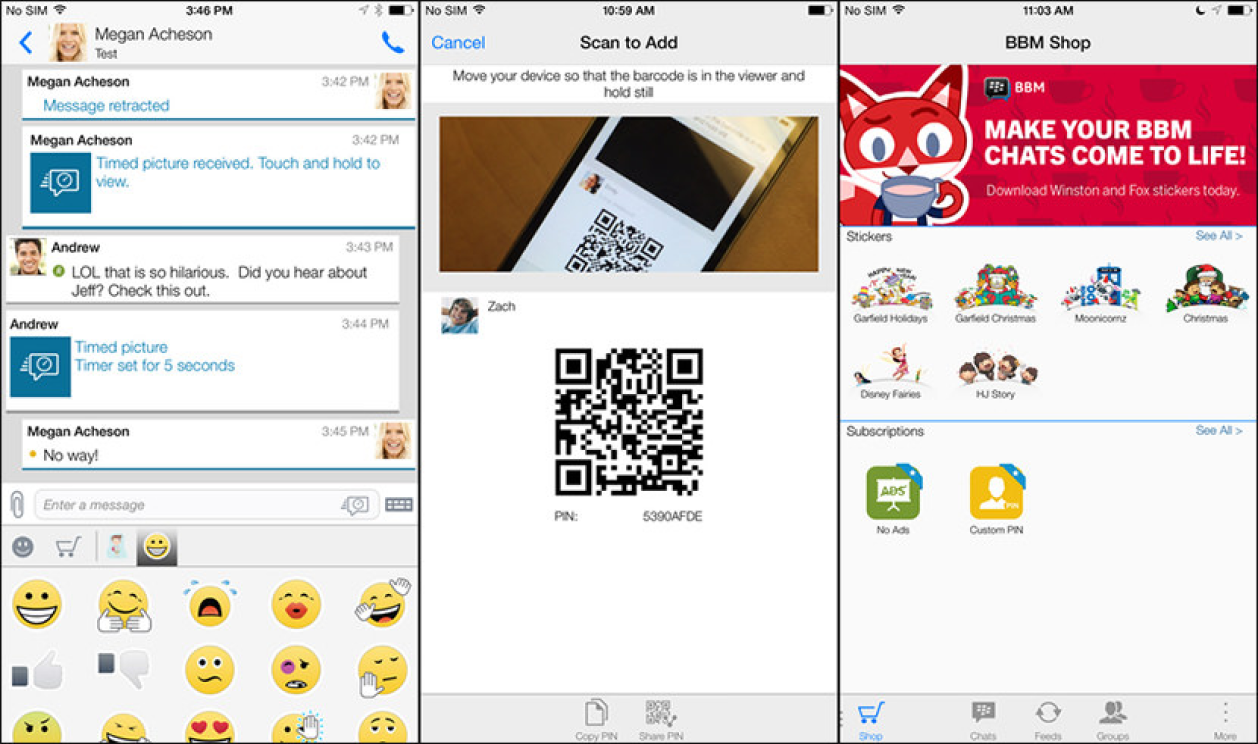
\includegraphics[width=\linewidth]{bilder/research pic/blackberry-messenger-live-free.png}
                                                                                        & \textbf{Blackberry Messenger Live}\newline
    Zuerst haben wir uns umgeschaut und nach Chatfenstern gesucht. Hier haben wir uns die Austauschung von Sprechblasen angeschaut
    und deren Ausrichtung.                                                                                                           \\
    Bildquelle:\cite{blackberry} \newline                                                                                            \\
    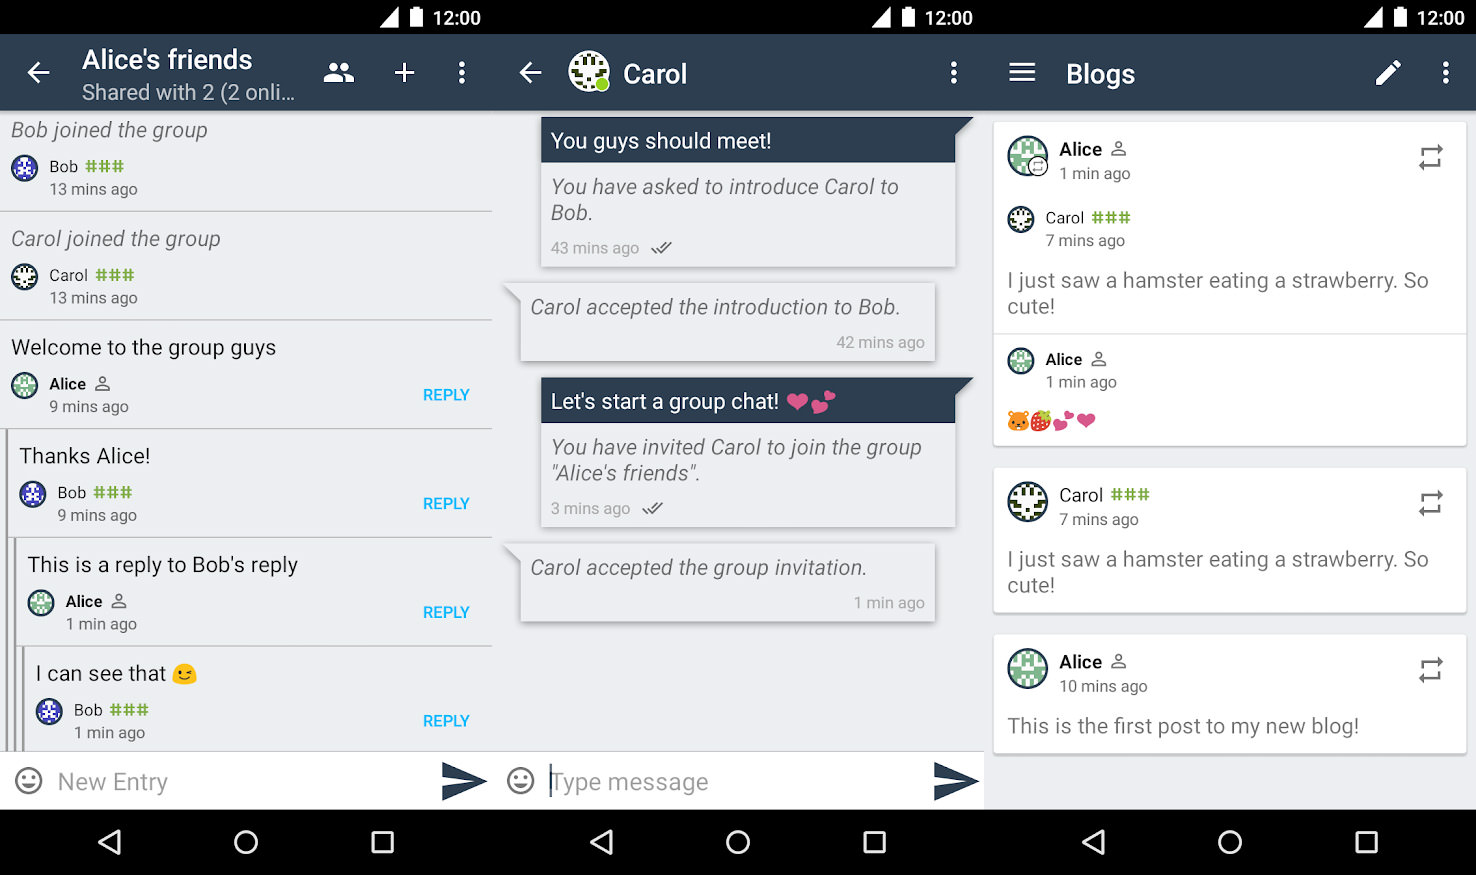
\includegraphics[width=\linewidth]{bilder/research pic/briar.jpg}
                                                                                        & \textbf{Briar} \newline
    In diesem Beispiel haben wir uns wieder das Chatfenster und die verschiedenen Symbole angeschaut.
    Wie das Editierbutton oder das Hinzufügebutton.                                                                                  \\
    Bildquelle:\cite{briar} \newline                                                                                                 \\
    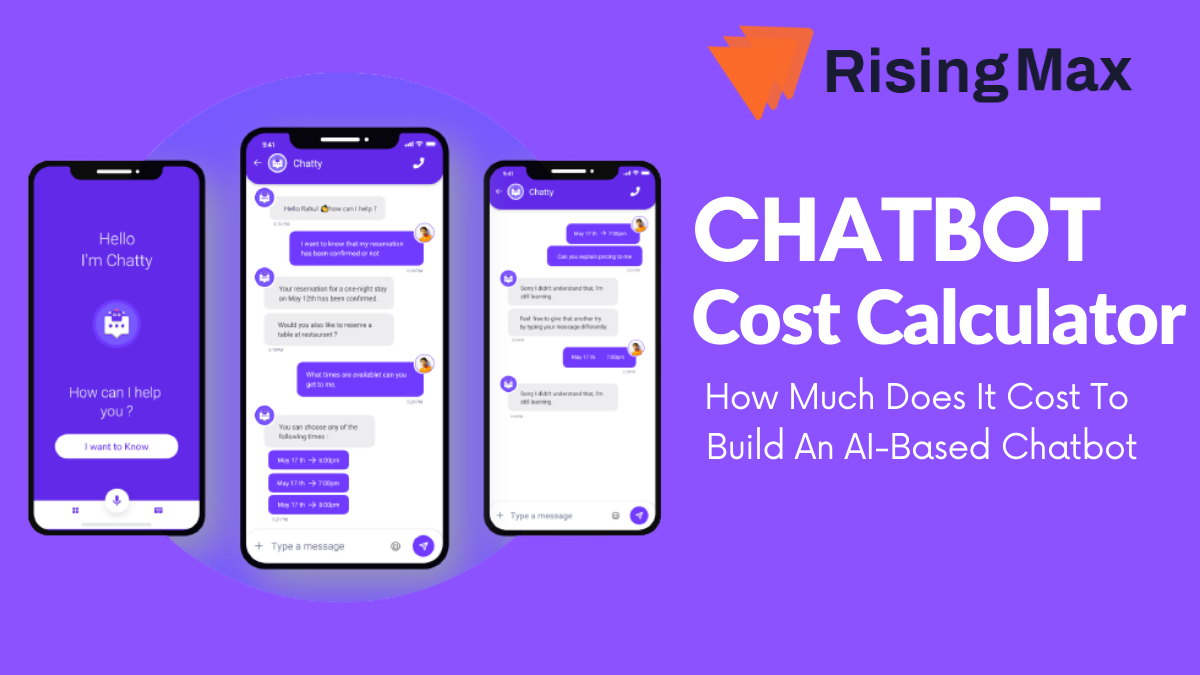
\includegraphics[width=\linewidth]{bilder/research pic/chatbot-cost-calculator.png} & \textbf{CHATBOT Cost Calculator} \newline
    Hier haben wir uns ein ChatBot-Fenster angeschaut und dabei die Icons und die
    verschiedenen Elemente angeschaut, wie den Balken an der Oberseite oder das Sendebutton.                                         \\
    Bildquelle:\cite{chatbotcostcalc} \newline
\end{tabular}

\begin{tabular}{C{6cm}  L{7cm}}
    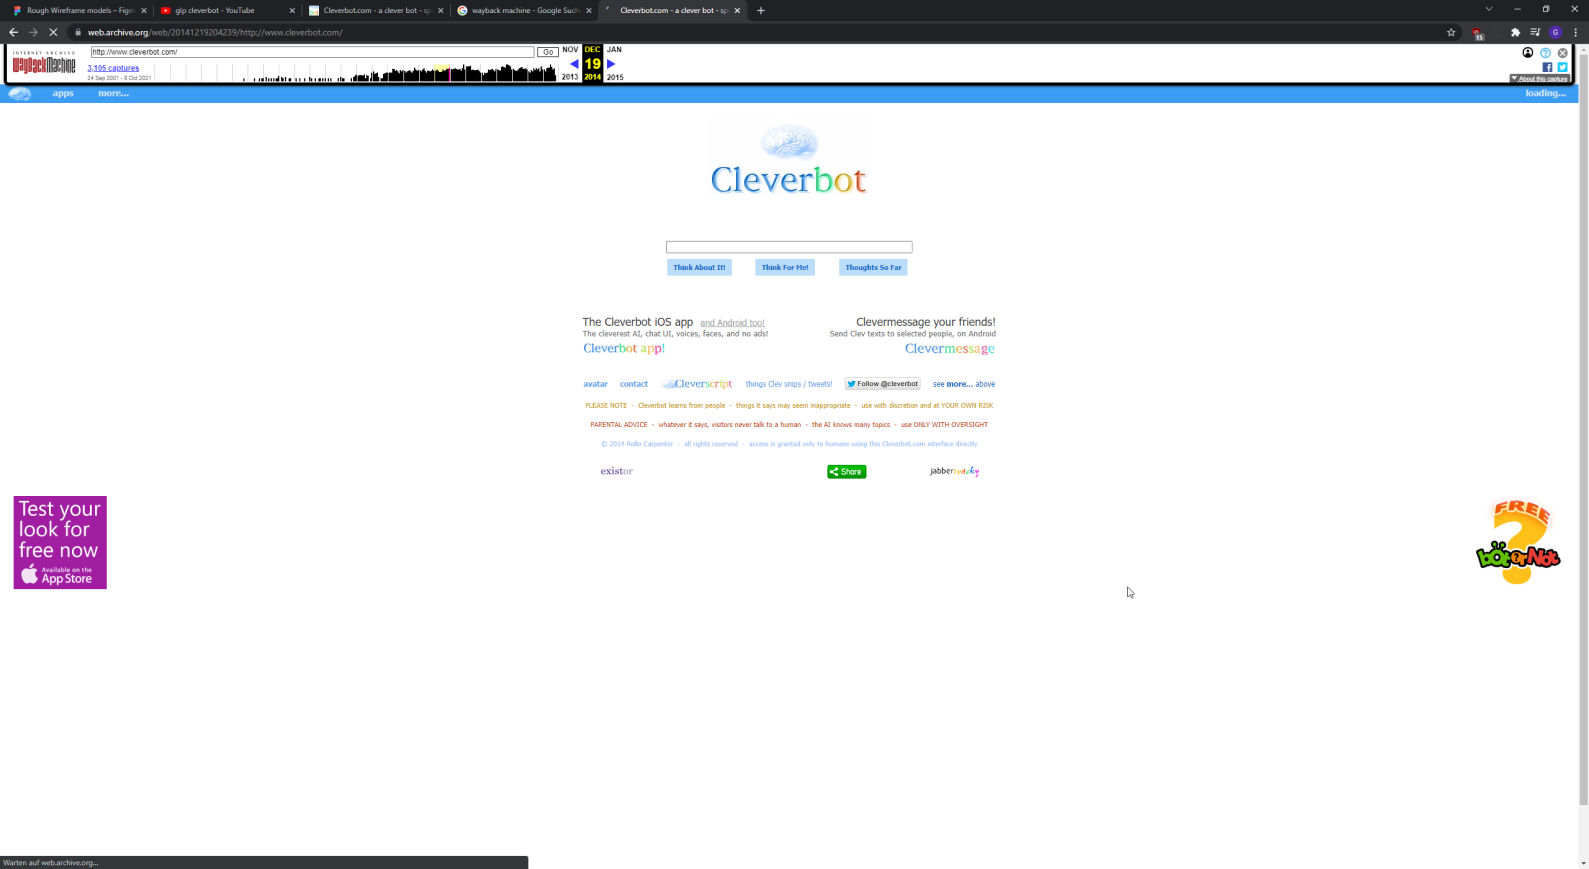
\includegraphics[width=\linewidth]{bilder/research pic/cleverbot.png}                 & \textbf{Cleverbot} \newline
    Diesen Bot haben wir uns genauer angeschaut, weil dieser auch uns bekannt war.                                      \\
    Bildquelle:\cite{cleverbot} \newline
    \\
    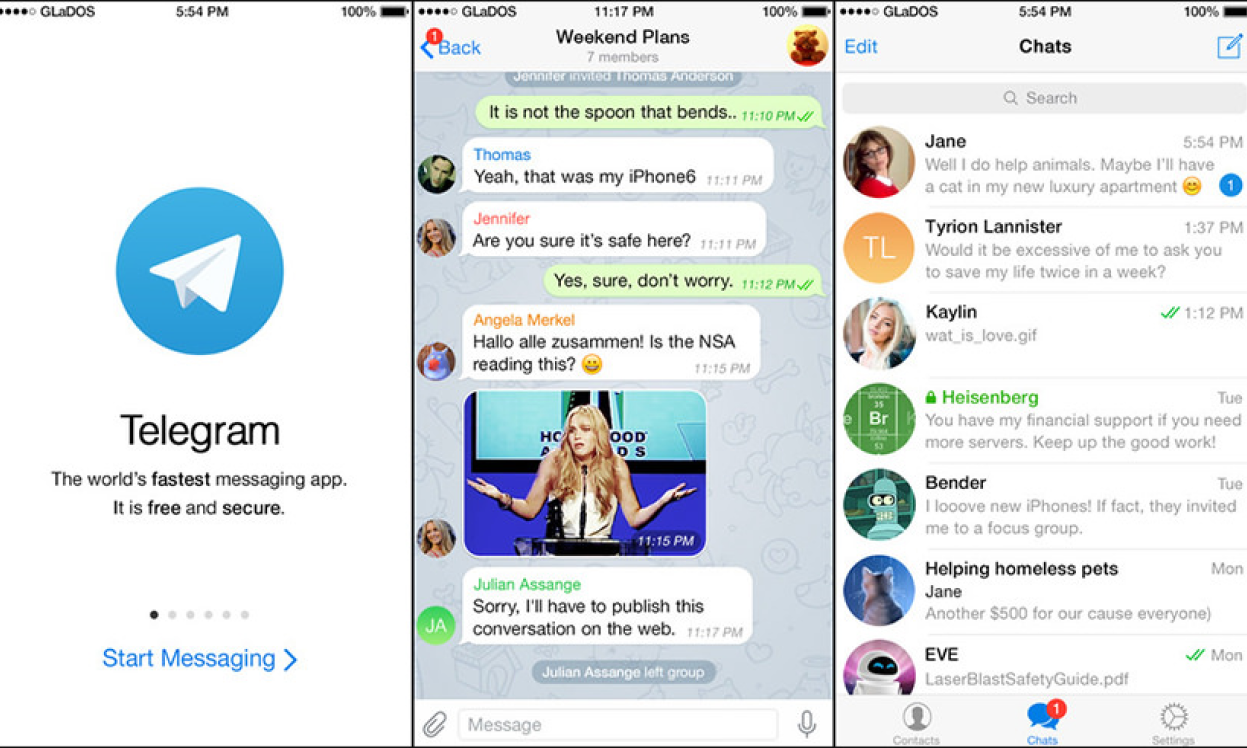
\includegraphics[width=\linewidth]{bilder/research pic/Telegram pic.png}              & \textbf{Telegram} \newline
    Telegram haben wir uns wiederrum das Chatfenster und die Icons angeschaut.                                          \\
    Bildquelle:\cite{telegrambild} \newline
    \\
    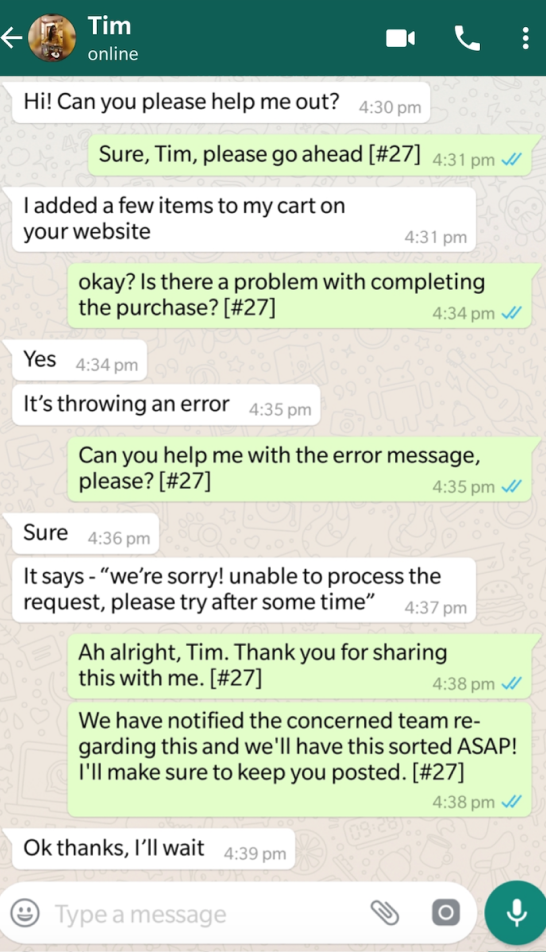
\includegraphics[width=\linewidth, height=12cm]{bilder/research pic/Tim Whatsapp.png} & \textbf{WhatsApp} \newline
    Hier haben wir uns mehr auf die Ausrichtungen des Chatfensters angeschaut und wie die Sprechblasen
    ausgerichtet sind. Fast jeder benutzt WhatsApp deswegen haben wir uns die Struktur angeschaut,
    weil diese viele Benutzer bekannt ist.                                                                              \\
    Bildquelle:\cite{timwhatsApp} \newline
\end{tabular}

\subsection{Erfahrungen zu der Recherche von unseren UI Designs}
In Recherche von den UI Designs haben die einzelnen Komponenten wie der Aufbau eines CHats und 
die Anordnung eine große Rolle gespielt. Die Erfahrungen die man aus den einzelnen Elementen gesammelt hat,
sind:
\\

\noindent Die Chatfenster sind immer gleich aufgebaut. 
Sie haben alle eine große Fläche, wo die Chats angezeigt werden. 
Außerdem haben alle Chat Designs einen Textfield, wo meine seine Fragen und Anliegen schreiben kann. 
Jeder User besitzt ein Profilbild. Sogar der ChatBot besitzt ein Profilbild. 
Das Chatfield vom ChatBot Calculator hat ein gutes Design, wo das Profilbild neben dem Chatfield zu sehen ist.
Demnach ist nachvollziehbar, wer was geschrieben hat. 
Neben dem Textfield, wo man seine Anliegen eingeben kann, steht immer der Sendebutton.
Die Benutzer sind also mehr auf ein UI Design eingestellt, welche Ihnen immer vorgelegt wird.
Darum wird das questMe Chatfenster auch ein UI Design erhalten, welches sich von der 
Basisstruktur der anderen Chats im Alltag nicht unterscheidet.




\subsection{Version 1 von UI-Konzept}

Hier sind die älteren Entwürfe des Designs. Bei diesen Entwürfen haben wir uns nur auf die Struktur
konzentriert und eine grobe Version erstellt. Uns war es hier hauptsächlich wichtig
die Ideen, die wir durch die Recherche aufgenommen haben zu projezieren.
\\

\subsubsection{Version 1 Webchat}
Hier sieht man die älteren UI Designs Versionen, die zum Teil Chantfenster gehören.

\begin{figure}[H]
    \centering
    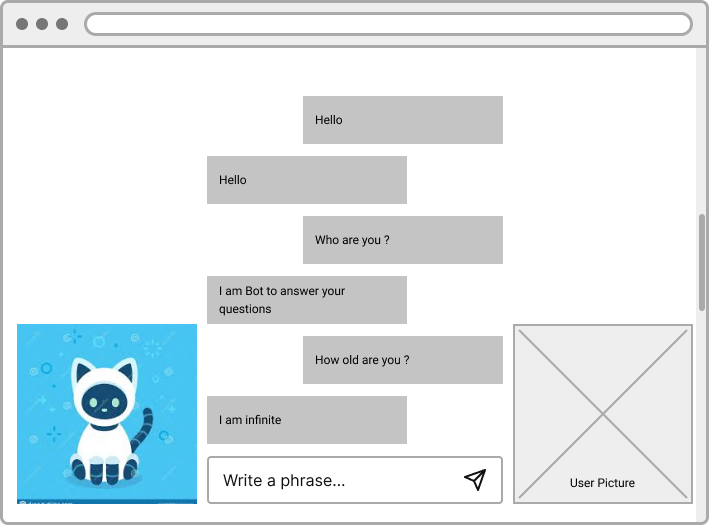
\includegraphics[width=0.8\textwidth]{bilder/old vers. UI Design/WebChat.png}
    \caption{old version UI Design WebChat}
    \label{fig:old version UI Design WebChat}
    \end{figure}
\noindent \textbf{Webchat} \newline
In der alten Version unseres Webchat designs haben wir gedacht, auch für den
Nutzer ein Profilbild hinzu zufügen. Diese Idee aber schien zu aufwendig zu sein und wir versuchen
zuerst ein Minimal Viable Product zu erschaffen.                                                     

\newpage

\subsubsection{Version 1 Admin Interface Allgemein}
Hier sieht man die älteren UI Designs Versionen, die zum Teil Admin-Interface Allgemein gehören.

\begin{figure}[H]
    \centering
    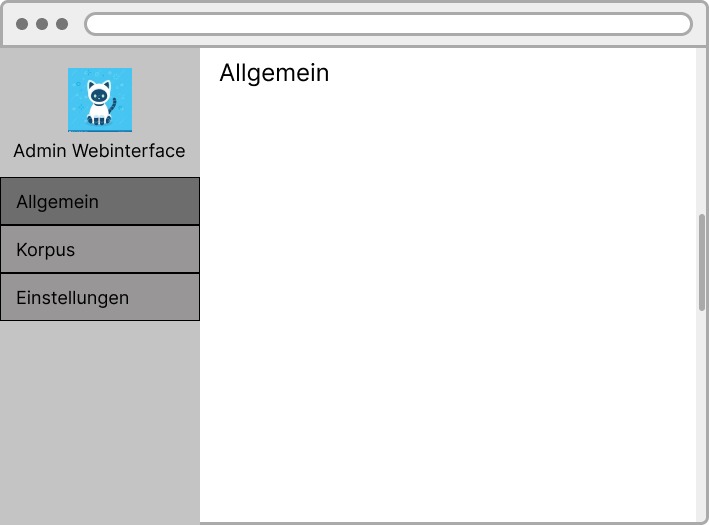
\includegraphics[width=0.8\textwidth]{bilder/old vers. UI Design/Admin Interface Allgemein.png}
    \caption{old version UI Design Admin Interface Allgemein}
    \label{fig:old version UI Design Admin Interface Allgemein}
    \end{figure}
\noindent \textbf{Admin Interface: Allgemein} \newline
Im Admin Interface kann man auf der linken Seite das Menü sehen. Was aber hier fehlt ist der Logout Button.
Wir hatten auch keine richtigen Vorstellungen, was wir einführen möchten.

\newpage

\subsubsection{Version 1 Admin Interface Korpus}
Hier sieht man die älteren UI Designs Versionen, die zum Teil Admin-Interface Korpus gehören.

\begin{figure}[H]
    \centering
    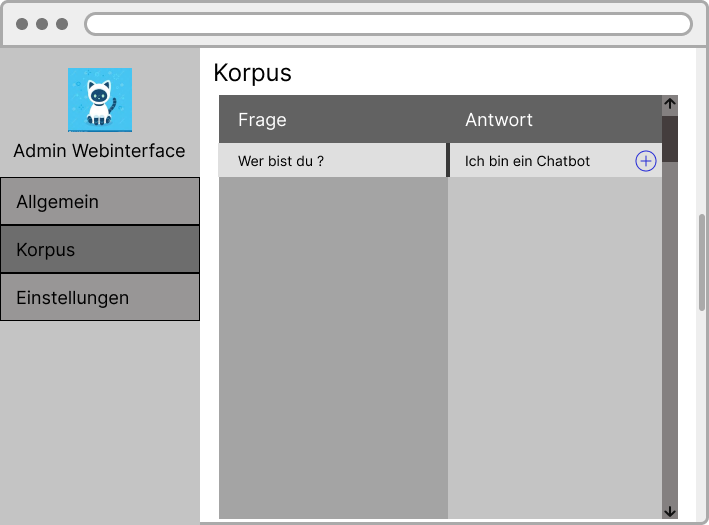
\includegraphics[width=0.8\textwidth]{bilder/old vers. UI Design/Admin Interface (1).png}
    \caption{old version UI Design Admin Interface Korpus 00}
    \label{fig:old version UI Design Admin Interface Korpus 00}
    \end{figure}
\noindent \textbf{Admin Interface: Korpus 00} \newline
Im Korpus wollten wir schon von Anfang an das Hinzufügen darstellen, wussten aber nicht
wie und haben herumprobiert.

\begin{figure}[H]
    \centering
    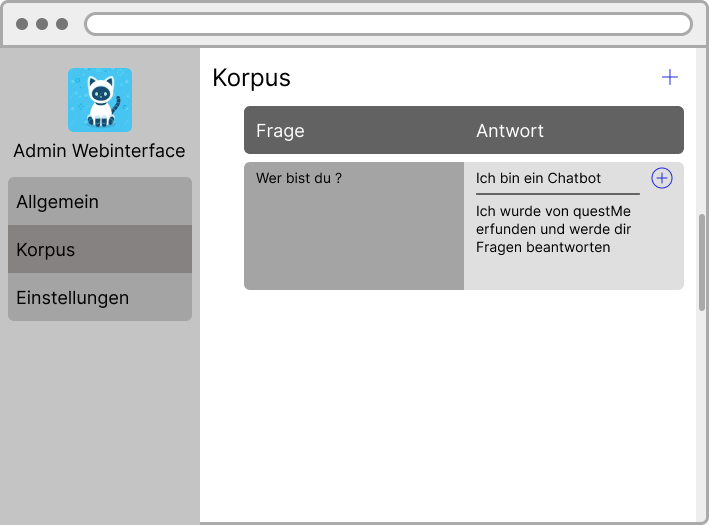
\includegraphics[width=0.8\textwidth]{bilder/old vers. UI Design/Admin Interface I.png}
    \caption{old version UI Design Admin Interface Korpus 01}
    \label{fig:old version UI Design Admin Interface Korpus 01}
    \end{figure}
\noindent \textbf{Admin Interface: Korpus 01} \newline
In diesem Beispiel sieht man ein Basisbeispiel mit einer Frage die im Alltag gestellt wird und die dazugehörenden Antworten. Wie wir diese aber
editieren haben wir hier noch nicht gezeigt.

\begin{figure}[H]
    \centering
    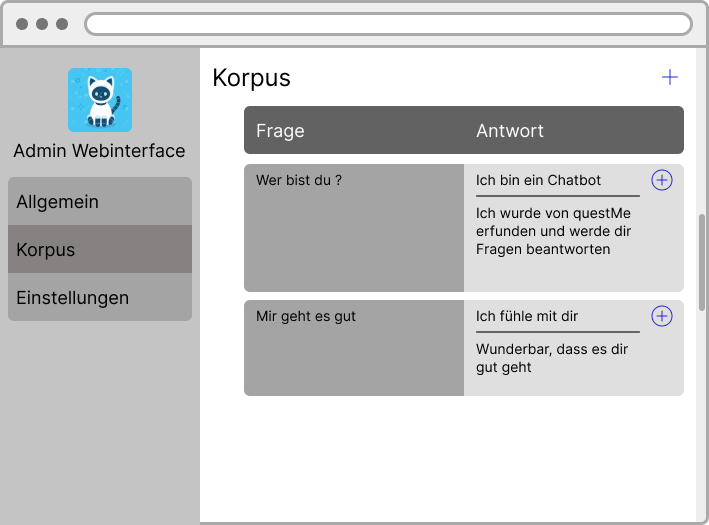
\includegraphics[width=0.8\textwidth]{bilder/old vers. UI Design/Admin Interface II.png}
    \caption{old version UI Design Admin Interface Korpus 02}
    \label{fig:old version UI Design Admin Interface Korpus 02}
    \end{figure}
\noindent \textbf{Admin Interface: Korpus 02} \newline
Im nächsten Beispiel sieht man eine weitere Frage und die dazugehörenden zwei Antworten. Es ist immer noch nicht
bekannt, wie man Antworten und Fragen editiert oder Fragen und Antworten von verschiedenen Domänen bearbeitet.

\newpage

\subsubsection{Version 1 Admin Interface Login}
Hier sieht man die älteren UI Designs Versionen, die zum Teil Admin-Interface Login gehören.

\begin{figure}[H]
    \centering
    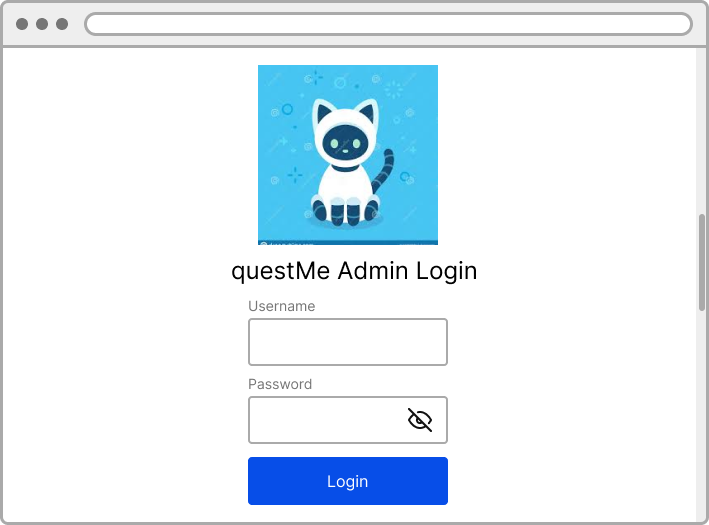
\includegraphics[width=0.8\textwidth]{bilder/old vers. UI Design/Admin Interface.png}
    \caption{old version UI Design Admin Interface Login}
    \label{fig:old version UI Design Admin Interface Login}
    \end{figure}
\noindent \textbf{Admin Interface: Admin Login} \newline
Hier haben wir nur einen klassischen Login Eingabefeld dargestellt, weil wir uns nicht klar waren, wie es mit der Athentifizierung und dem Admin
Login funktioniert.


\newpage

\subsection{Version 2 von UI-Konzept}
Hier sieht man die neuen Entwürfe des UI Designs. In der neuen Version werden auch die 
"mobilen Versionen" entworfen. Weil der Plan ist zuerst eine mobile first Anwendung herzustellen.

\subsubsection{Version 2 Webchat}
Hier werden die neueren Versionen des UI Designs für den Webchat vorgestellt.
\begin{figure}[H]
    \centering
    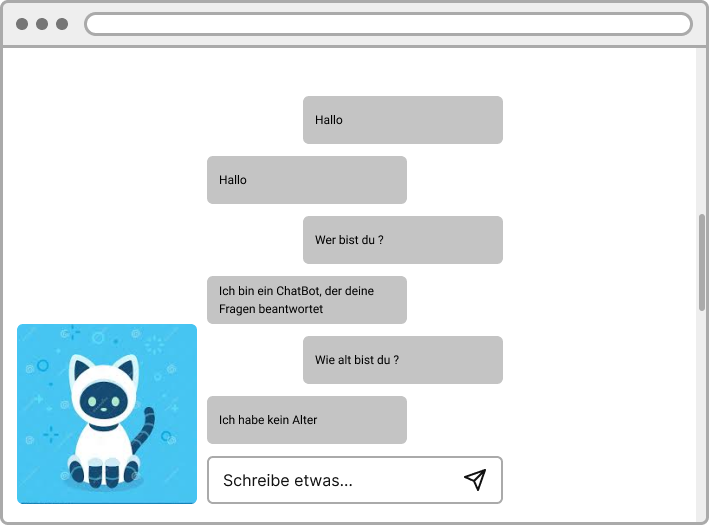
\includegraphics[width=0.8\textwidth]{bilder/new vers. UI Design/WebChat/WebChat.png}
    \caption{new version UI Design Webchat}
    \label{fig:new version UI Design Webchat}
    \end{figure}
\noindent \textbf{Webchat} \newline
Hier haben wir einen Beispielchat mit dem Bot dargestellt. In diesem Beispiel haben wir ein
Basisgespräch geführt.

\begin{figure}[H]
    \centering
    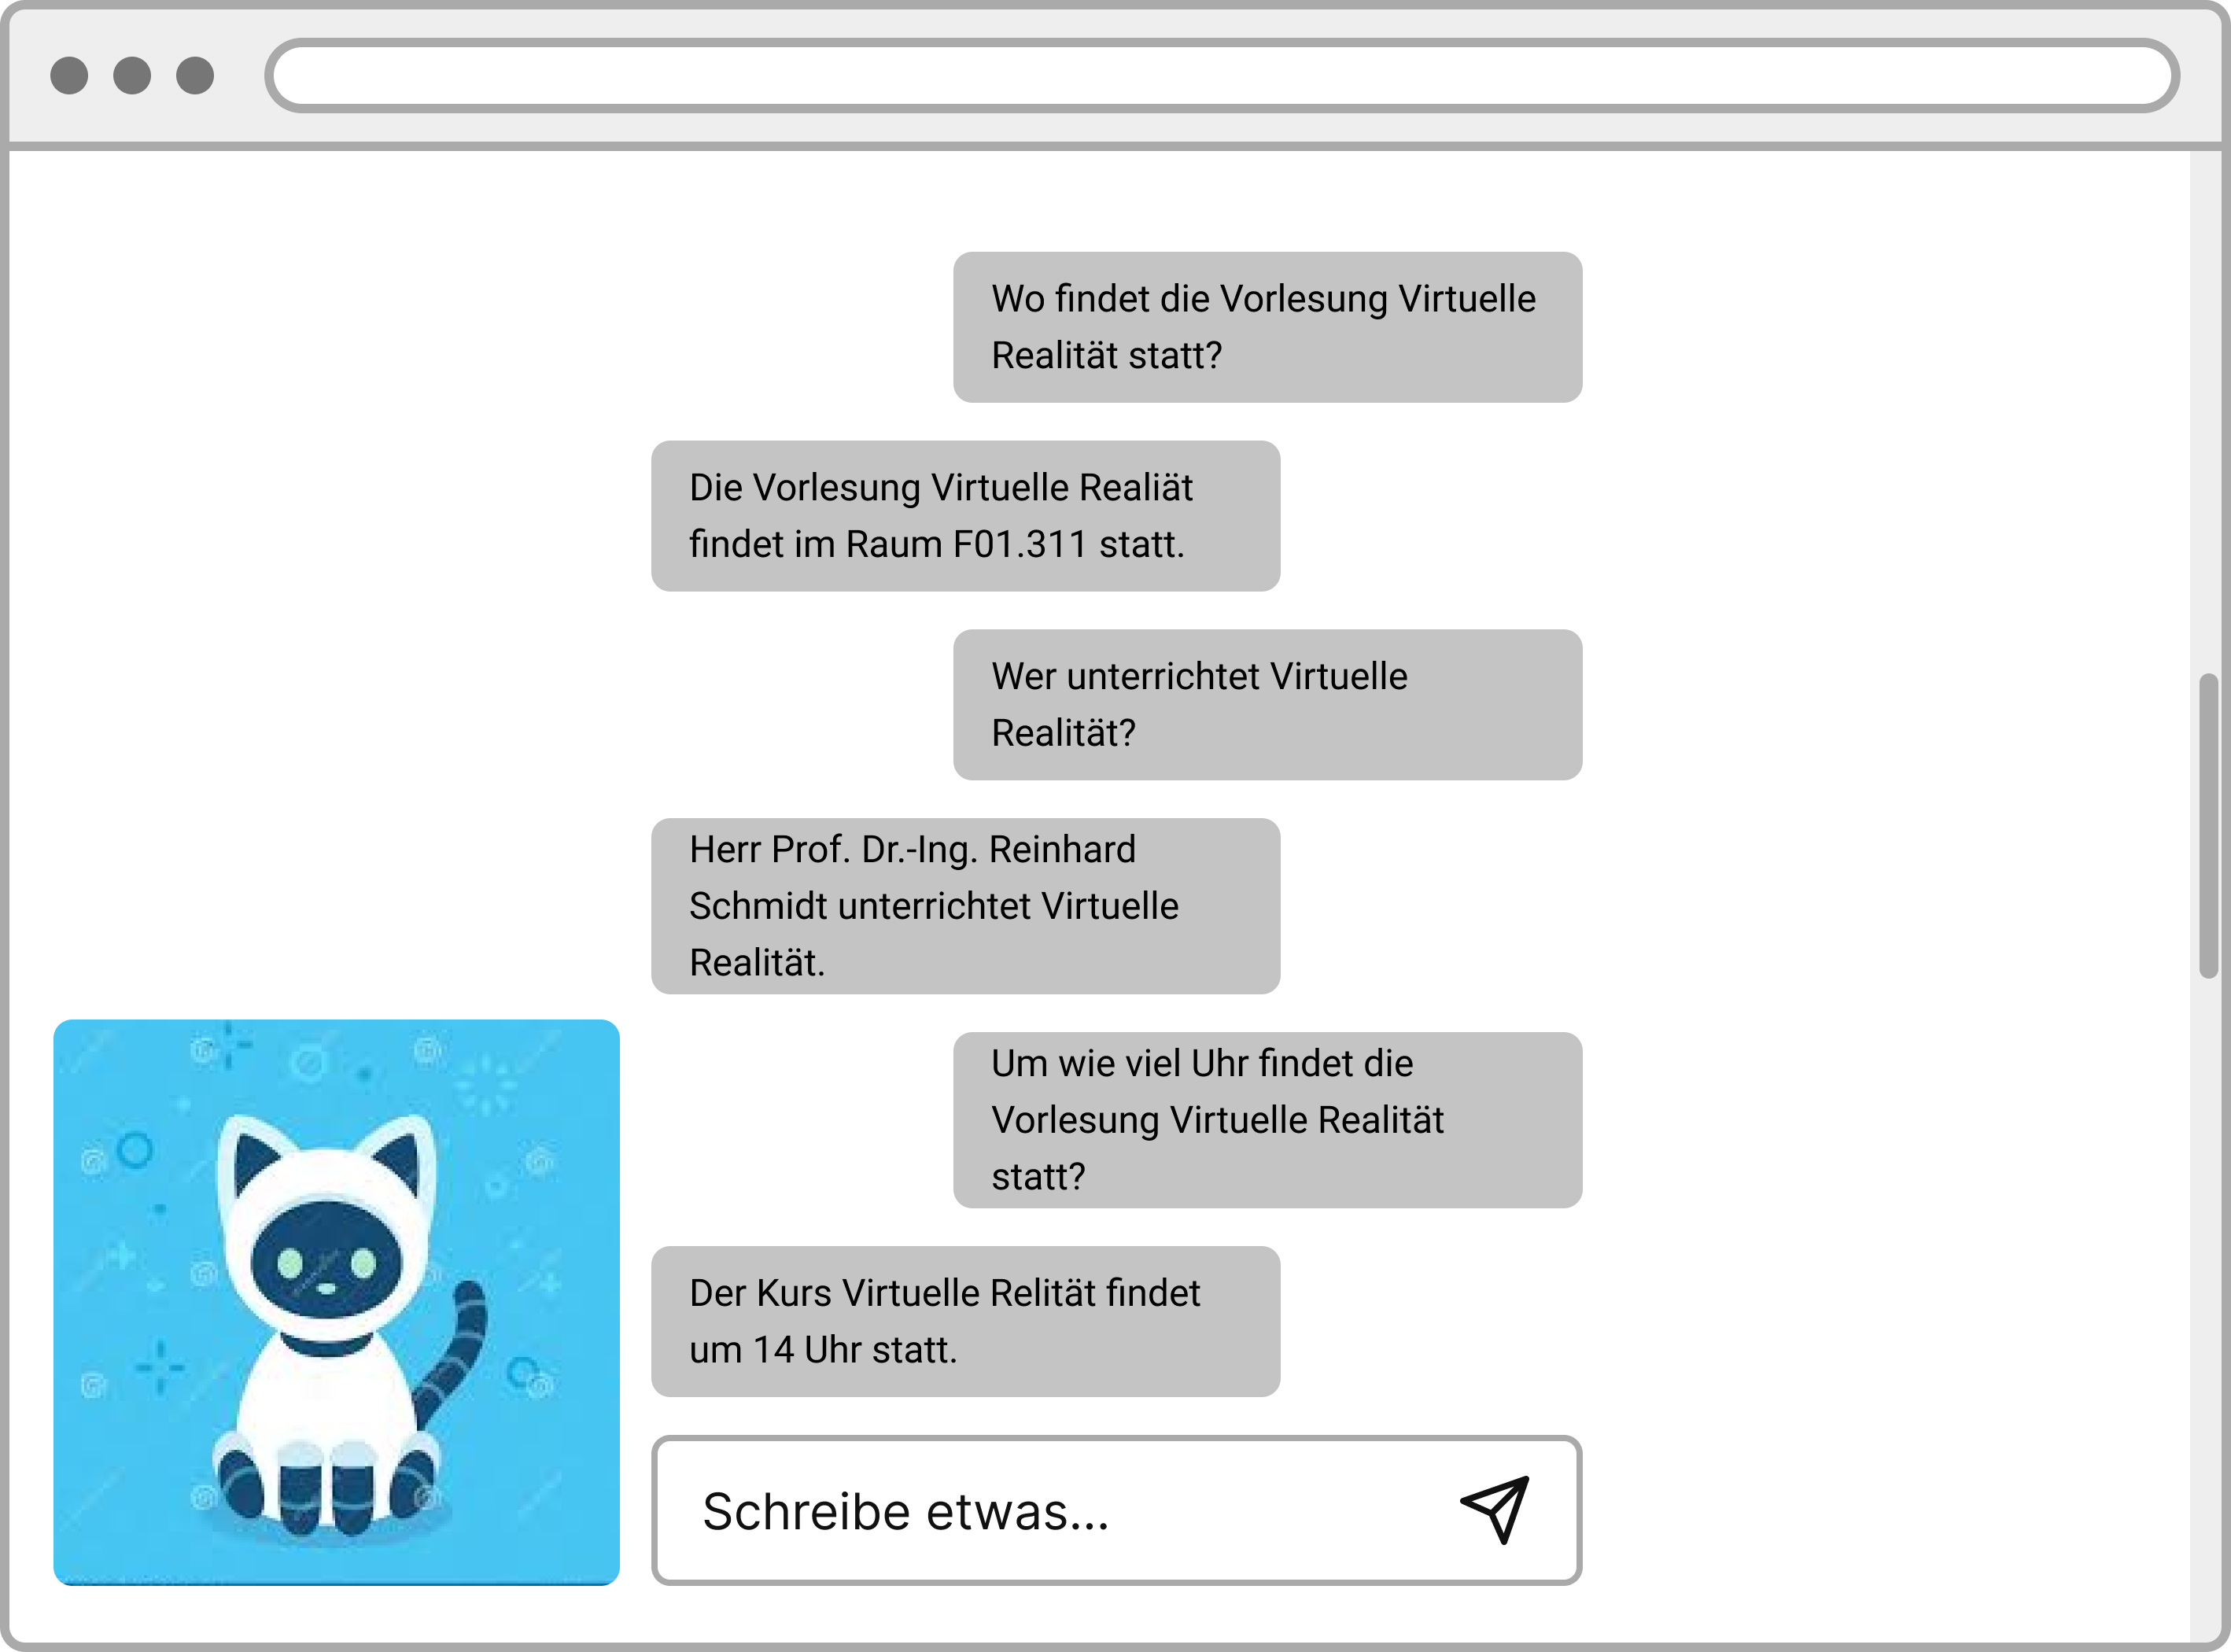
\includegraphics[width=0.8\textwidth]{bilder/new vers. UI Design/WebChat/WebChat Hochschule.png}
    \caption{new version UI Design Webchat Hochschuldomäne}
    \label{fig:new version UI Design Webchat Hochschuldomäne}
    \end{figure}
\noindent \textbf{Webchat mit der Hochschuldomäne} \newline
Diesmal haben wir konkrete Hochschulfragen gestellt und die Hochschuldomäne dargestellt.

\begin{figure}[H]
    \centering
    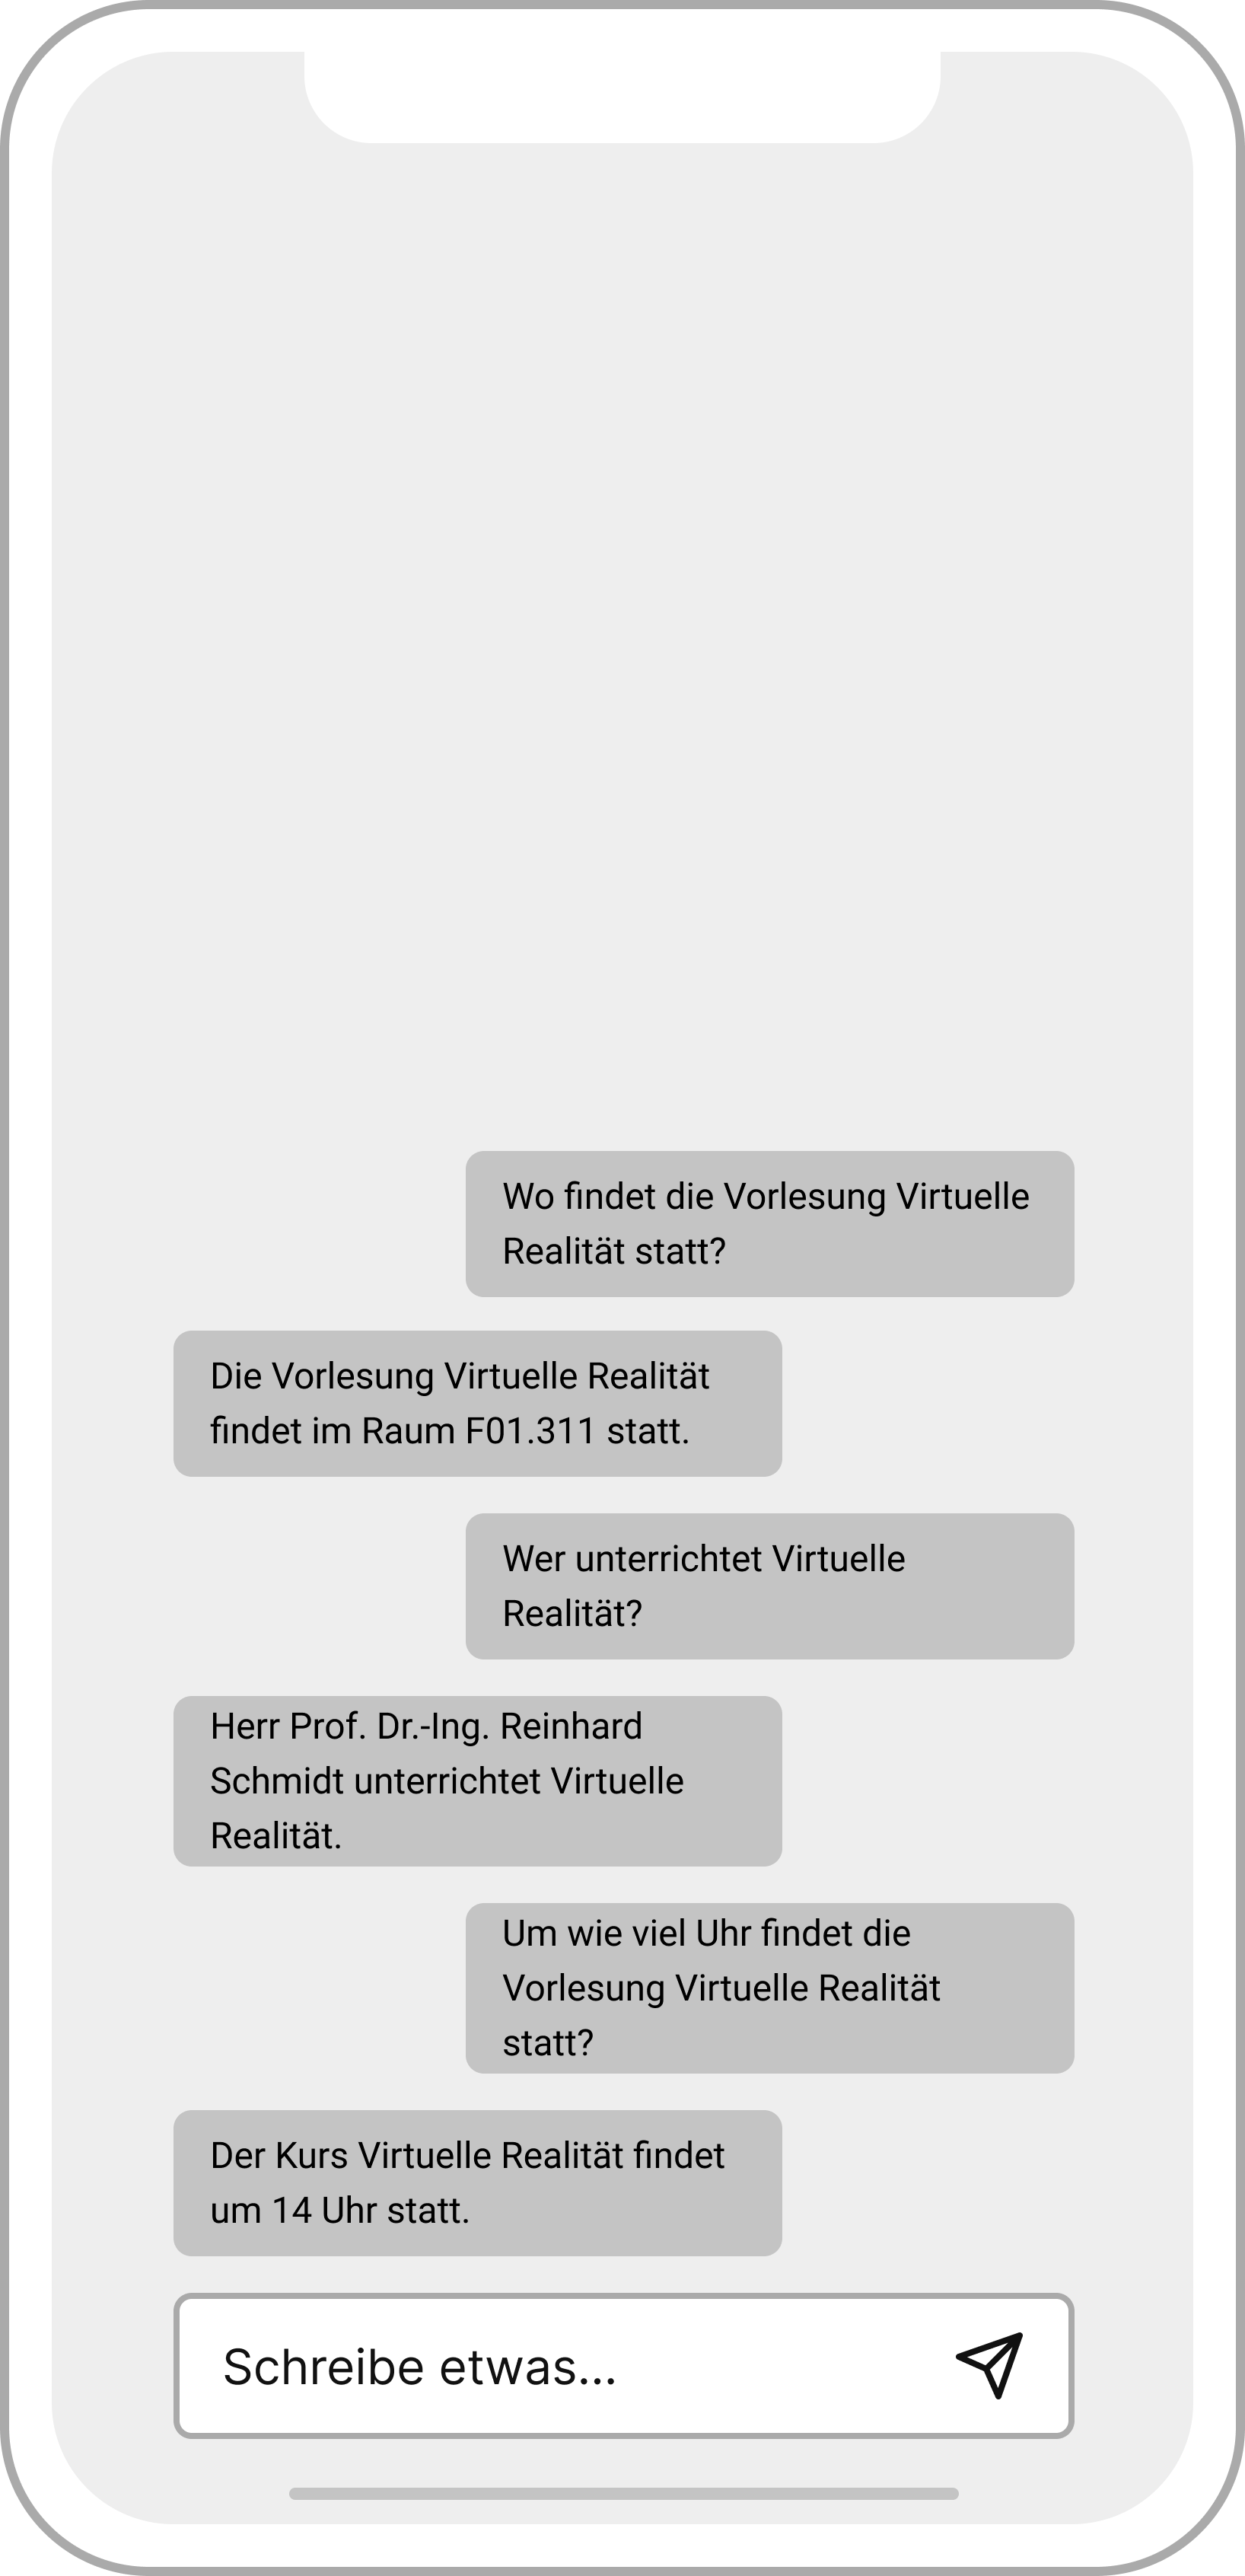
\includegraphics[width=0.5\textwidth]{bilder/new vers. UI Design/WebChat/mobile Version Webchat.png}
    \caption{new version UI Design Webchat mobile version}
    \label{fig:new version UI Design Webchat mobile version}
    \end{figure}
\noindent \textbf{Webchat als mobile Version} \newline
Dies ist die mobile Version des Webchats. Wir haben die Darstellung so einfach wie möglich dargestellt.
Hier haben wir auch die Hochschulbezogenen Fragen gestellt.

\newpage

\subsubsection{Version 2 Admin Interface Allgemein}
Hier werden die neueren Versionen des UI Designs für das Admin-Interface Allgemein vorgestellt

\begin{figure}[H]
    \centering
    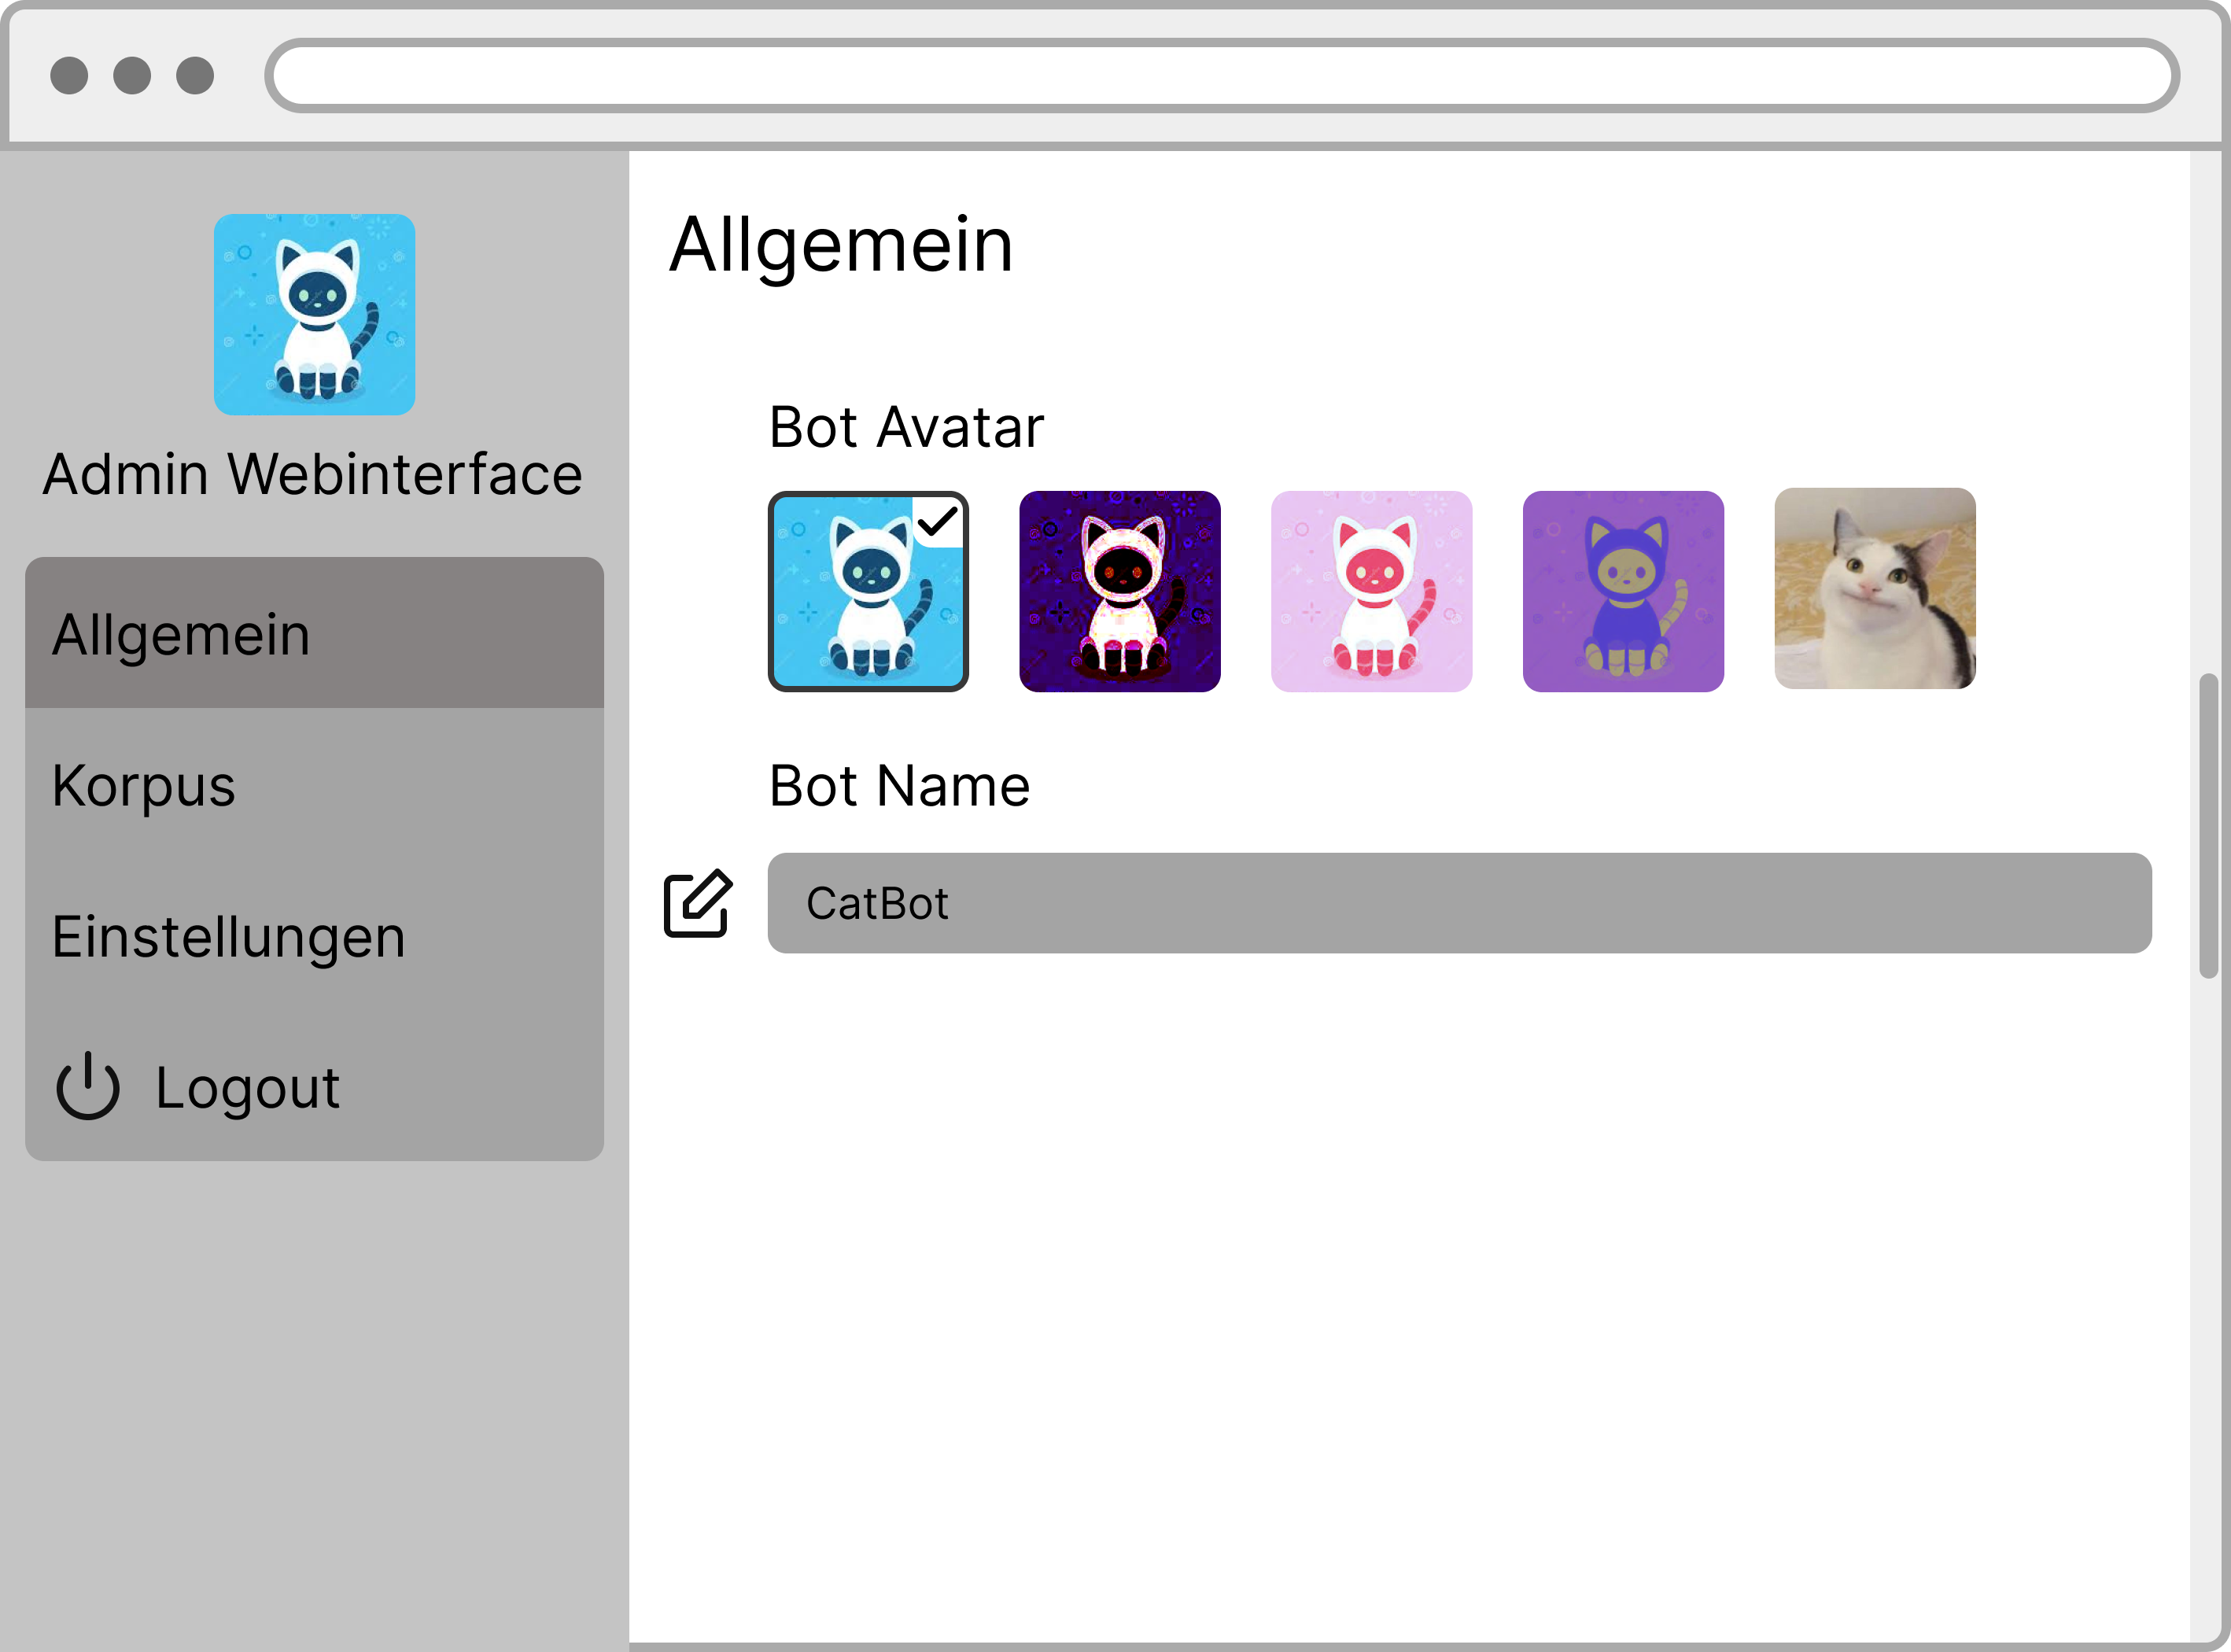
\includegraphics[width=0.8\textwidth]{bilder/new vers. UI Design/Allgemein/Allgemein.png}
    \caption{new version UI Design Admin-Interface Allgemein}
    \label{fig:new version UI Design Admin-Interface Allgemein}
    \end{figure}
\noindent \textbf{Admin Webinterface: Allgemein} \newline
Auf der linken Seite sieht man die Kategorien, die der Admin bearbeiten kann. Im Allgemeinen kann
der Admin den Bot Avatar wechseln, diese wird dann mit einem Haken gekennzeichnet. Außerdem kann
der Admin den Bot Namen ändern, indem er den Editierbutton drückt.

\begin{figure}[H]
    \centering
    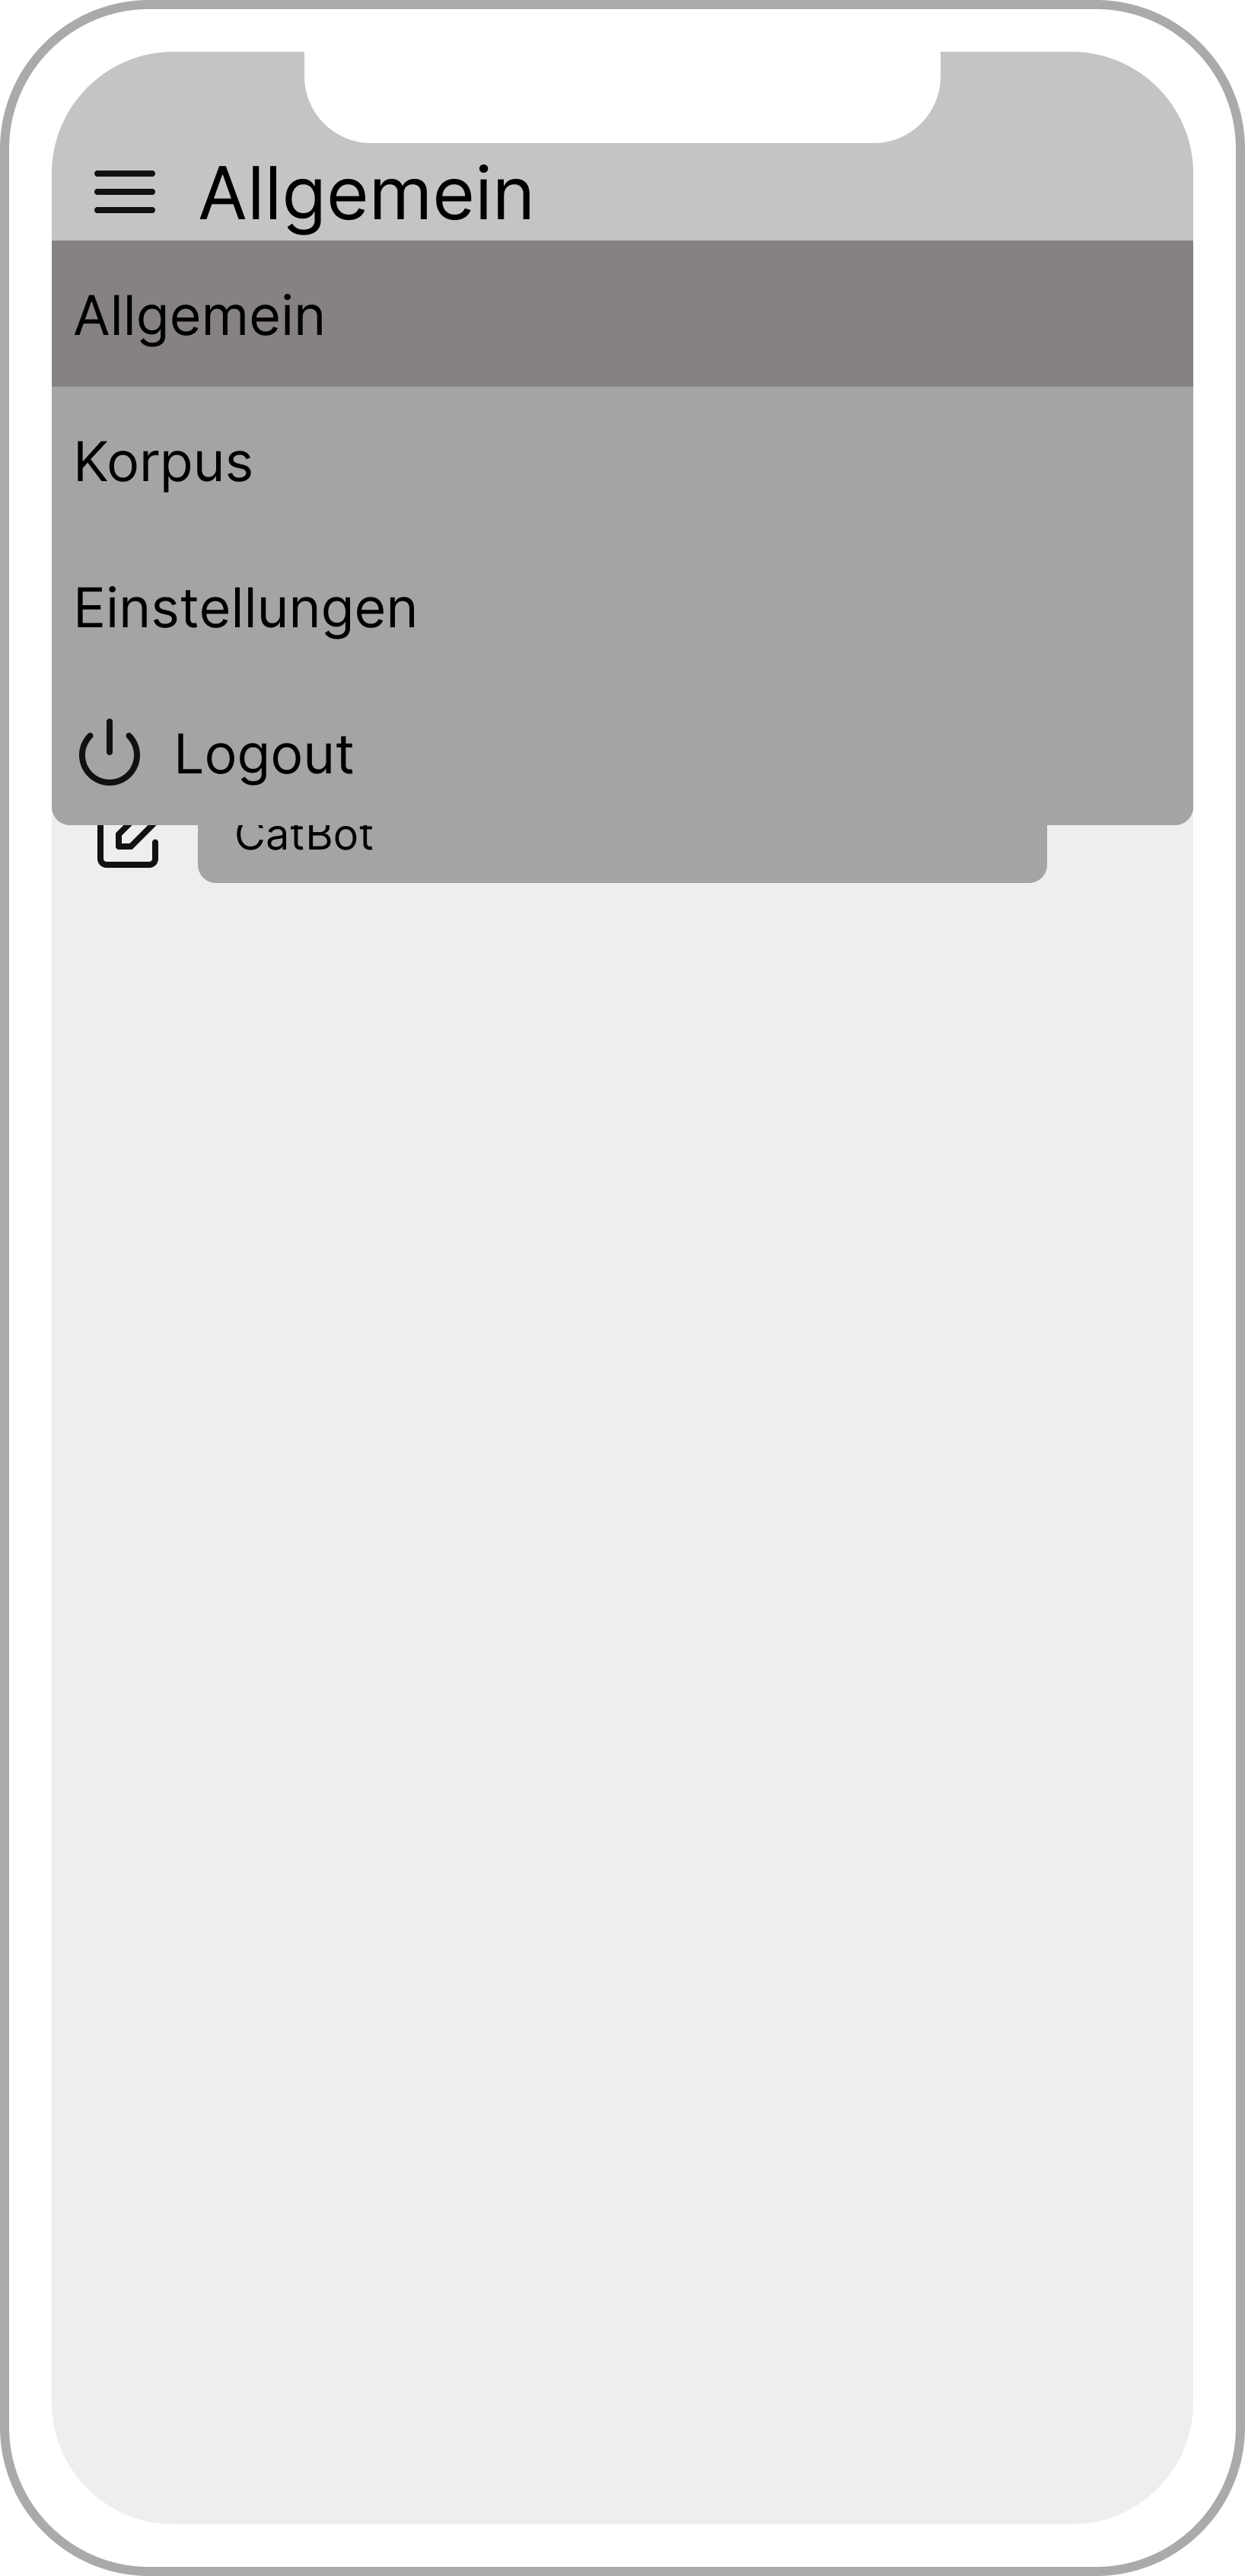
\includegraphics[width=0.5\textwidth]{bilder/new vers. UI Design/Allgemein/iPhone X Allgemein dropdown.png}
    \caption{new version UI Design Admin-Interface Allgemein dropdown menu}
    \label{fig:new version UI Design Admin-Interface Allgemein dropdown menu}
\end{figure}
\noindent \textbf{Admin Webinterface mobil: Allgemein dropdown Menü} \newline
In der mobilen Version haben wir die Kategorien, die der Admin bearbeiten kann im dropdown Menü dargestellt.

\begin{figure}[H]
    \centering
    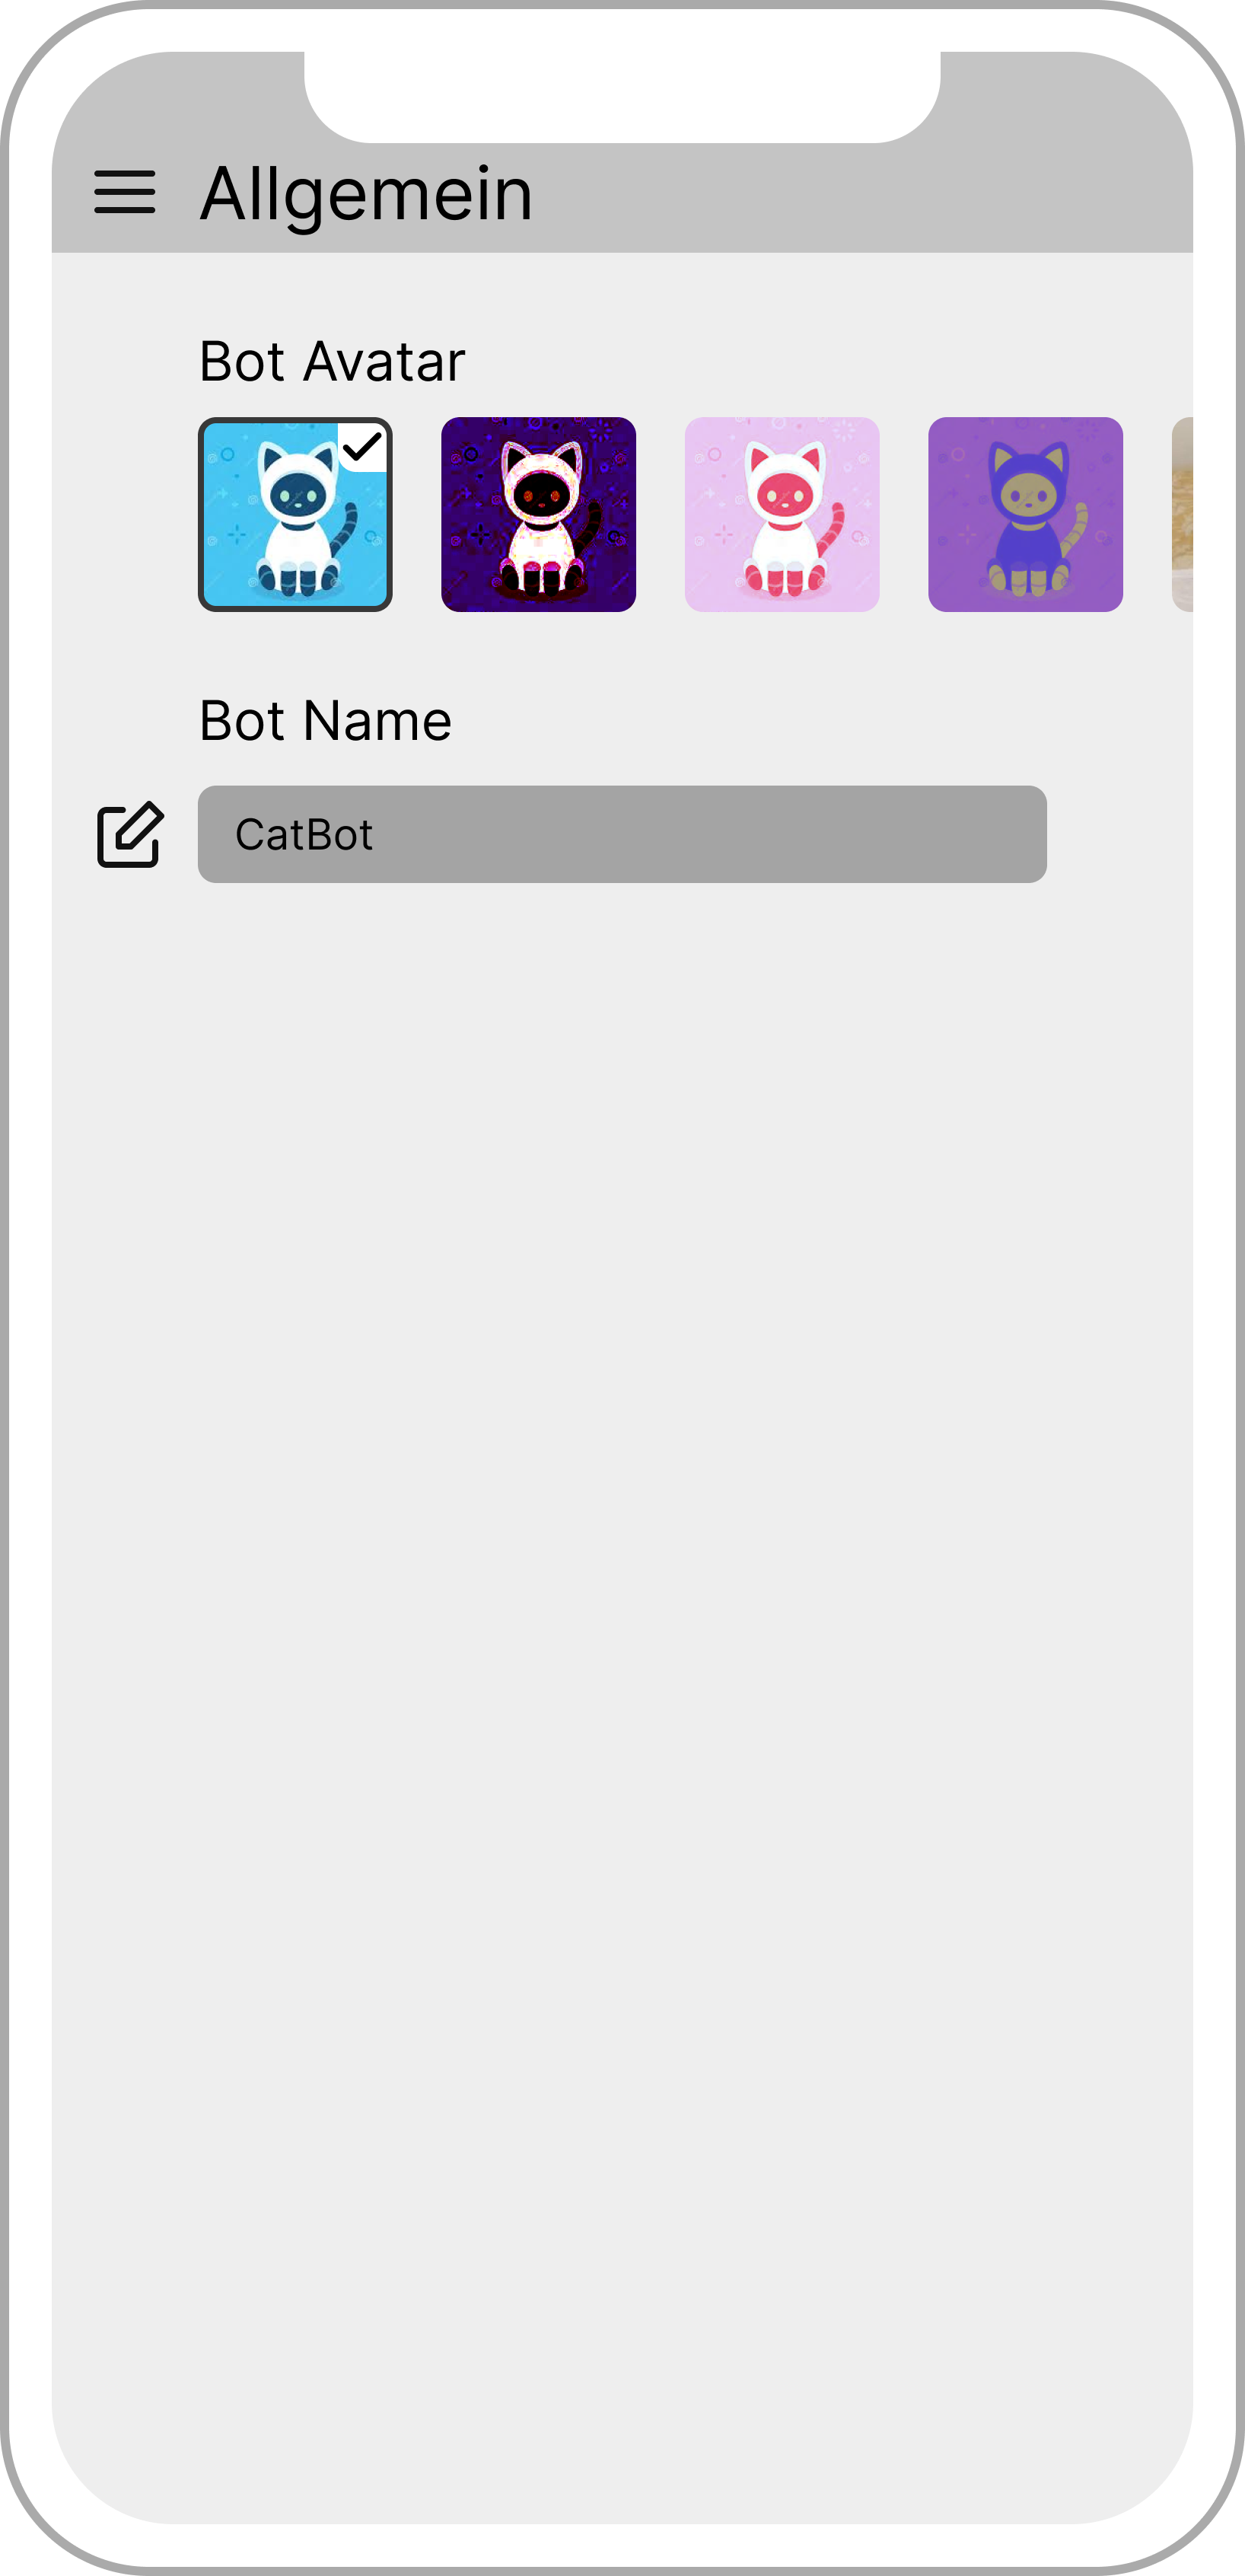
\includegraphics[width=0.5\textwidth]{bilder/new vers. UI Design/Allgemein/iPhone X Allgemein III.png}
    \caption{new version UI Design Admin-Interface Allgemein mobile version}
    \label{fig:new version UI Design Admin-Interface Allgemein mobile version}
\end{figure}
\noindent \textbf{Admin Webinterface mobil: Allgemein} \newline
Die mobile Variante funktioniert genauso wie die Webvariante. Man kann den Bot Avatar wechseln und den
ChatBot Namen frei bestimmen.

\newpage

\subsubsection{Version 2 Admin Interface Korpus}
Hier werden die neueren Versionen des UI Designs für das Admin-Interface Korpus vorgestellt

\begin{figure}[H]
    \centering
    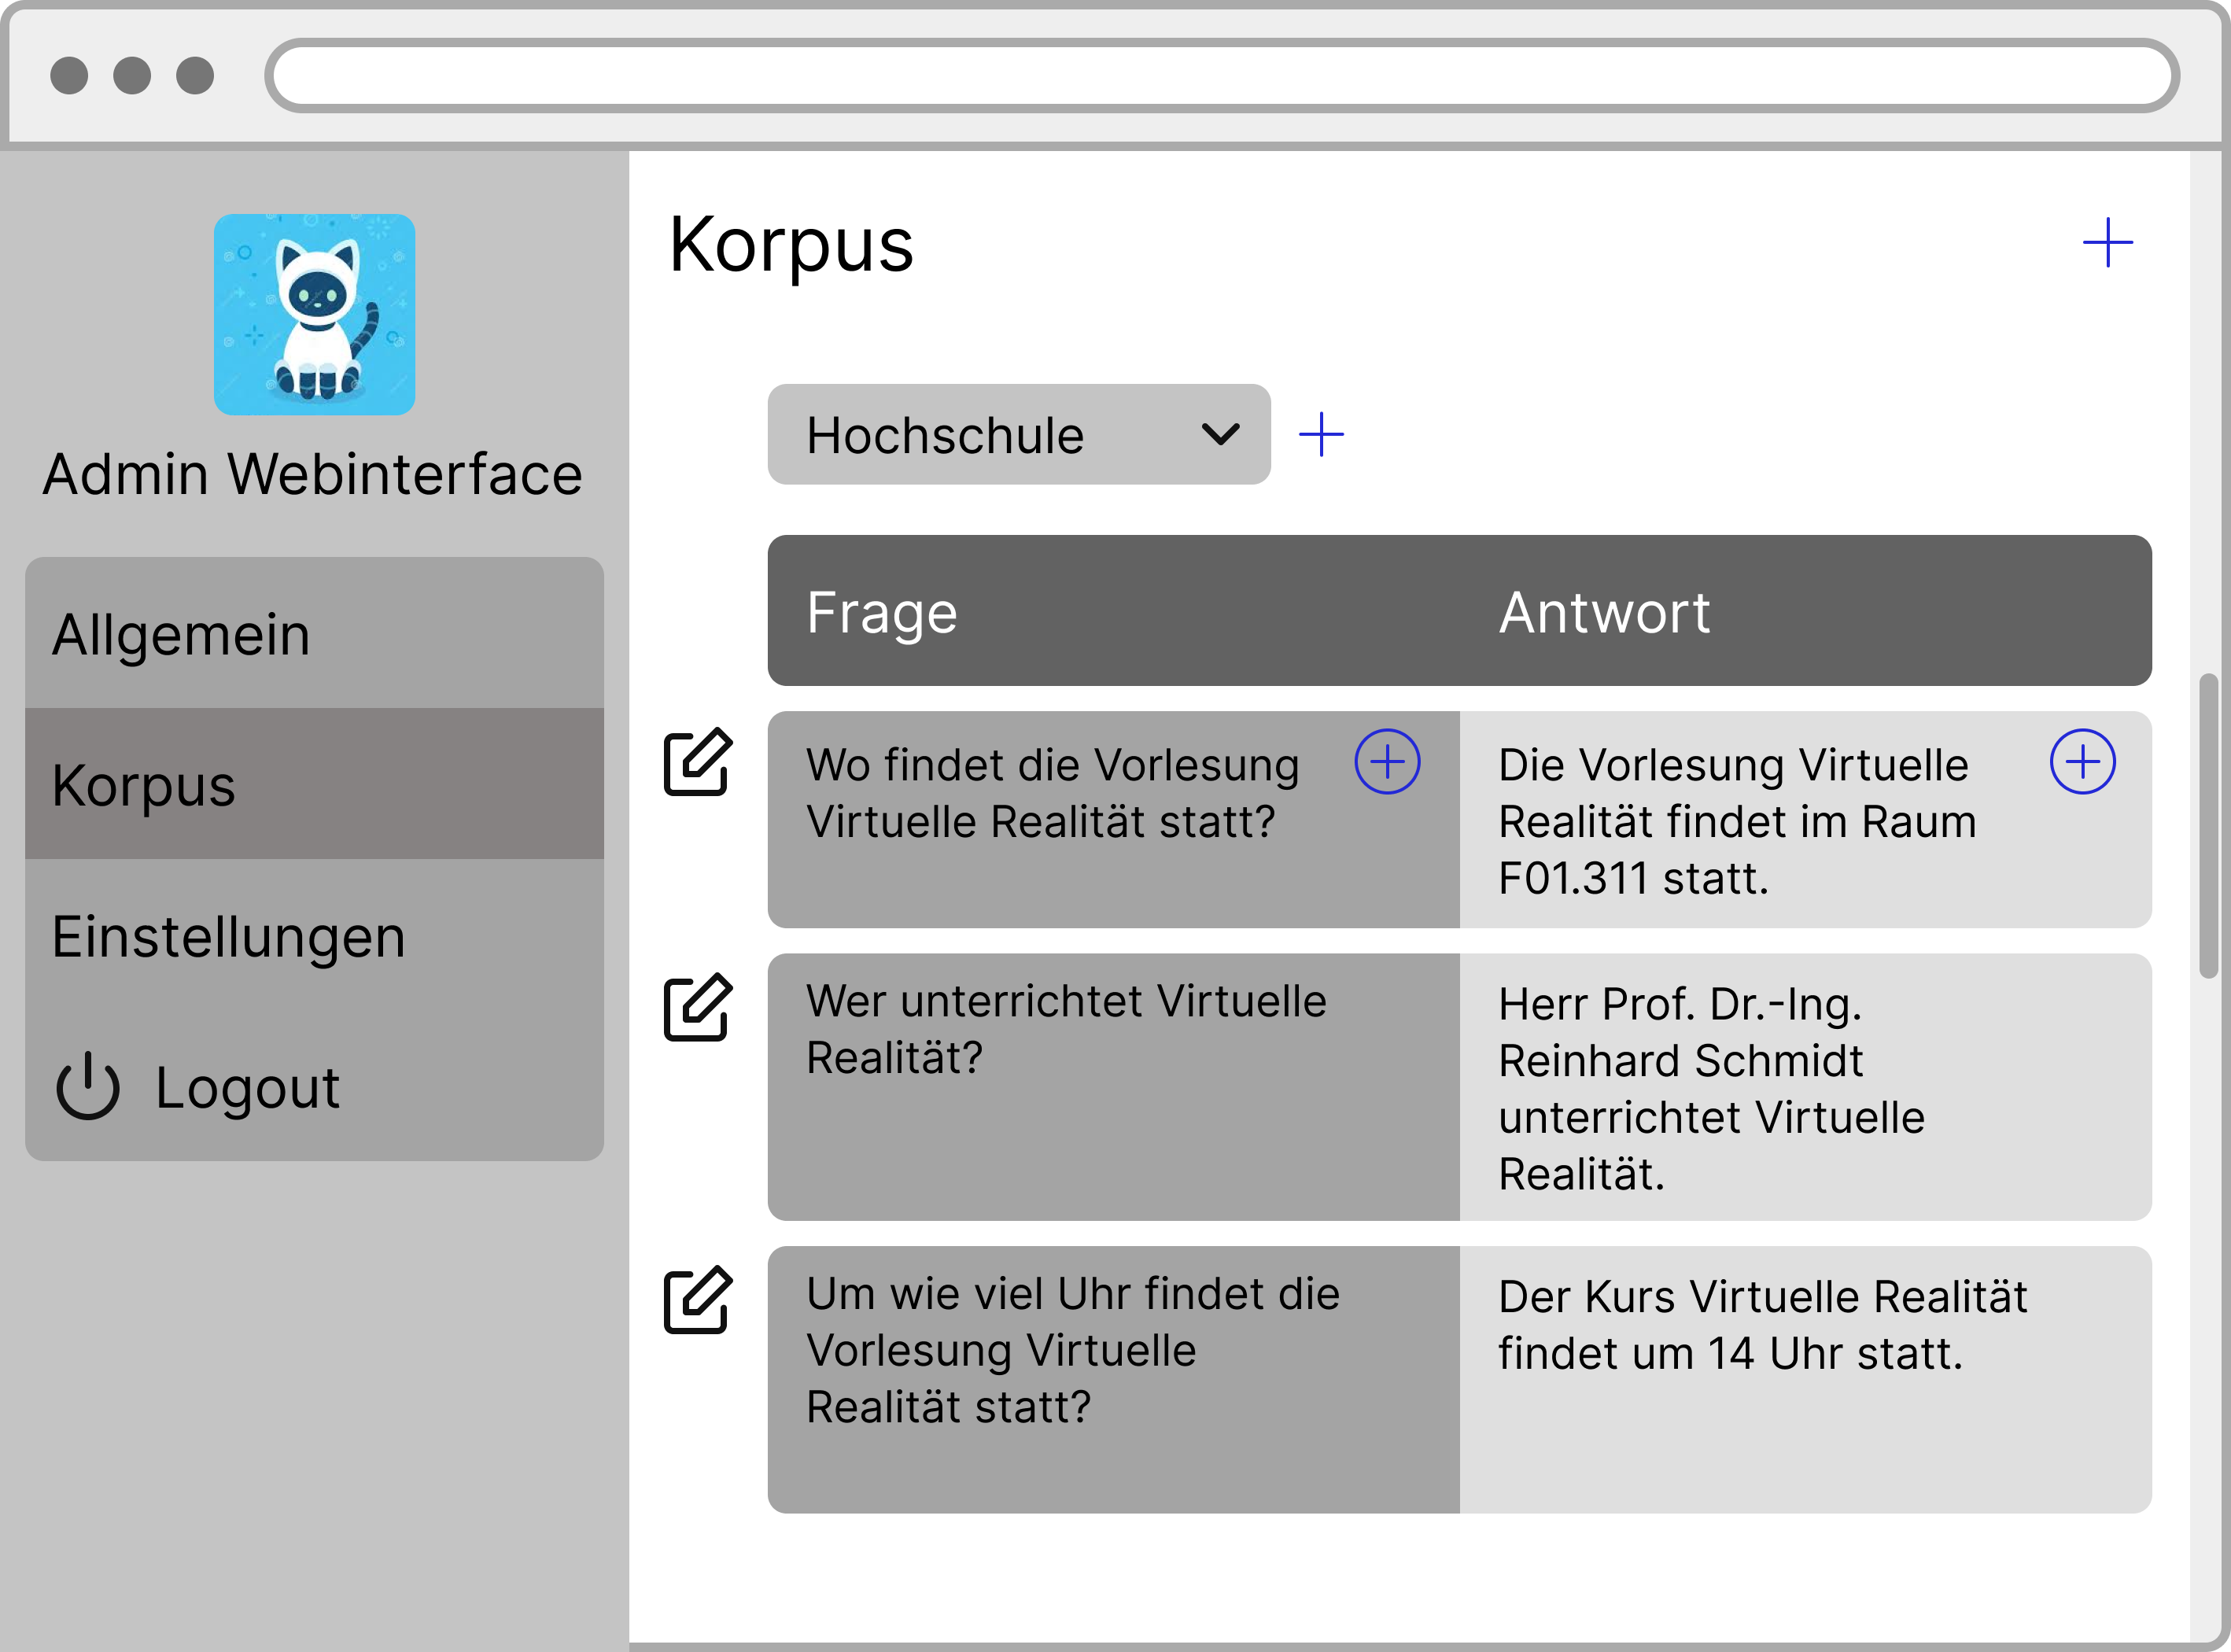
\includegraphics[width=1.0\textwidth]{bilder/new vers. UI Design/Korpus/Admin Interface 00.png}
    \caption{new version UI Design Admin-Interface Korpus 00}
    \label{fig:new version UI Design Admin-Interface Korpus 00}
\end{figure}
\noindent  \textbf{Admin Webinterface: Korpus 00} \newline
Im Korpus kann der Admin weitere Domänen, Fragen und Antworten einsehen.

\begin{figure}[H]
    \centering
    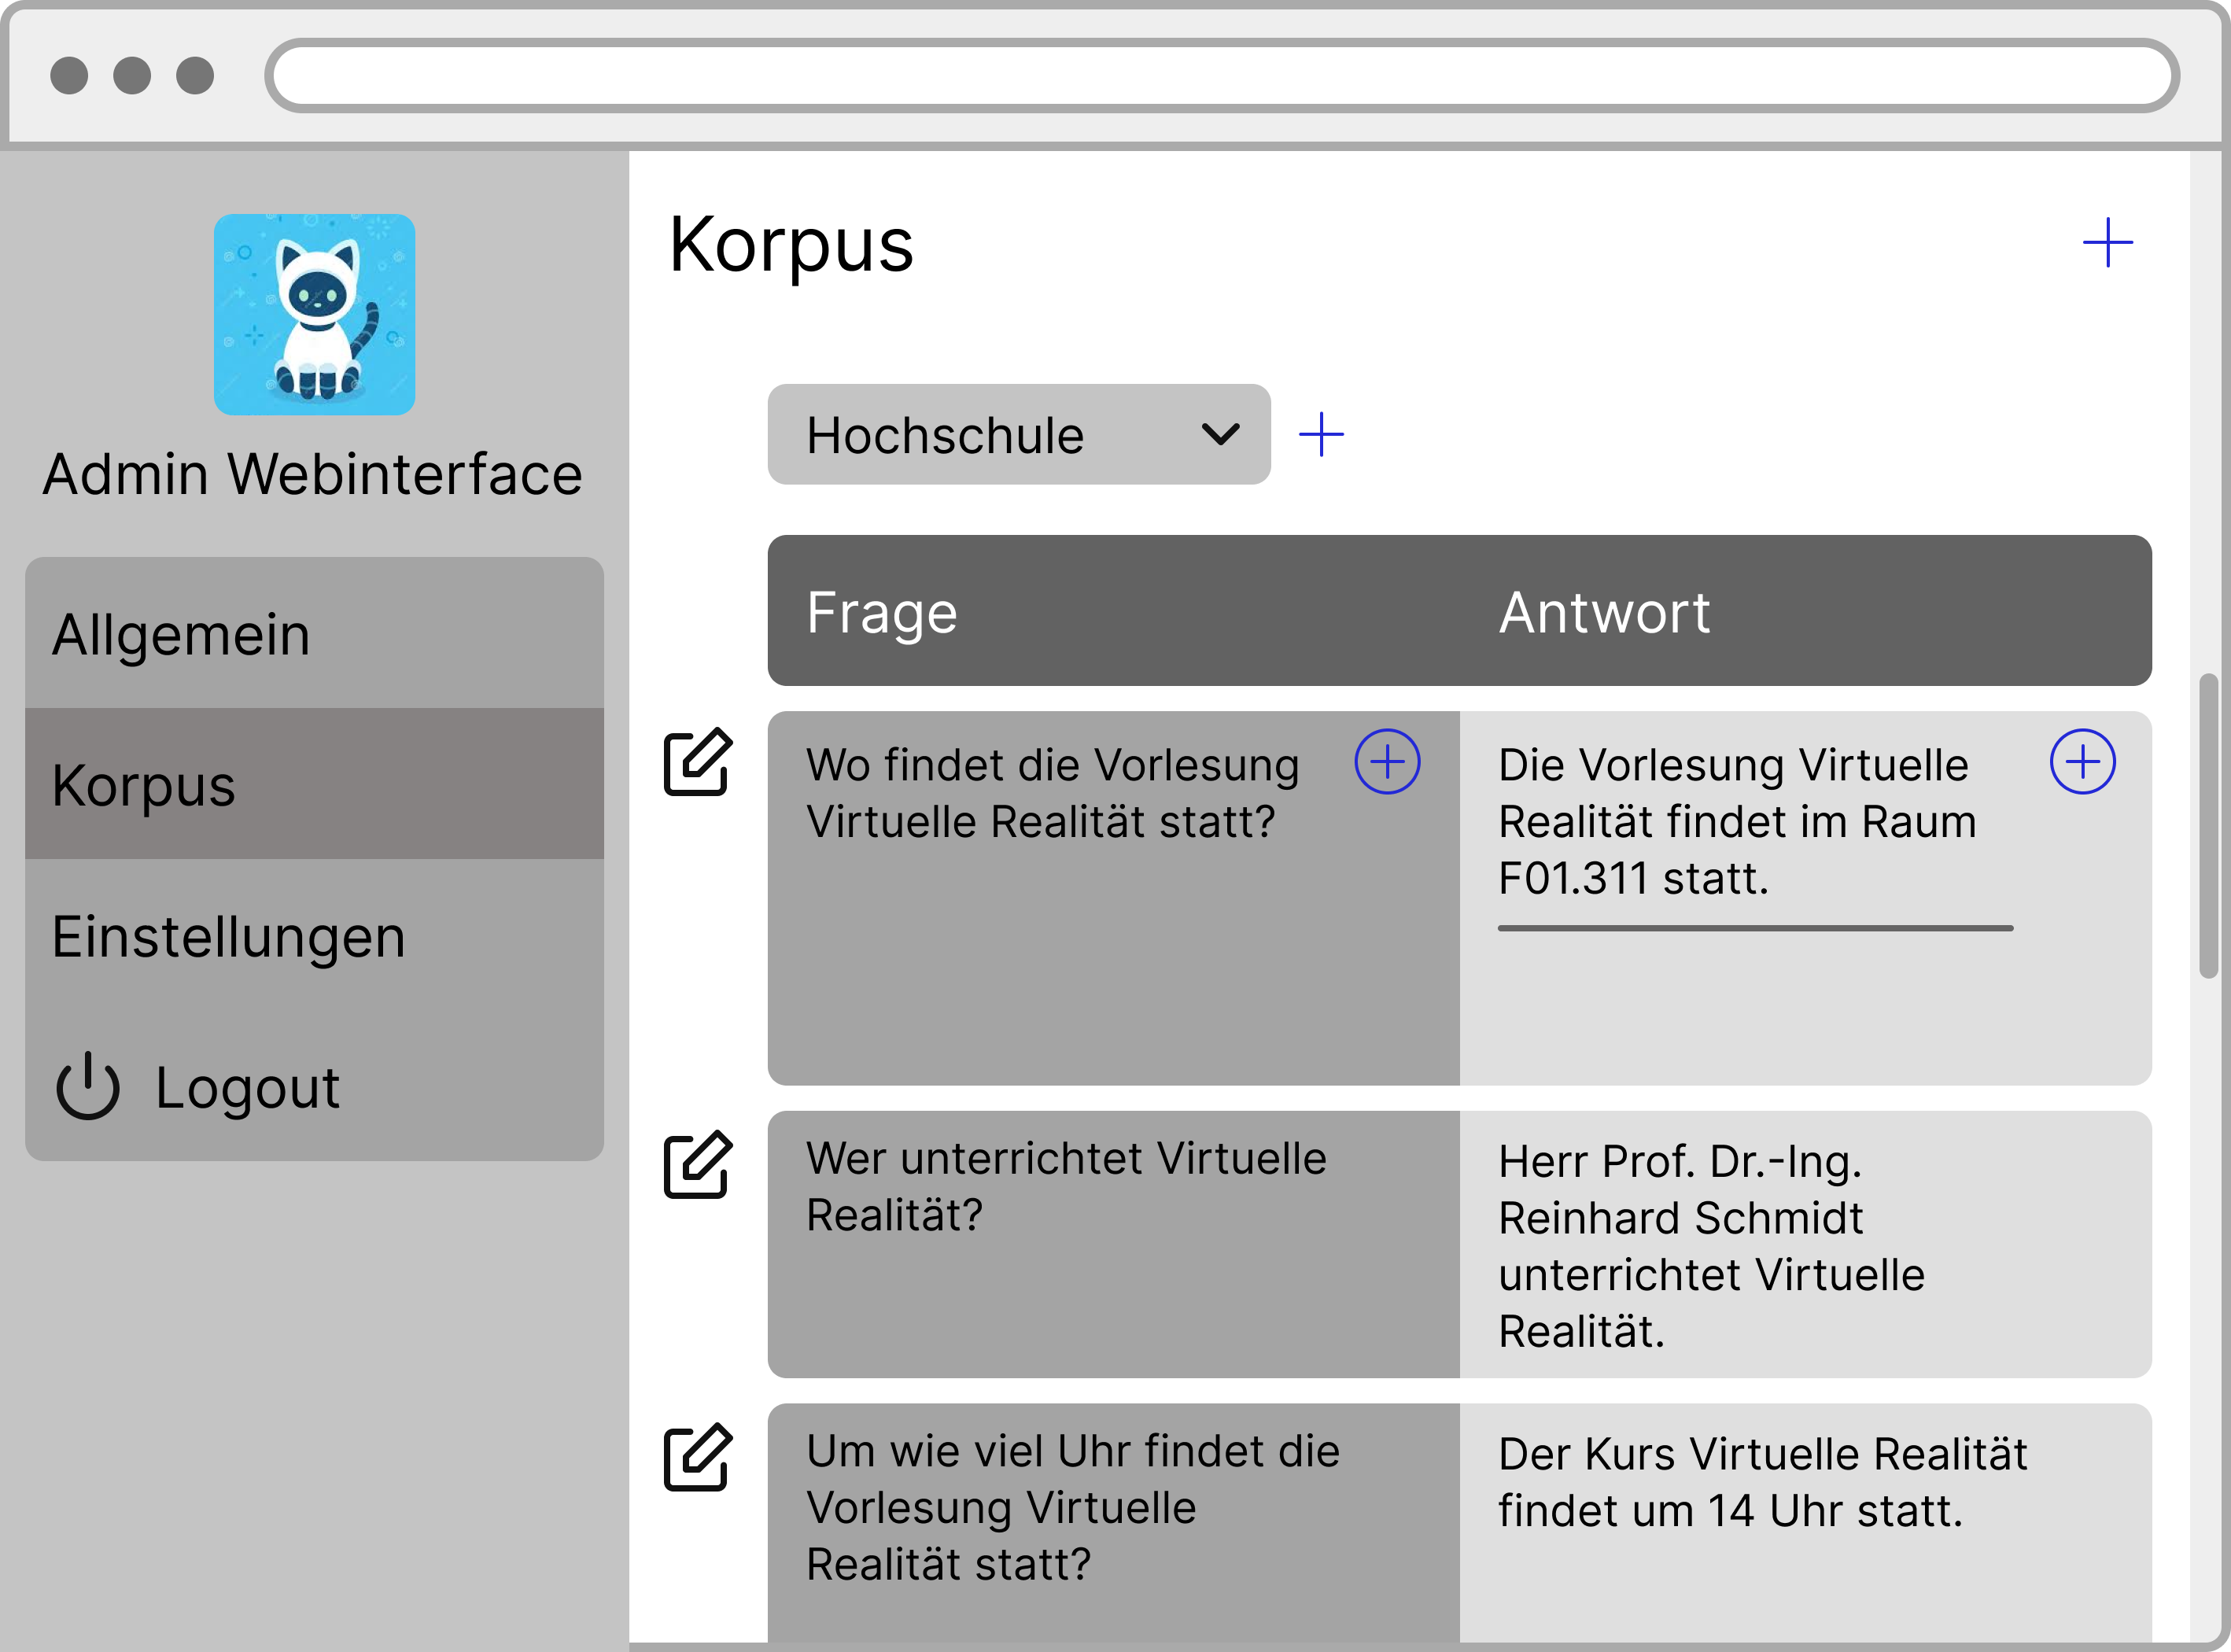
\includegraphics[width=1.0\textwidth]{bilder/new vers. UI Design/Korpus/Admin Interface 01.png}
    \caption{new version UI Design Admin-Interface Korpus 01}
    \label{fig:new version UI Design Admin-Interface Korpus 01}
\end{figure}
\noindent \textbf{Admin Webinterface: Korpus 01} \newline
Mit dem Editierbutton kann er Domänen, Fragen und Antworten hinzufügen und entfernen.

\begin{figure}[H]
    \centering
    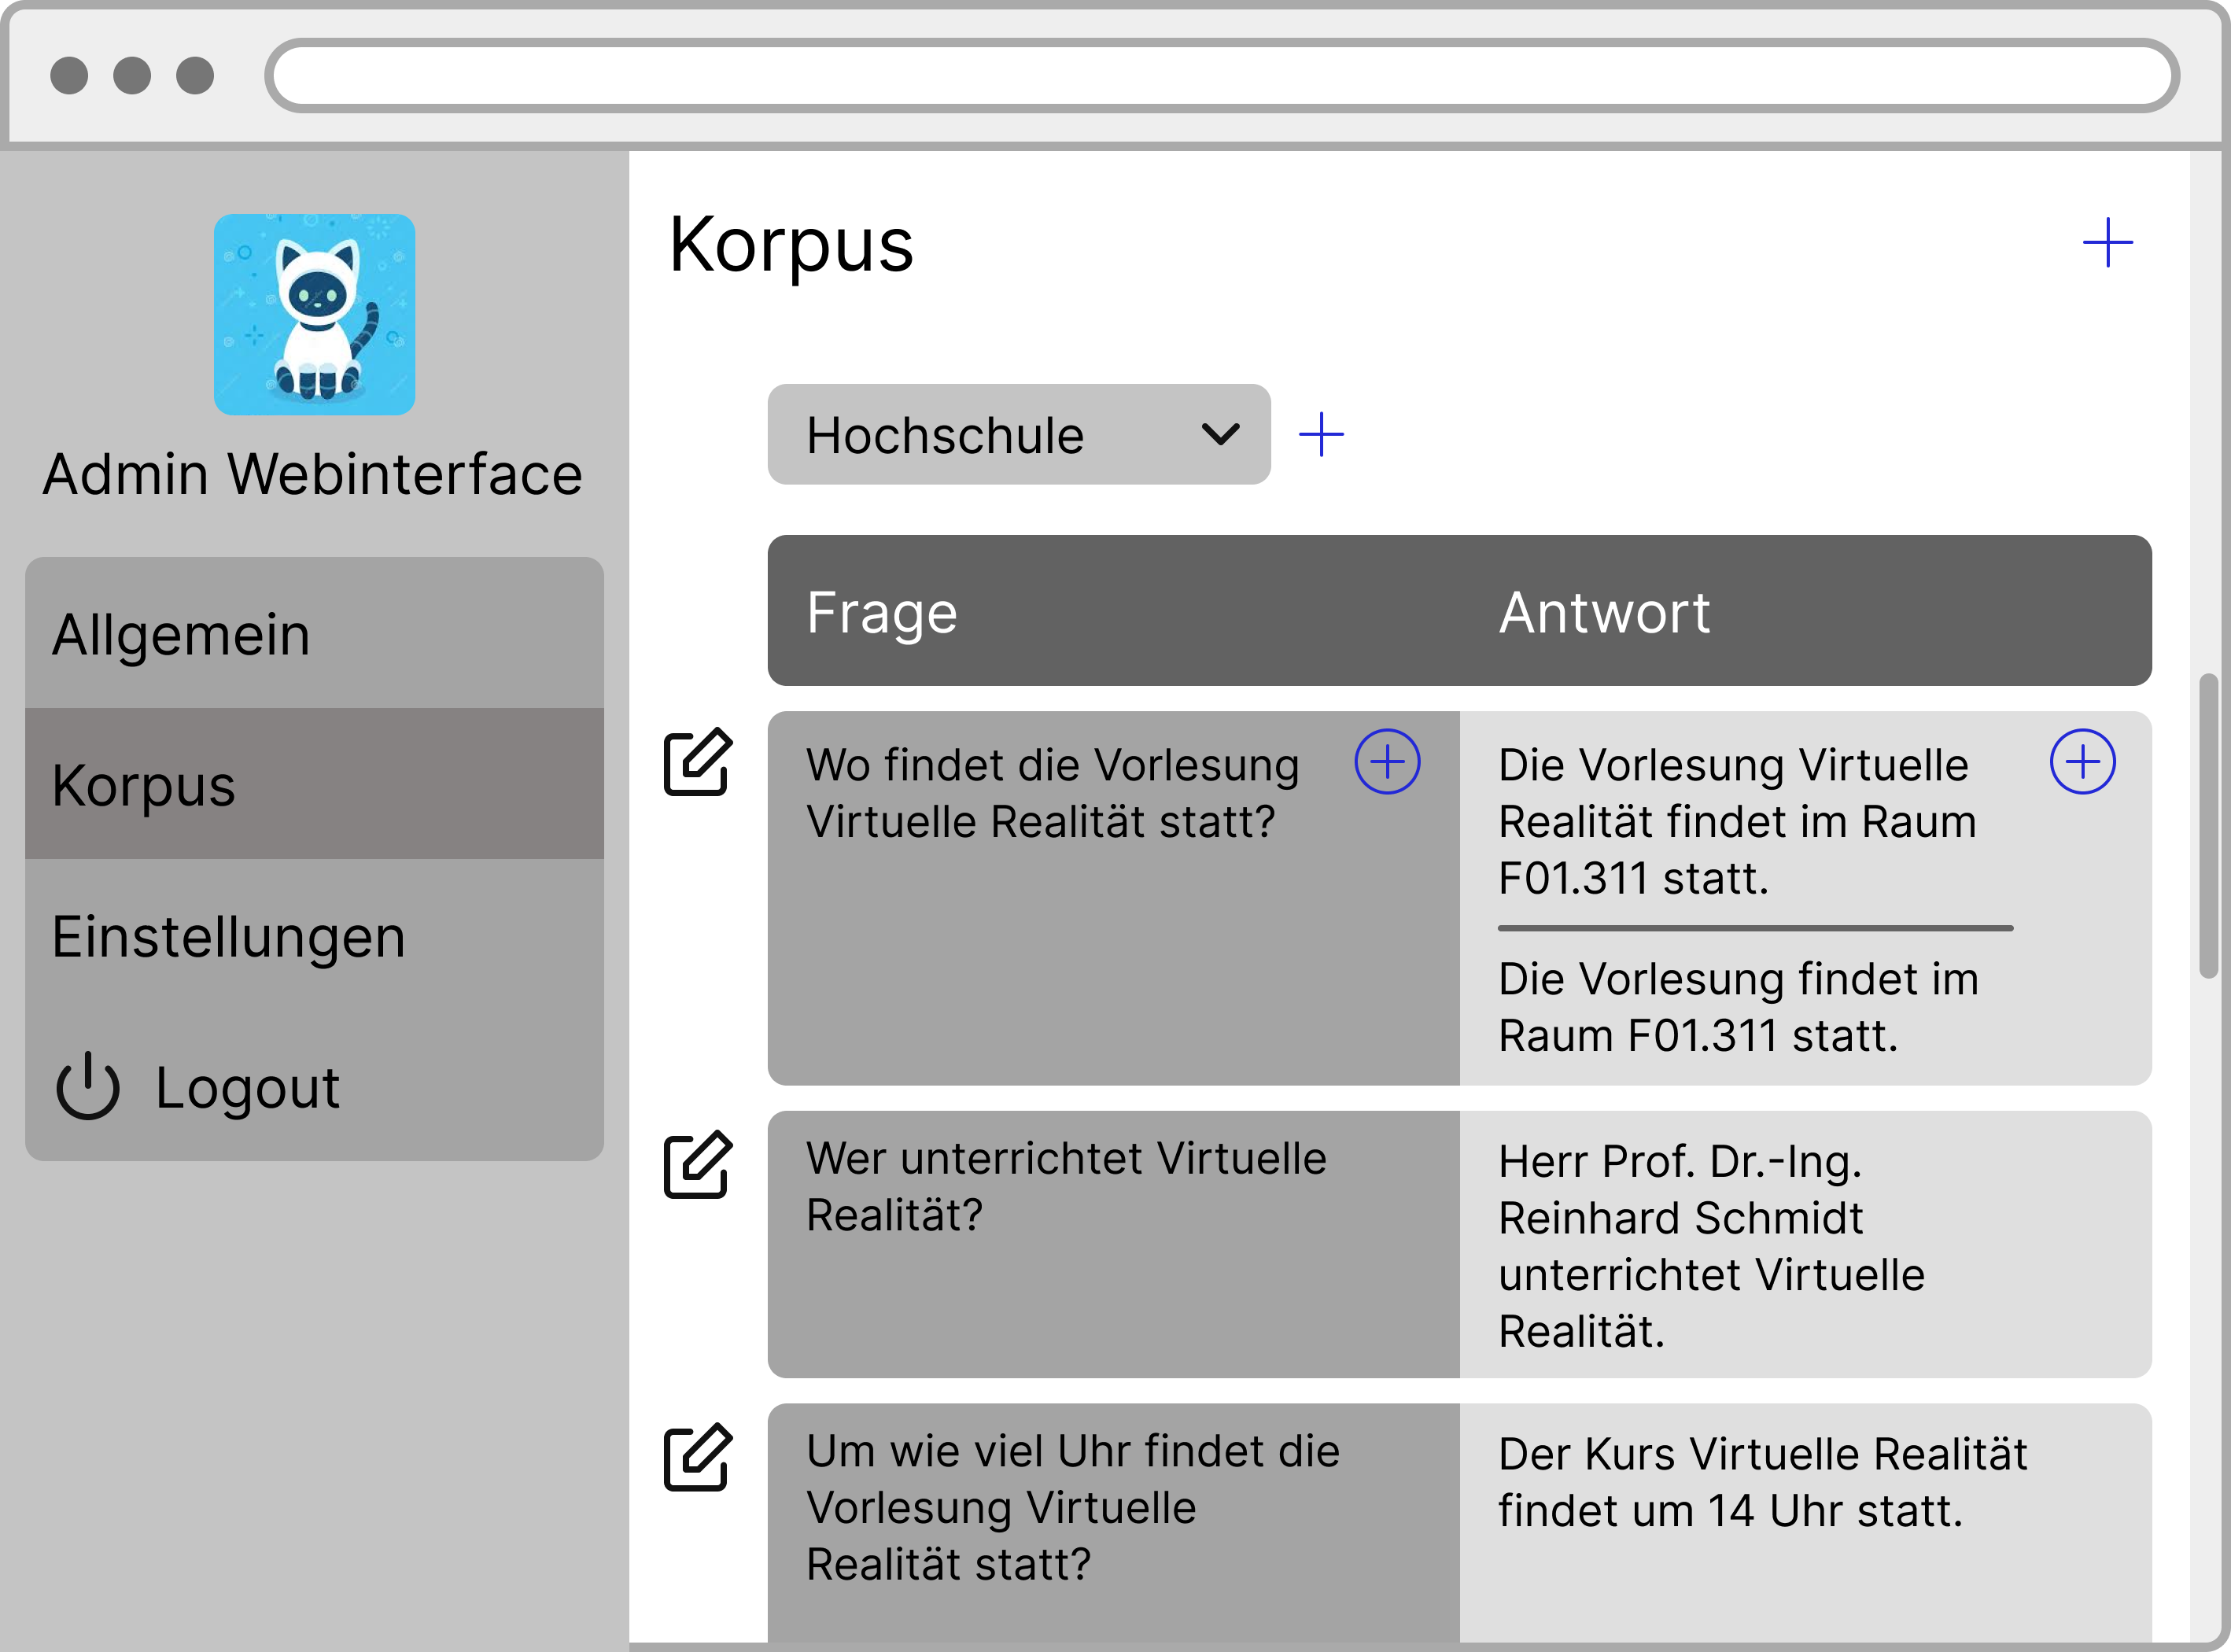
\includegraphics[width=1.0\textwidth]{bilder/new vers. UI Design/Korpus/Admin Interface 02.png}
    \caption{new version UI Design Admin-Interface Korpus 02}
    \label{fig:new version UI Design Admin-Interface Korpus 02}
\end{figure}
\noindent \textbf{Admin Webinterface: Korpus 02} \newline
So kann man wie im Beispiel eine weitere Antwort zu der Frage: "Wo findet die Vorlesung Virtuelle
Realität statt?", hinzufügen.

\begin{figure}[H]
    \centering
    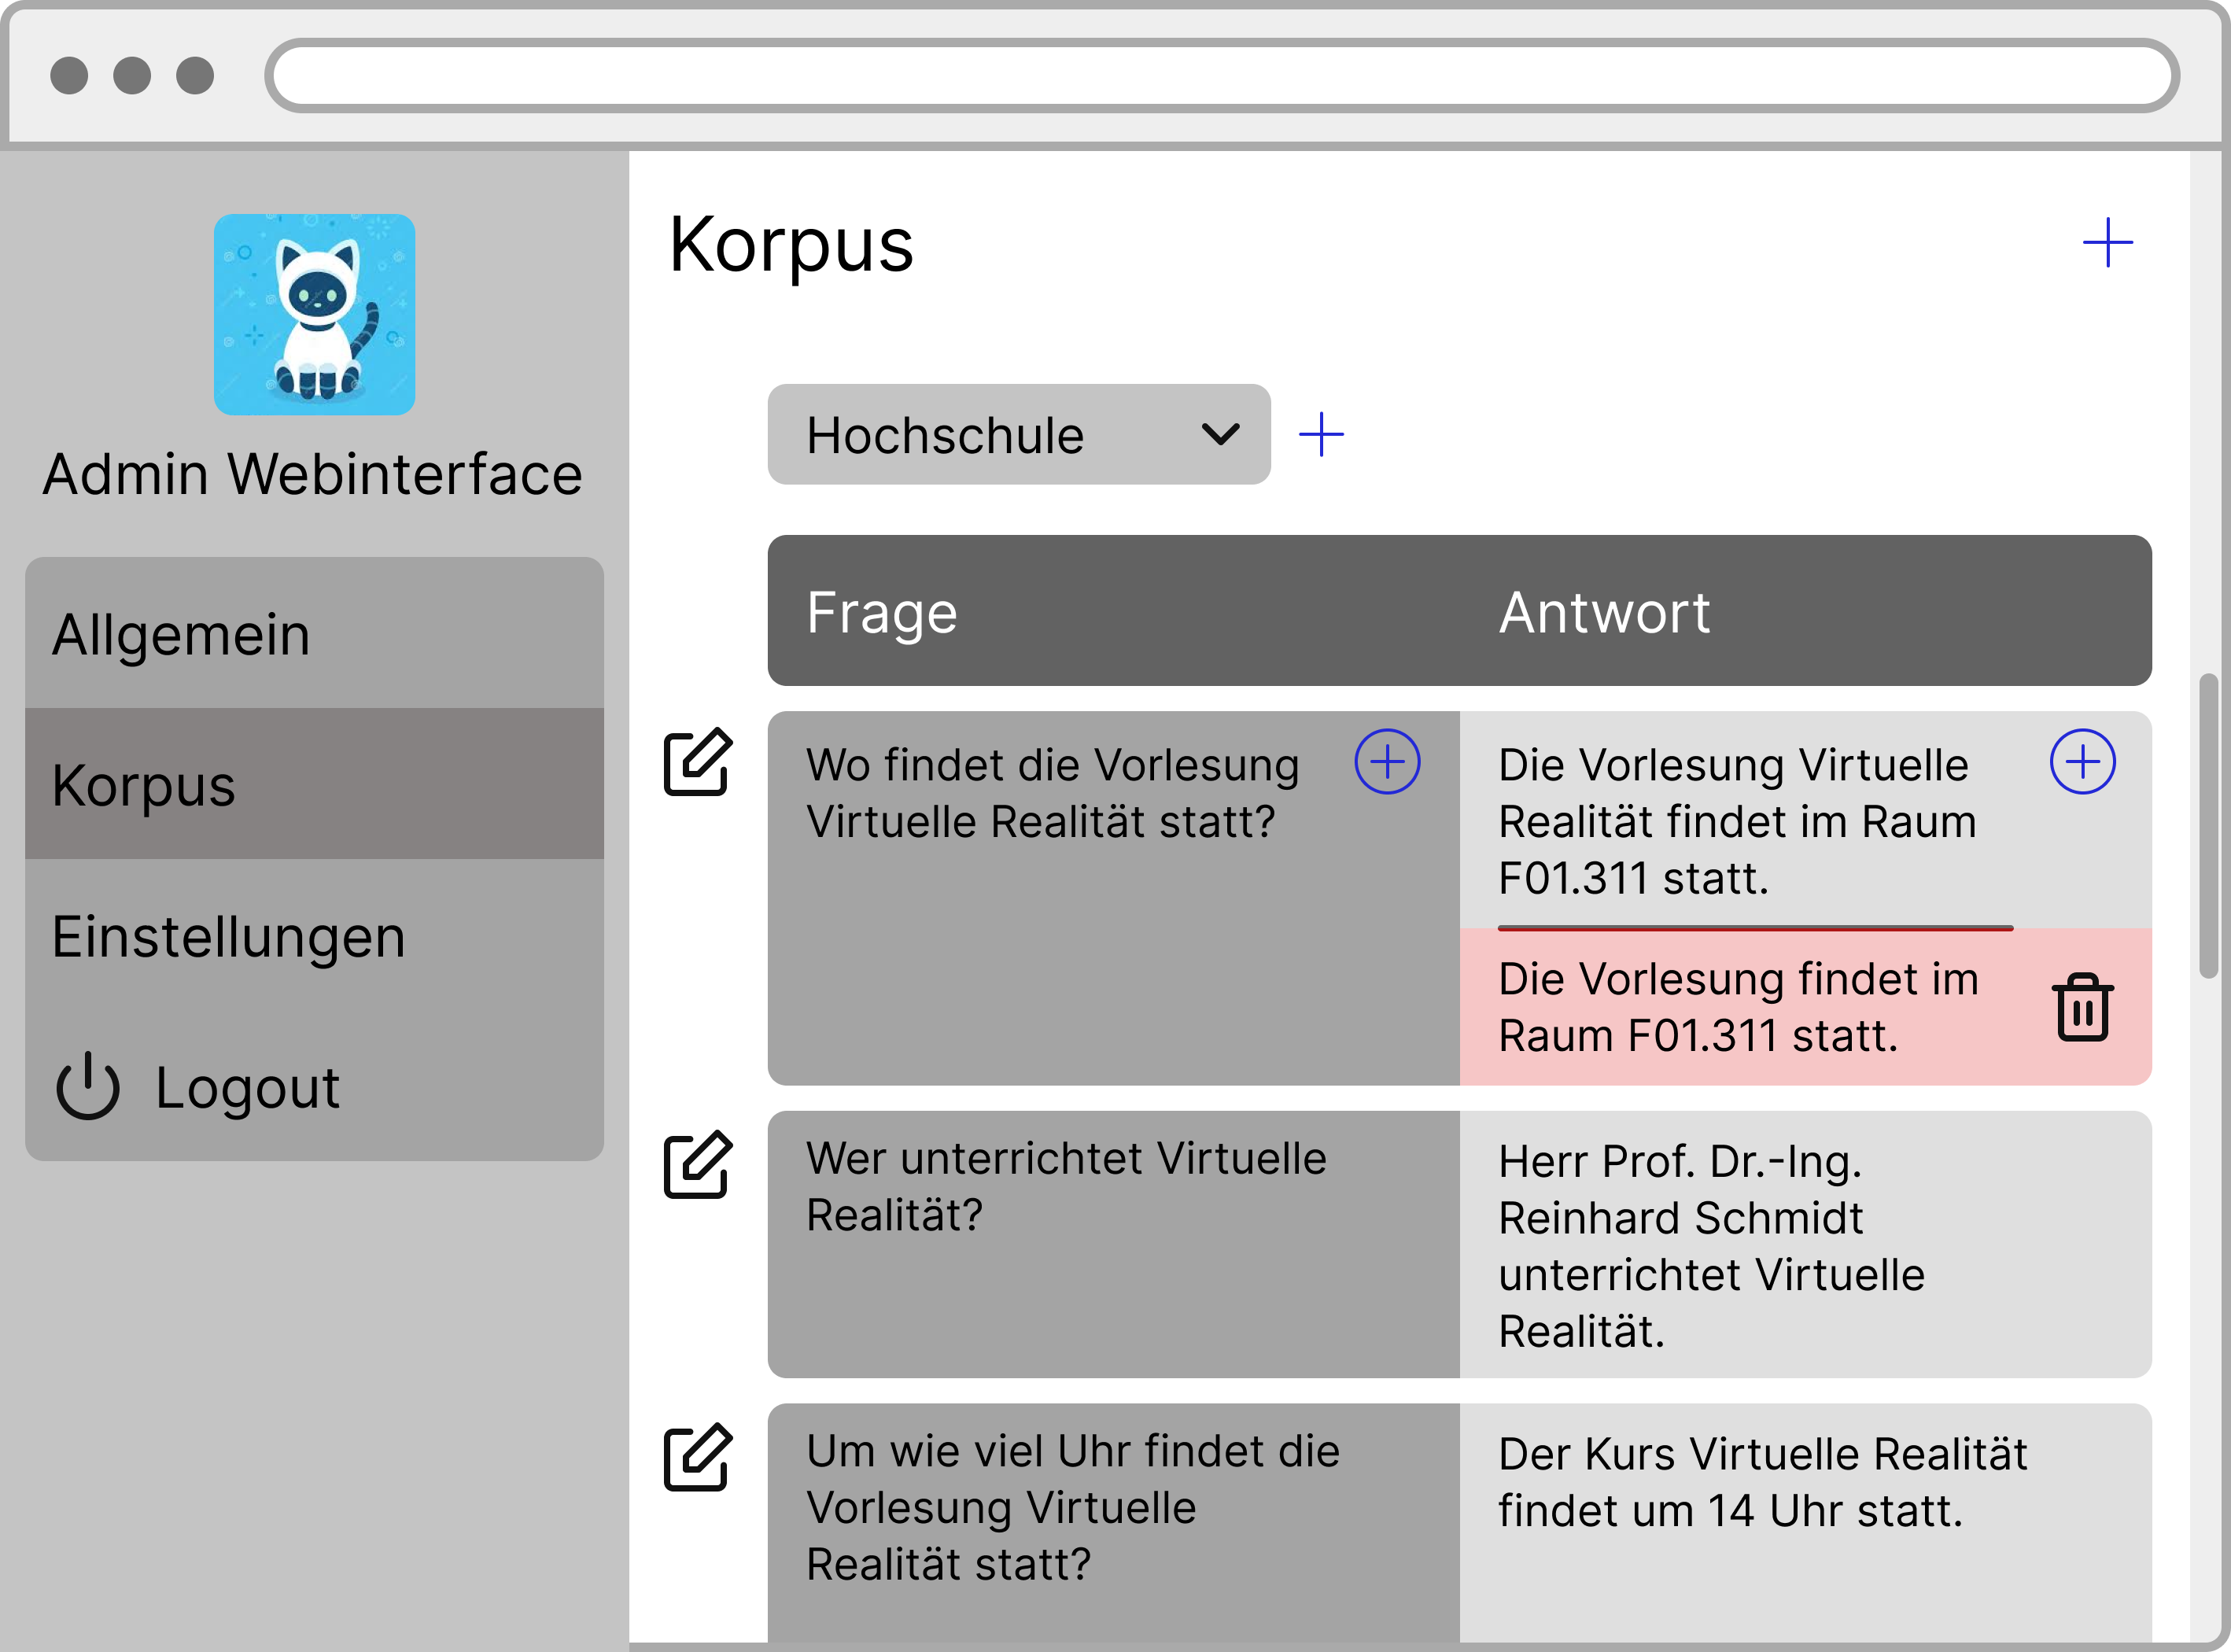
\includegraphics[width=1.0\textwidth]{bilder/new vers. UI Design/Korpus/Admin Interface 03.png}
    \caption{new version UI Design Admin-Interface Korpus 03}
    \label{fig:new version UI Design Admin-Interface Korpus 03}
\end{figure}
\noindent \textbf{Admin Webinterface: Korpus 03} \newline
Natürlich kann man auch die hnzugefügte Antwort entfernen. Man klickt auf das Feld und das Feld erscheint rötlich und ein
Mülleimersymbol entsteht. Wenn man jetzt auf das Eimer-Symbol klickt kann man die
Antwort löschen.

\begin{figure}[H]
    \centering
    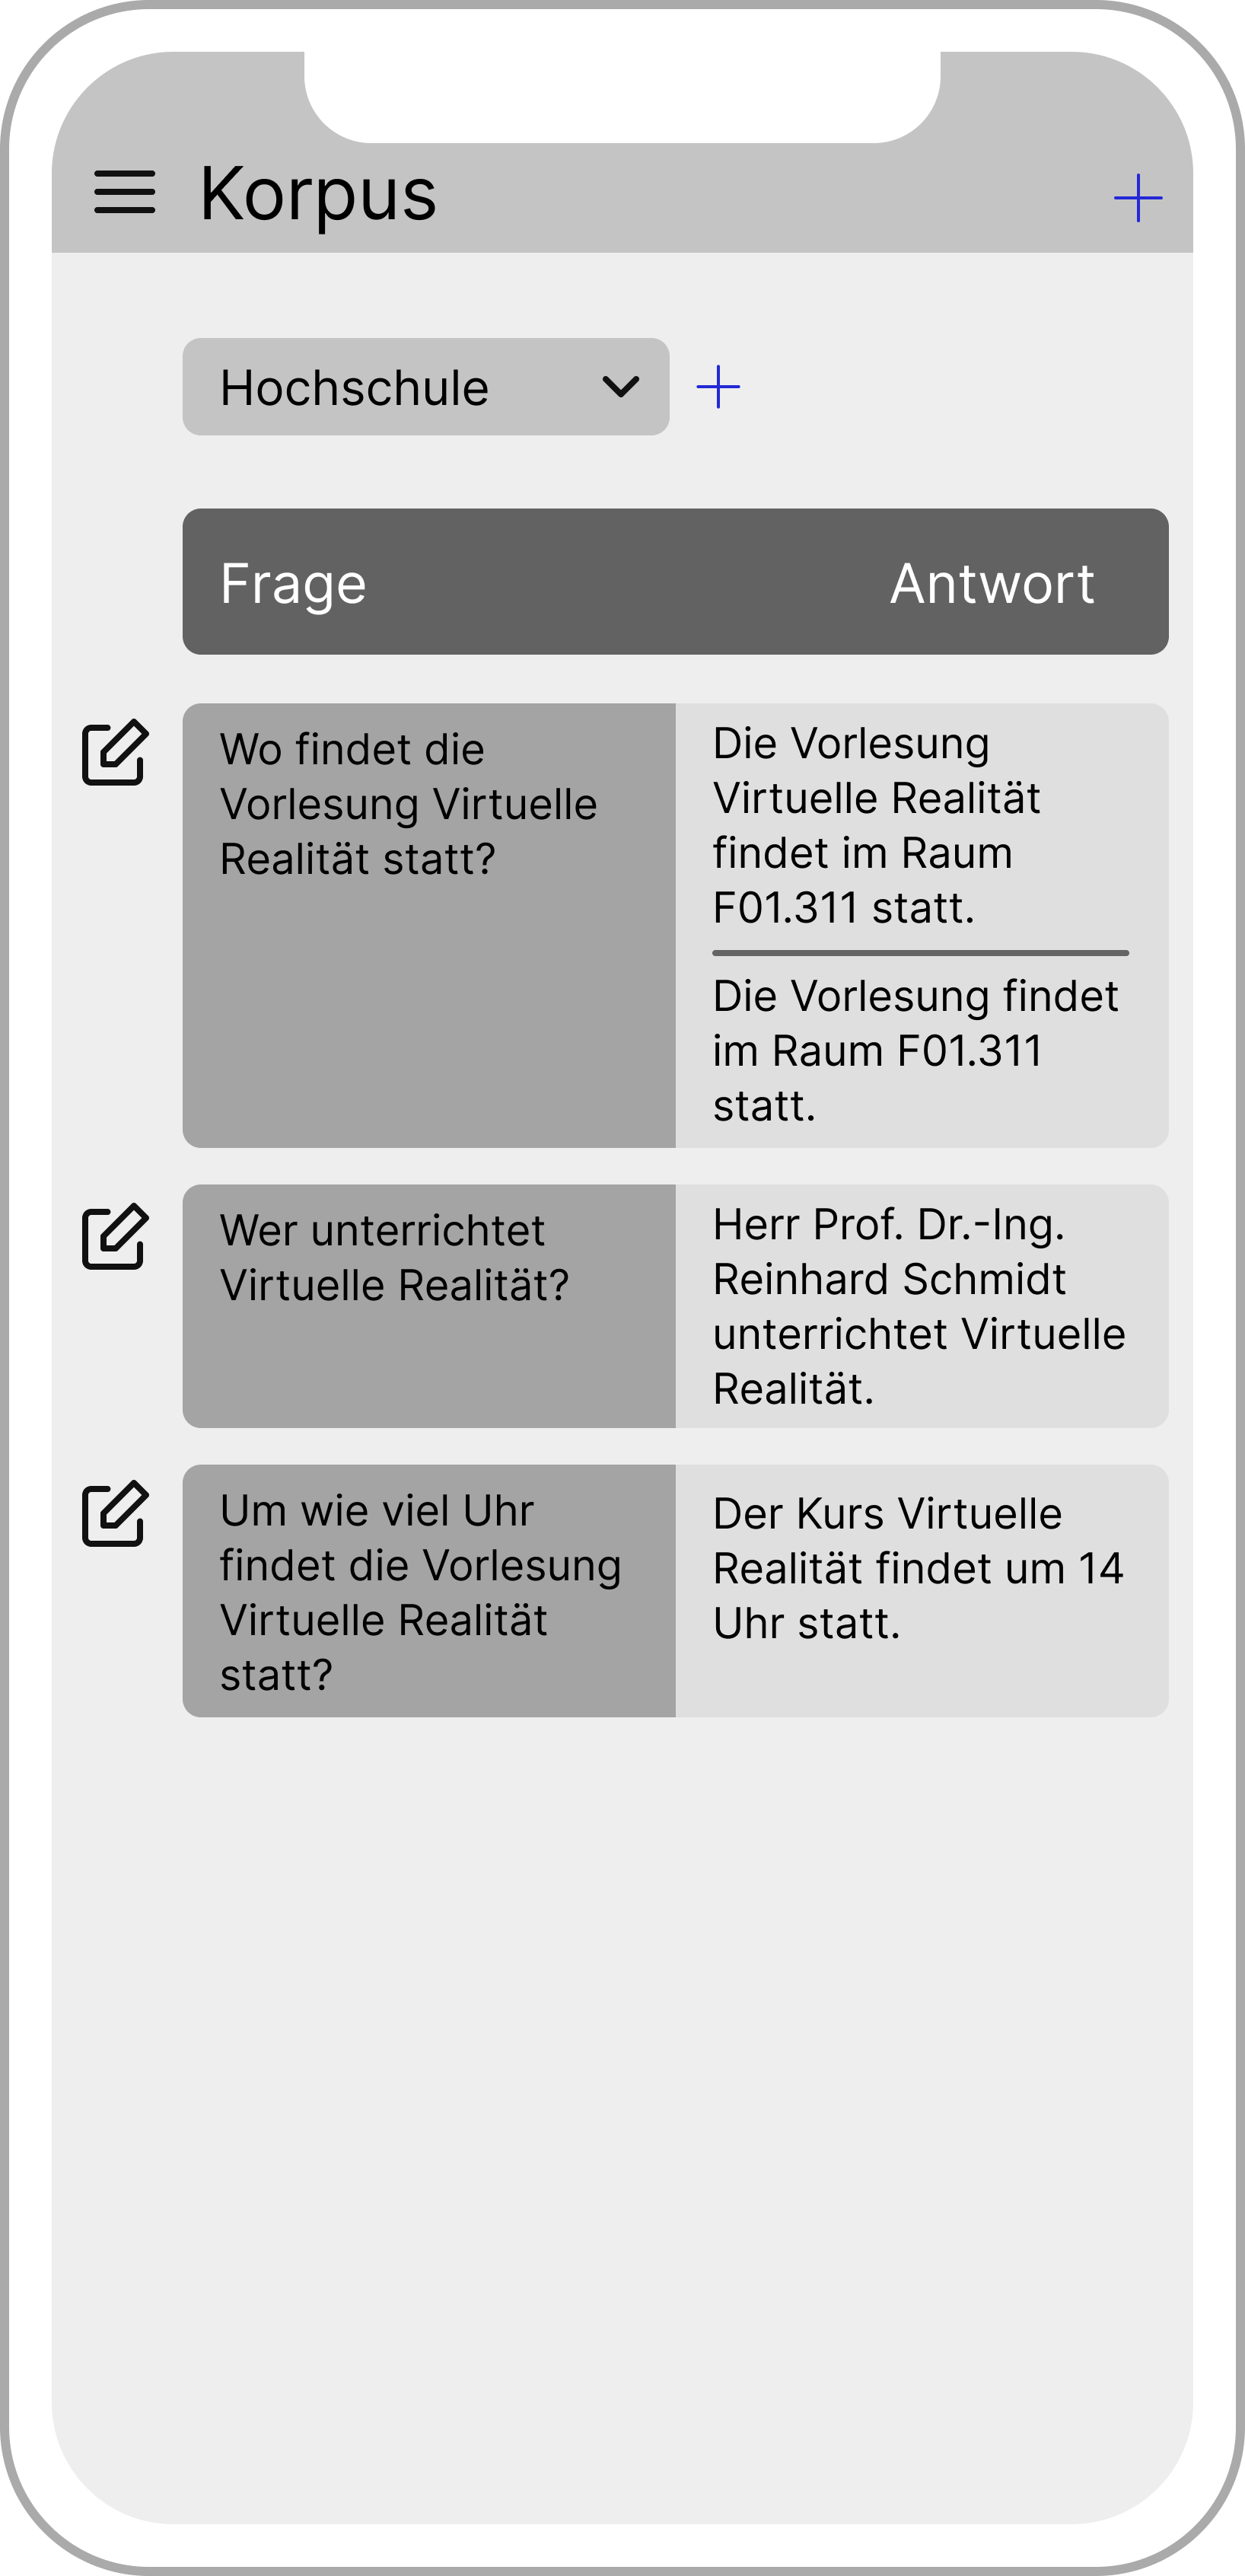
\includegraphics[width=0.5\textwidth]{bilder/new vers. UI Design/Korpus/iPhone X Korpus I.png}
    \caption{new version UI Design Admin-Interface Korpus mobile version}
    \label{fig:new version UI Design Admin-Interface Korpus mobile version}
\end{figure}
\noindent \textbf{Admin Webinterface mobil: Korpus} \newline
In der mobilen Version des Korpuses kann man die Elemente genauso editieren wie im Webbrowser.

\subsubsection{Version 2 Admin Interface Einstellungen}
Hier werden die neueren Versionen des UI Designs für das Admin-Interface Einstellungen vorgestellt

\begin{figure}[H]
    \centering
    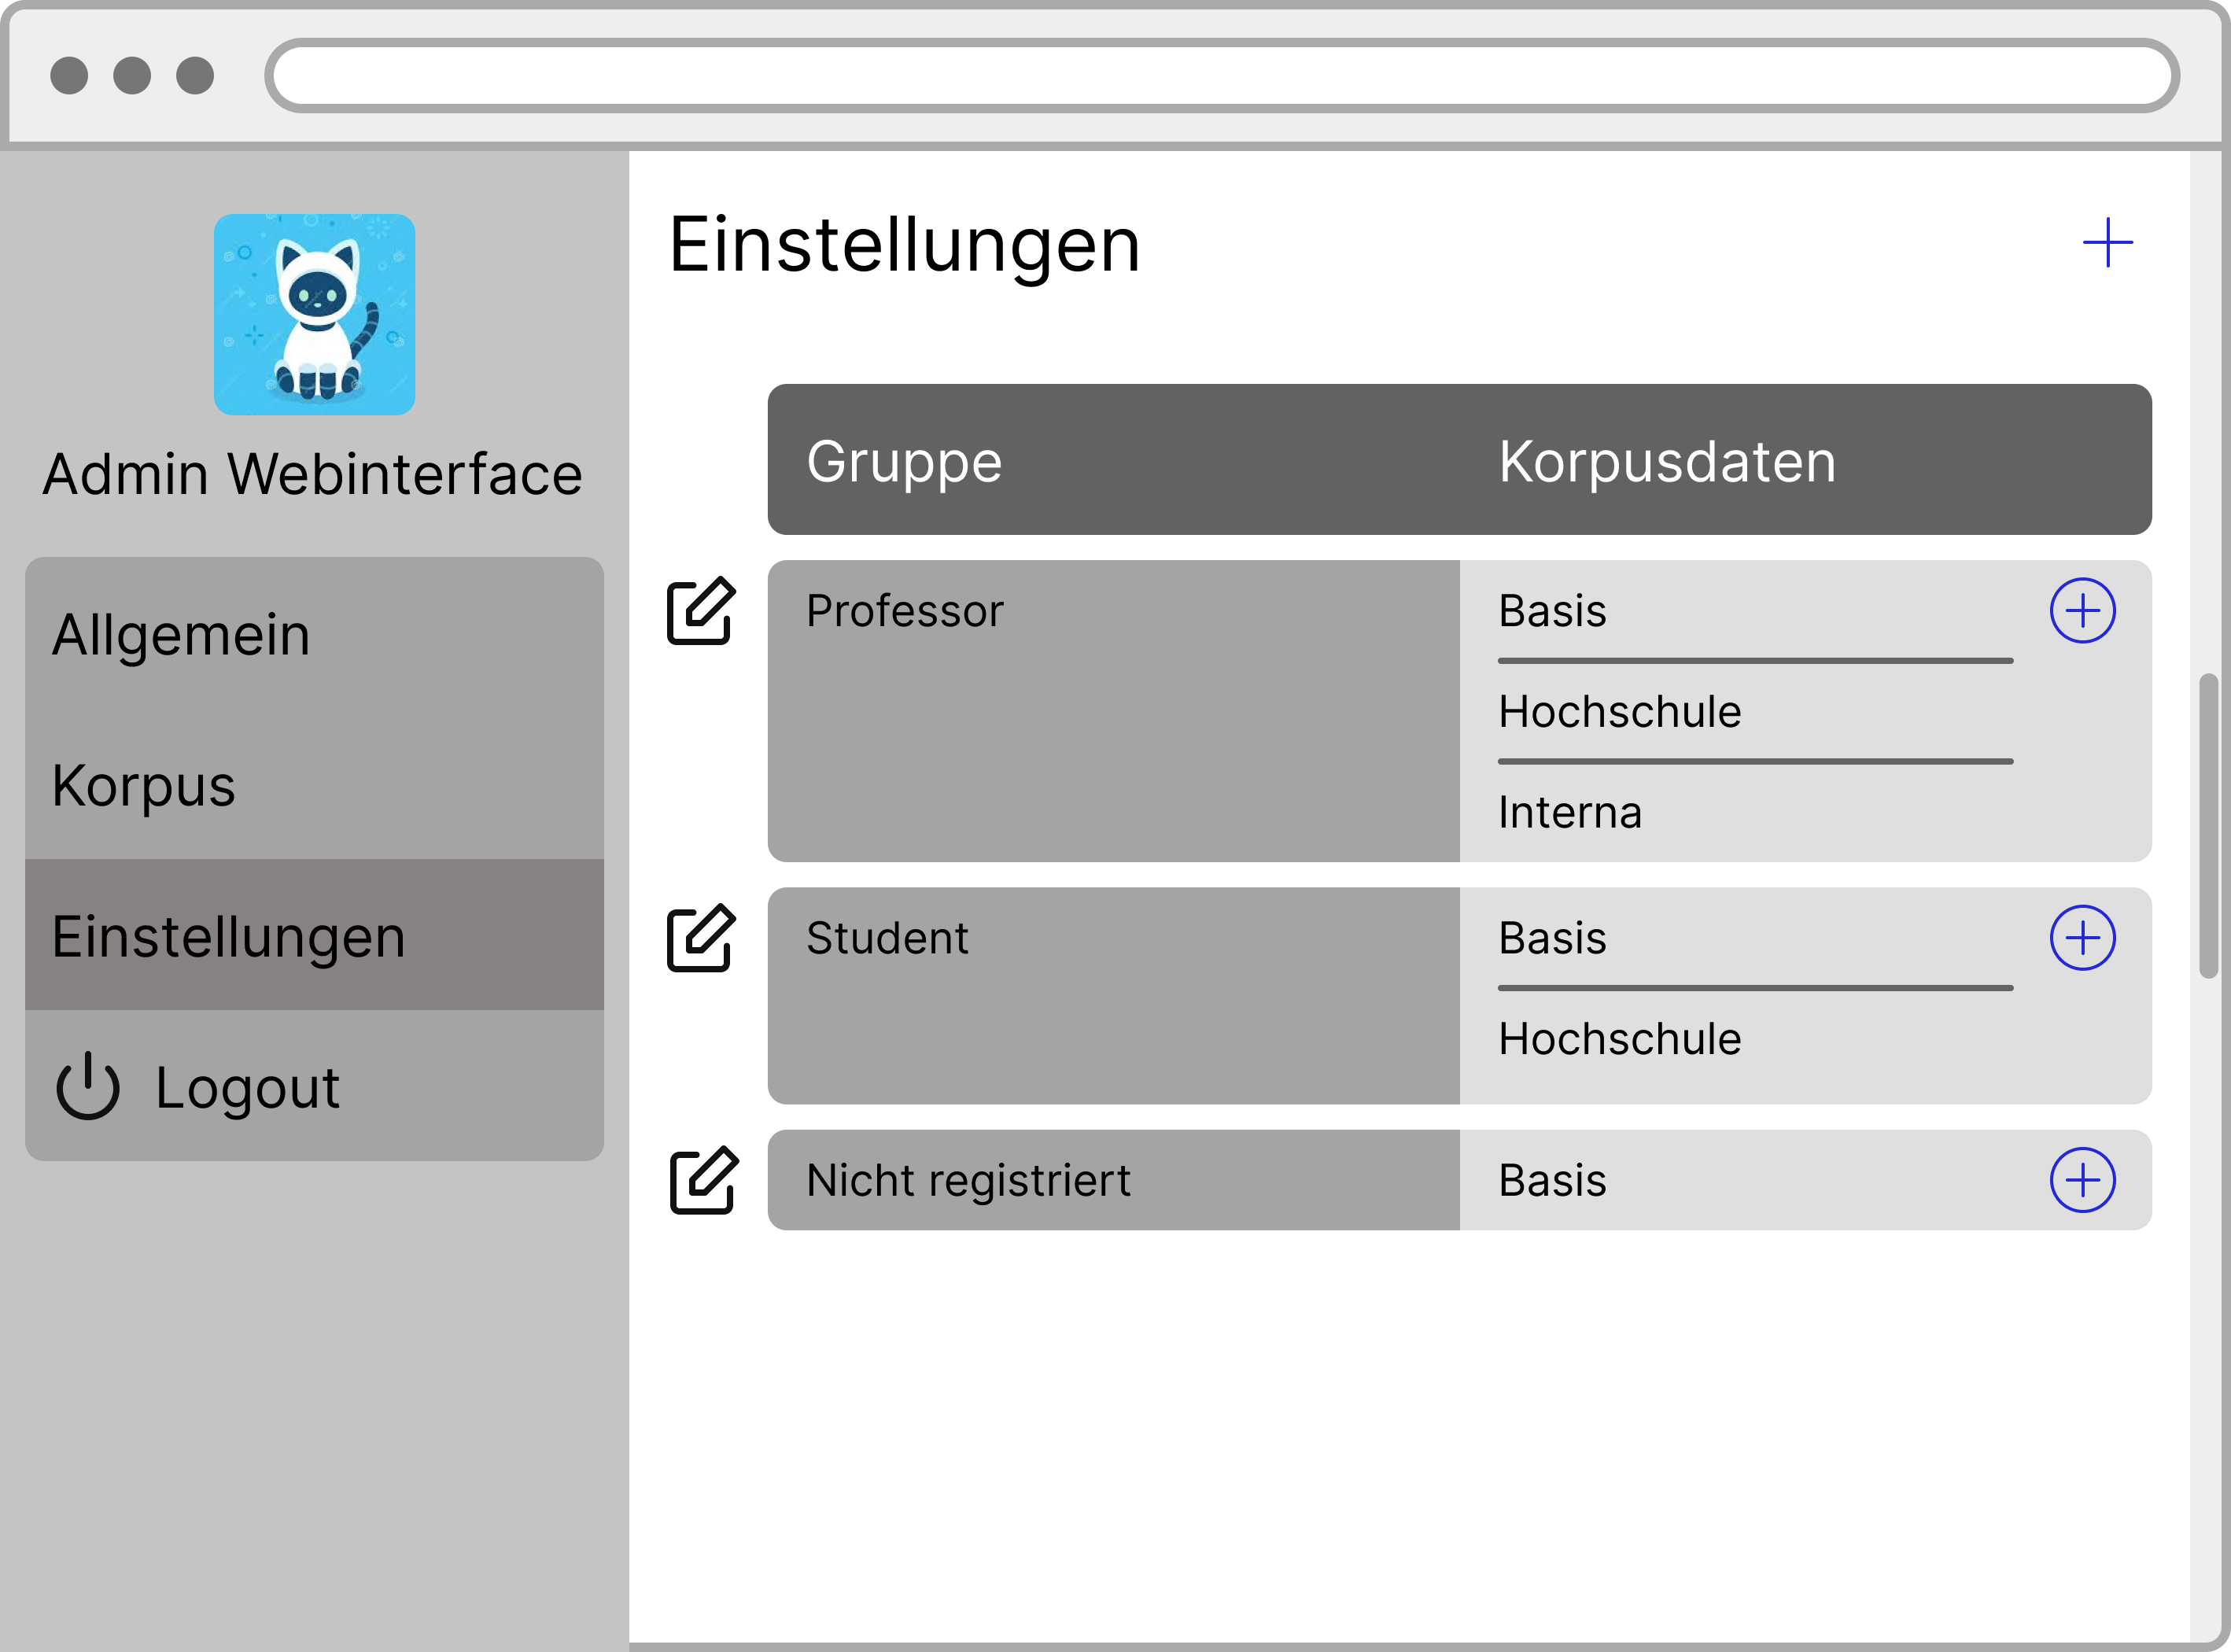
\includegraphics[width=1.0\textwidth]{bilder/new vers. UI Design/Einstellungen/Einstellungen (1).png}
    \caption{new version UI Design Admin-Interface Einstellungen}
    \label{fig:new version UI Design Admin-Interface Einstellungen}
\end{figure}
\noindent \textbf{Admin Webinterface: Einstellungen} \newline
In Einstellungen kann der Admin seine Gruppen einsehen, hinzufügen und entfernen. Er kann auch
die dazugehörenden Korpusdaten sehen und bearbeiten. In den Korpusdaten sind die Domänen der jeweilligen Gruppe eingetragen.

\begin{figure}[H]
    \centering
    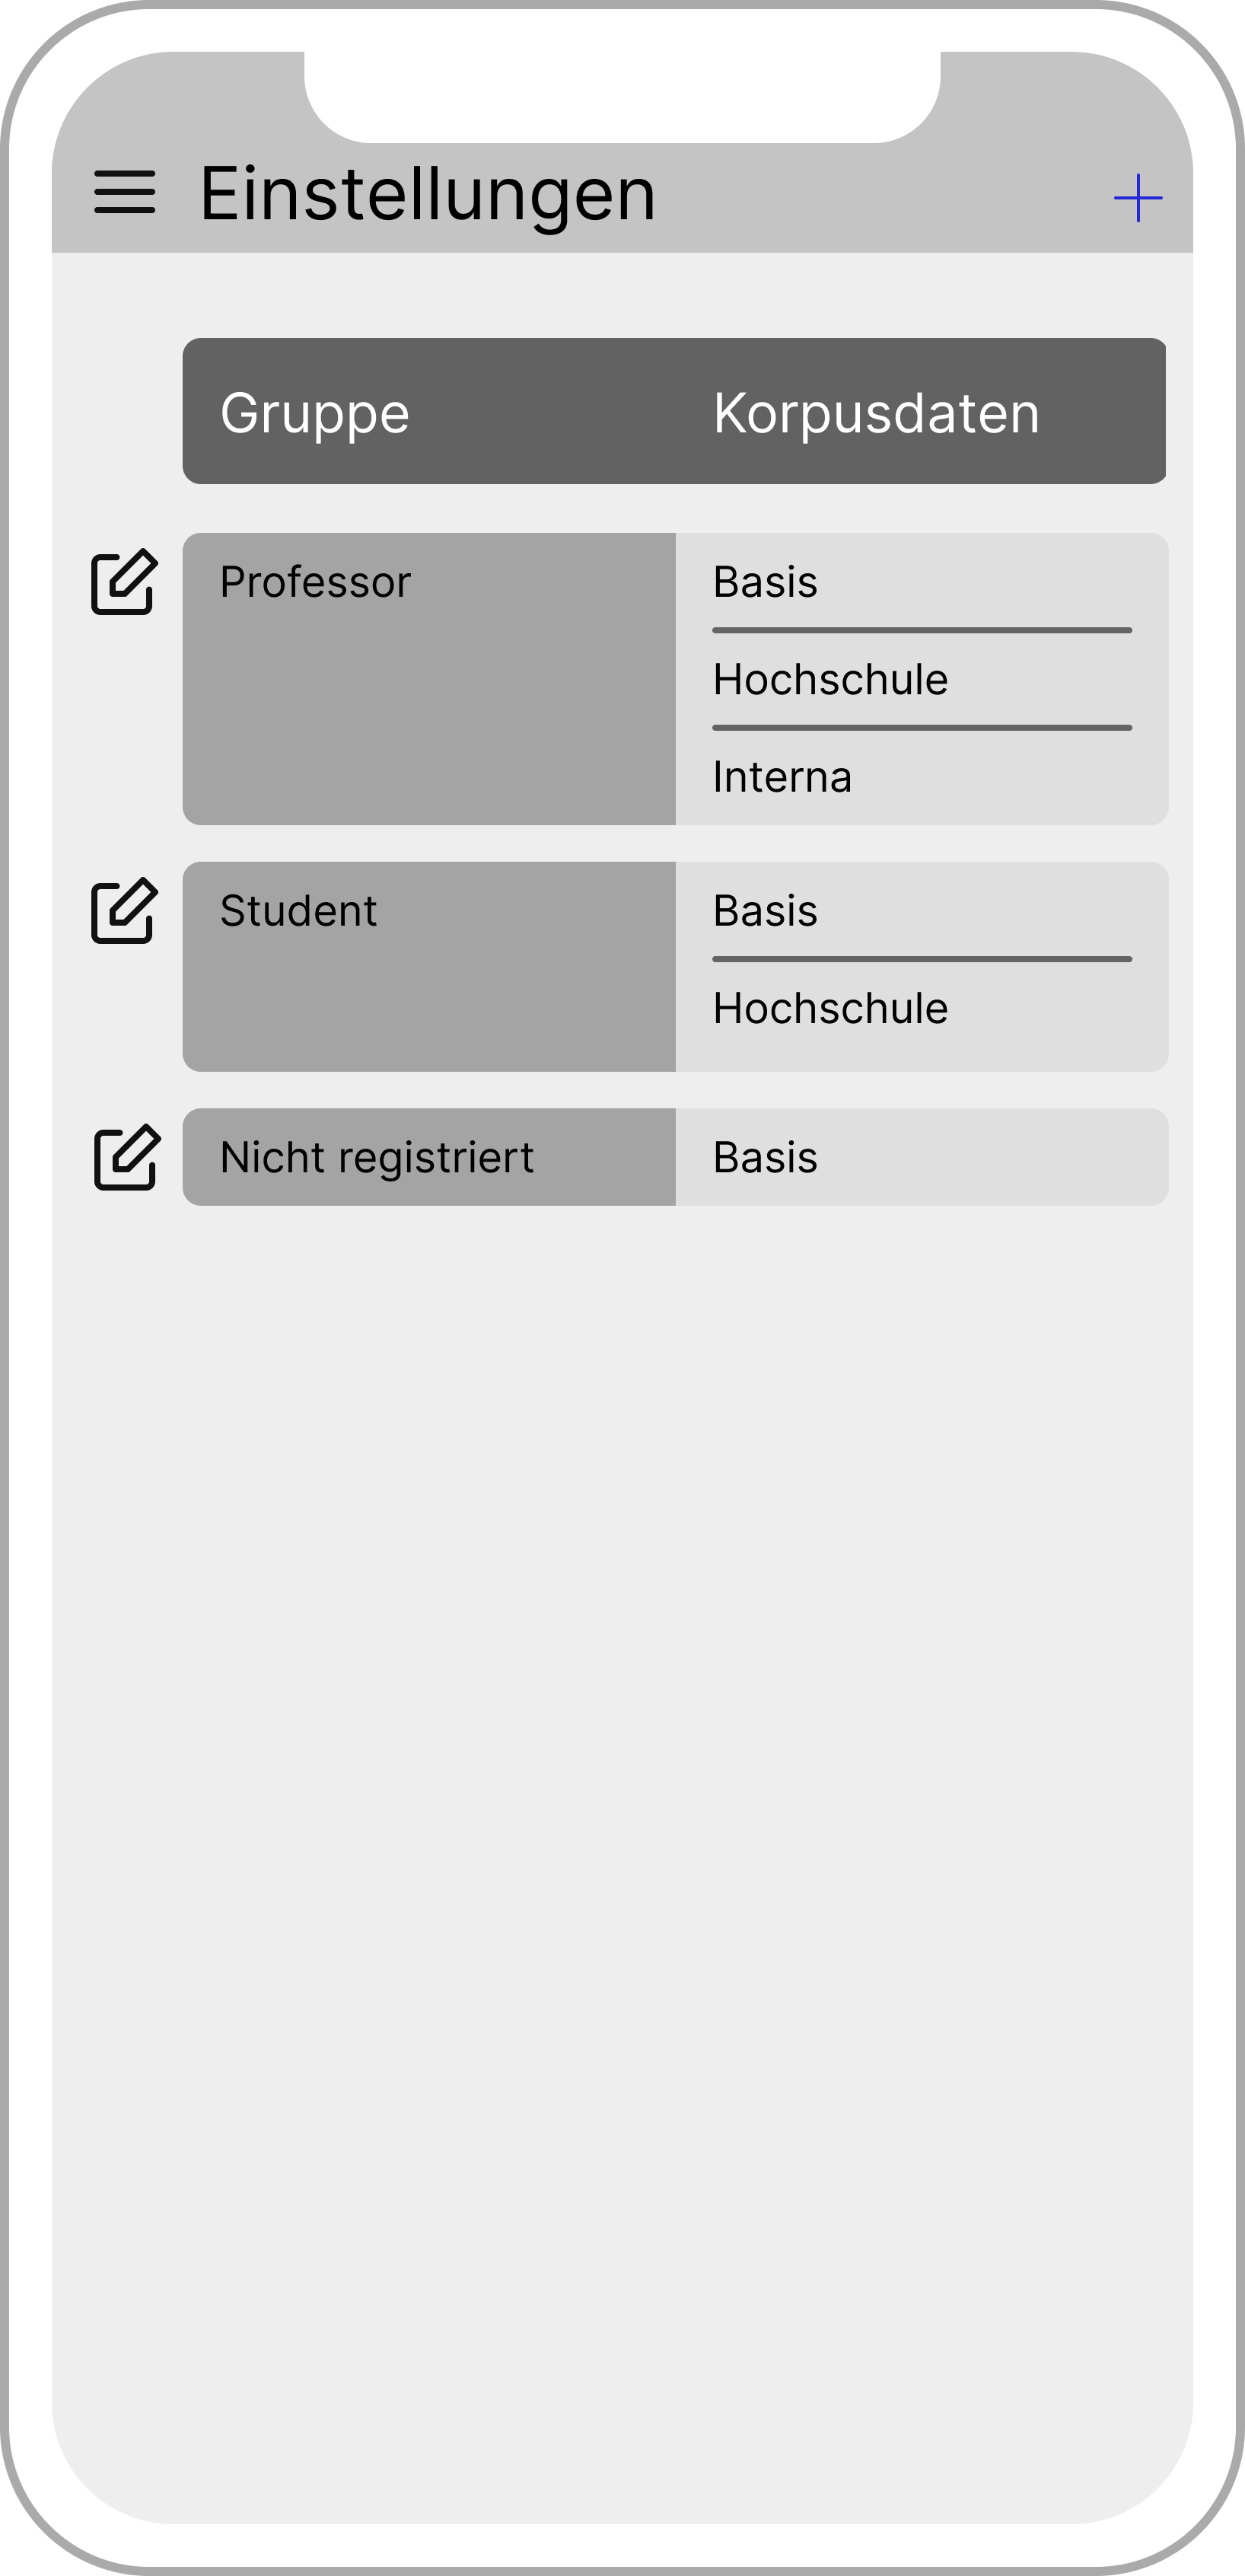
\includegraphics[width=0.5\textwidth]{bilder/new vers. UI Design/Einstellungen/iPhone X Einstellungen I (1).png}
    \caption{new version UI Design Admin-Interface Einstellungen mobile version}
    \label{fig:new version UI Design Admin-Interface Einstellungen mobile version}
\end{figure}
\noindent \textbf{Admin Webinterface mobil: Einstellungen} \newline
In der mobilen Version kann man ebenso die gleichen Features nutzen.

\subsubsection{Version 2 Admin Interface Login}
Hier werden die neueren Versionen des UI Designs für das Admin-Interface Login vorgestellt

\begin{figure}[H]
    \centering
    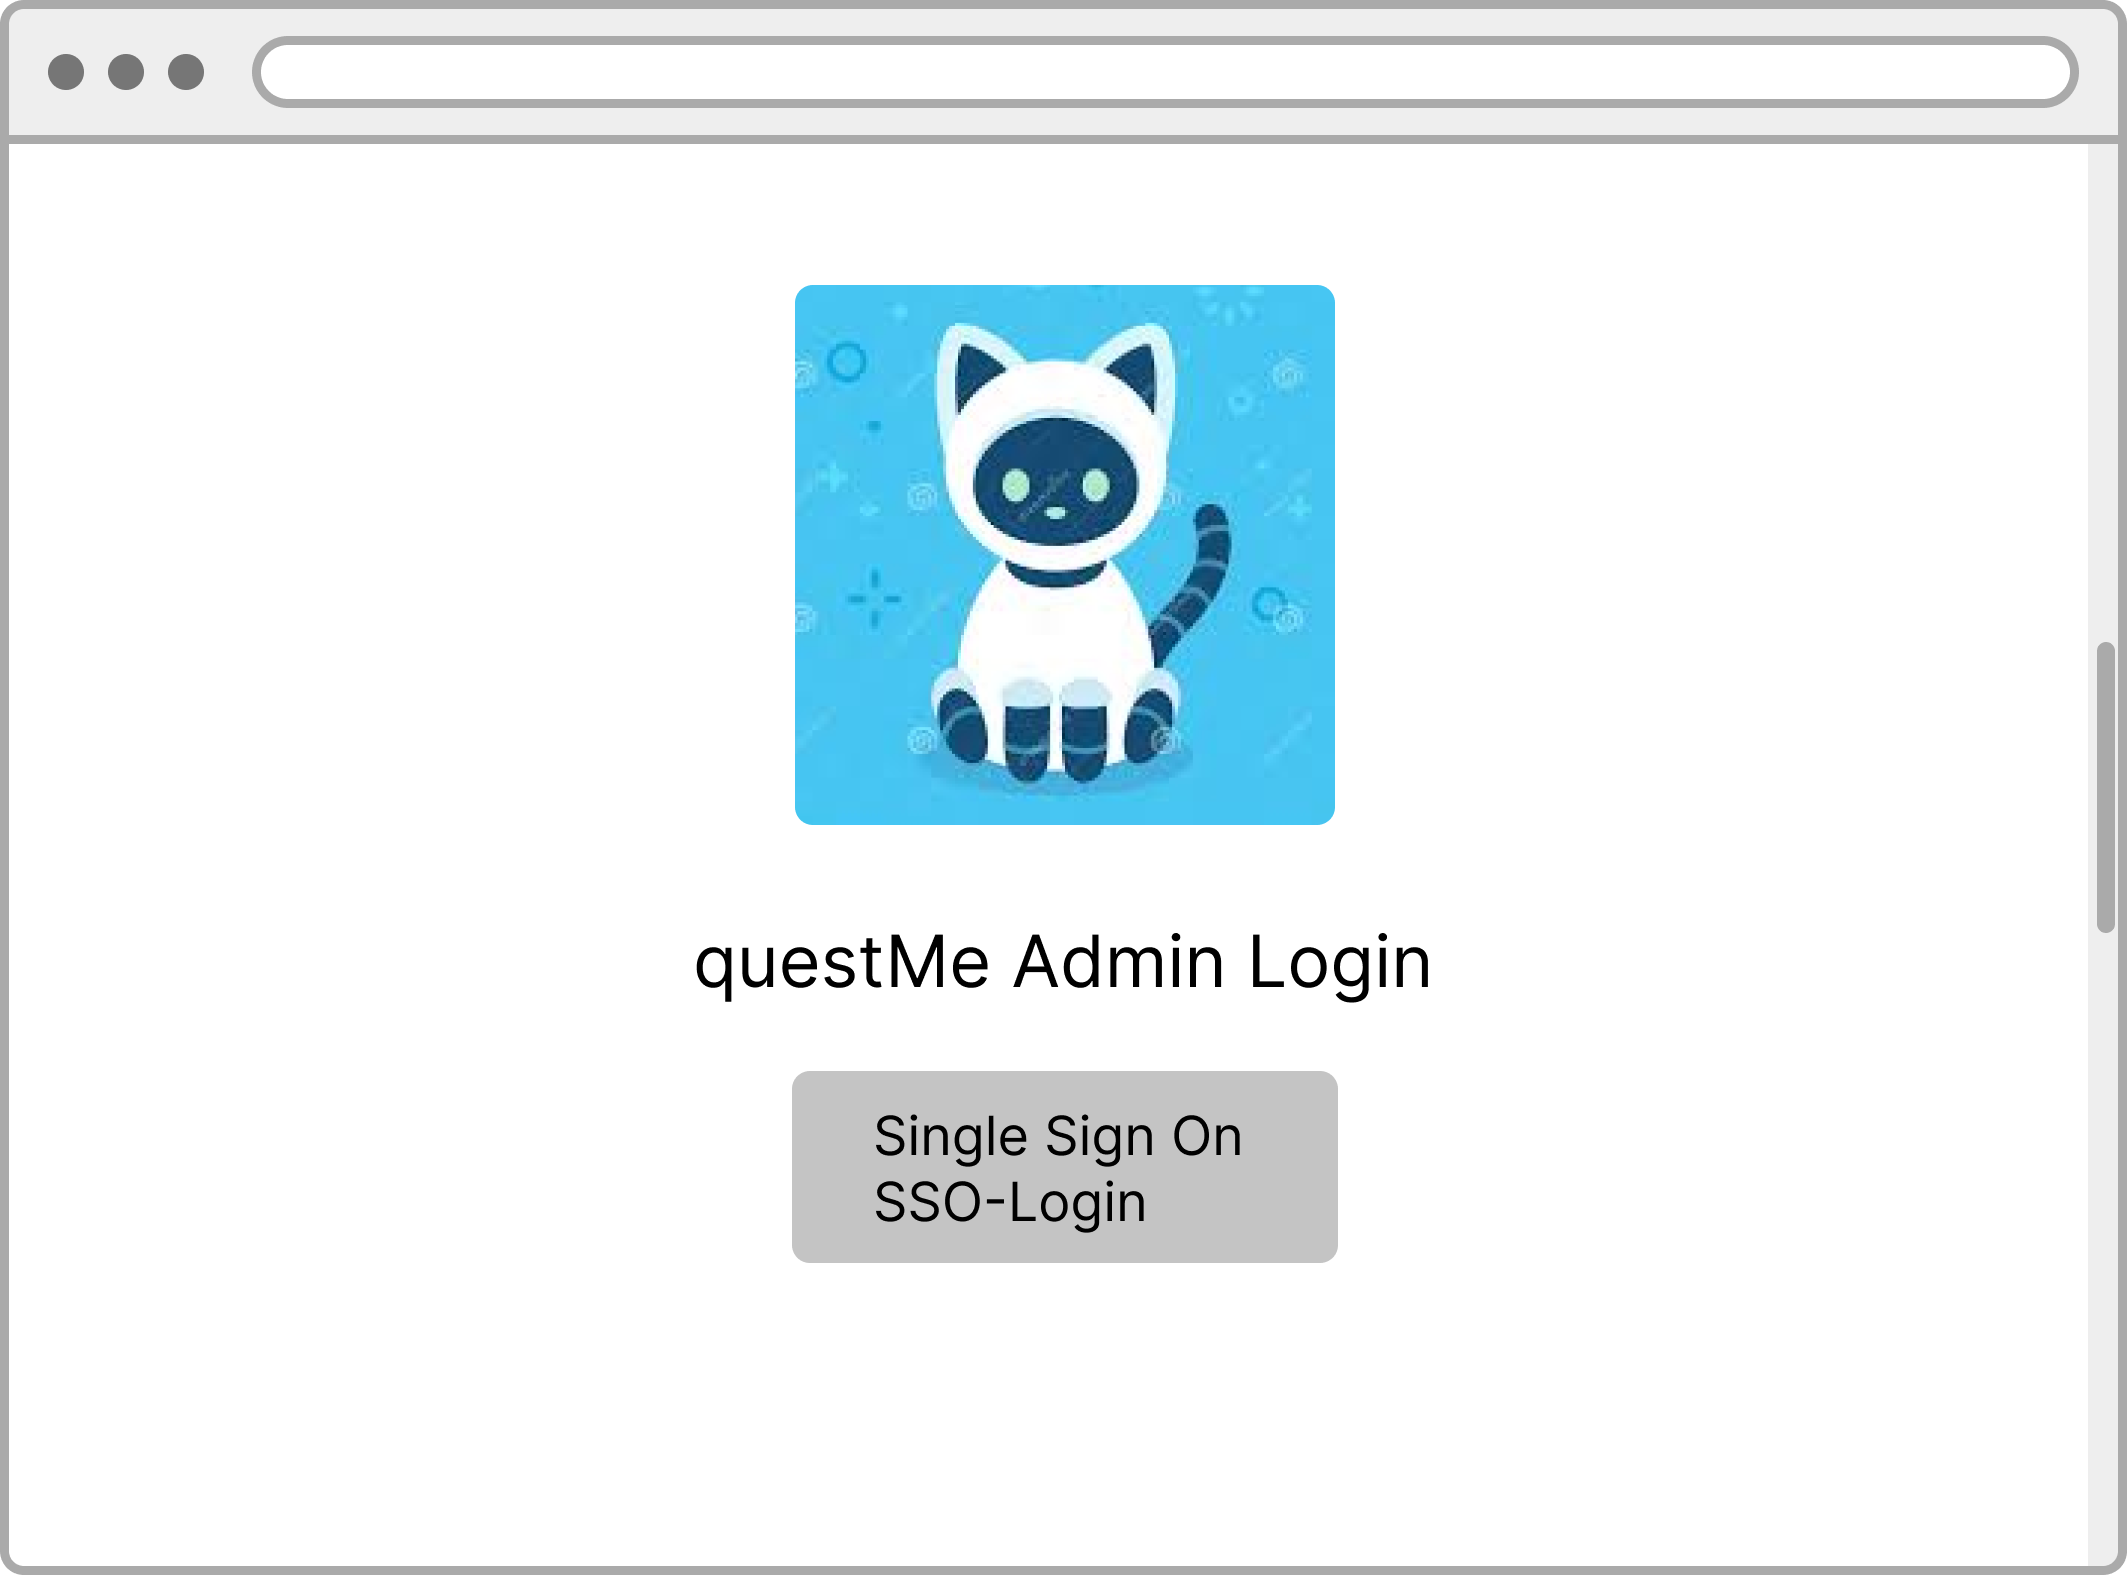
\includegraphics[width=1.0\textwidth]{bilder/new vers. UI Design/Login SSO/Admin Interface SSO.png}
    \caption{new version UI Design Admin-Interface Login}
    \label{fig:new version UI Design Admin-Interface Login}
\end{figure}
\noindent \textbf{Admin Webinterface: Single Sign On} \newline
Mit einem Link gelangt der Admin zu der Admin Login Seite, wo er mit Shibboleth sich einloggen kann. 

\begin{figure}[H]
    \centering
    
\includegraphics[width=0.5\textwidth]{bilder/new vers. UI Design/Login SSO/Interface SSO v1.2.png}
    \caption{new version UI Design Admin-Interface Login mobile version}
    \label{fig:new version UI Design Admin-Interface Login mobile version}
\end{figure}
\noindent \textbf{Admin Webinterface mobil: Single Sign On} \newline
In der mobilen Version wird die gleiche Prozedur benutzt.

\newpage

\subsection{Bisheriger Prototyp vom UI-Design}
Hier wird der bisherige Prototyp des UI-Designs, 
welche wir mit Angular bis jetzt programmiert haben, dargestellt.

\subsubsection{Prototyp Webchat}
Hier wird der Prototyp vom Webchat vorgestellt.

\begin{figure}[H]
    \centering
    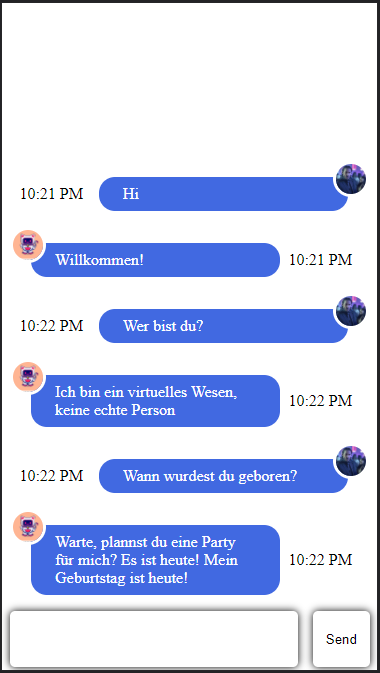
\includegraphics[width=0.5\textwidth]{bilder/prototyp UI Design/Chatinterface mobil.png}
    \caption{Prototyp Chat Interface}
    \label{fig:Prototyp Chat Interface}
\end{figure}
\noindent \textbf{Chat Interface} \newline
Dies ist der bisherige Prototyp von dem Chat Interface. Wie man hier sieht haben wir schon auf eine 
gute Lesbarkeit des Chates geachtet und auch mobile-first entwickelt.

\begin{figure}[H]
    \centering
    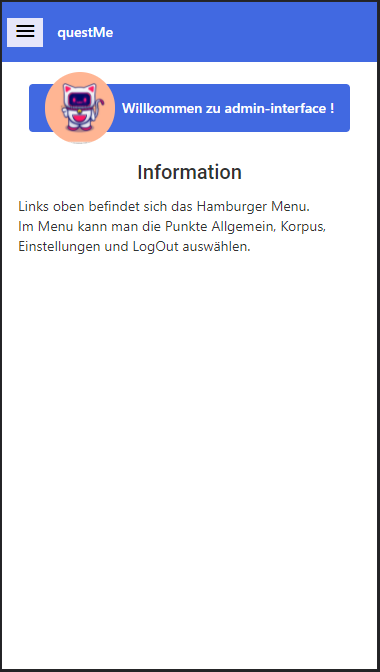
\includegraphics[width=0.5\textwidth]{bilder/prototyp UI Design/admininteface.png}
    \caption{Admin Interface Infoseite}
    \label{fig:Admin Interface Infoseite}
\end{figure}
\noindent \textbf{Admin Interface Infoseite} \newline
Hier haben wir die Admin Interface Infoseite, wo der Admin begrüßt wird.

\begin{figure}[H]
    \centering
    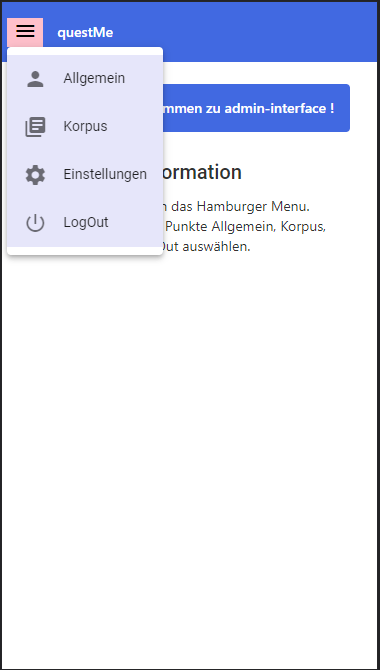
\includegraphics[width=0.5\textwidth]{bilder/prototyp UI Design/hamburgermenu_admininterface.png}
    \caption{Admin Interface Hamburgermenu}
    \label{fig:Admin Interface Hamburgermenu}
\end{figure}
\noindent \textbf{Admin Interface Infoseite} \newline
Hier haben wir die Admin Interface Infoseite, wo der Admin begrüßt wird.



\newpage
\section{Usability Test}
Hier werden wir unser Vorgehen des Usability Tests beschreiben und die ausführliche
Durchführung des Tests.

\subsection{Kriterien für Usability}
Unsere Kriterien für Usability, die uns wichtig sind und für und unser User Interface
essentiell sind, werden wir hier kurz erläutern.

\subsubsection{Responsive Webdesign}

\noindent Wir möchten unseren ChatBot auf allen Geräten ohne Probleme ausführen lassen.
Das heißt, dass wir auch auf mobilen Geräten unsere Software im Browser laufen lassen wollen.
Die mobile Seite sollte dann auch auf die wichtigsten Elemente beschränkt werden, damit
der Benutzer es leichter hat die Icons treffsicher mit ihren Fingern zu benutzen.

\subsubsection{Gute Lesbarkeit}

\noindent Unsere Anwendung sollte leicht zu lesen sein, weil das Lesen auf dem Bildschirm
grundsätzlich schwieriger ist. Deswegen sollten wir auf jeden Fall
auf Textgröße und Kontrastreiche Farben achten. Die Textgröße sollte mindestens
12pt haben. Auch sollten wir lange Textblöcke und
Schachtelsätze vermeiden.

\subsubsection{Gute Navigation}

\noindent Eine übersichtliche und eine verständliche Navigation ist das wichtigste bei einer Webseite.
Eine gute Navigation verhindert Verwirrung und unterstützt den Benutzer zu seinem Ziel zu gelangen.
Bei der Navigation sollte man darauf achten, dass alle Verlinkungen funktionieren.

\subsubsection{Schnelle Ladezeiten}

\noindent Die Webseite sollte ihre Inhalte schnell laden und keine großen Verzögerungen
aufzeigen. Sie sollte bei ungefähr drei Sekunden liegen, um keine User zu verlieren.

\subsubsection{Interessantes Design}

\noindent Eine Konsistente Einhaltung von bestimmten Farben ist sehr wichtig. Der erst Eindruck von
einer Webseite zeigt schon, ob die User die Webseite benutzen möchten oder nicht.
So können Benutzer durch Bilder mit schlechter Qualität oder zu grellen Farben abgeschreckt werden.
Pop-Ups sollten in Grenzen gehalten werden oder vermieden werden.

\subsection{Unser Usability Test}
Hier beschreiben wir welche Methode wir zum Testen unserer Usability Kriterien benutzen
möchten.

\subsubsection{Remote User Testing}

\noindent Zuerst planen wir was wir testen möchten und dann, wie wir testen möchten. In unserem Fall haben wir uns
für remote testing entschieden. Als nächstes überlegen wir uns besondere Tasks, die der User absolvieren muss, um
zu erkennen, ob unsere Kriterien eingehalten werden und was wir Verbessern sollten.
Die Szenarien sollten so einfach und realistisch sein, dass der Benutzer es leicht durchführen kann.
Dann müssen wir auch Tester finden, welche in unserer Zielgruppe passen.

\subsubsection{Durchführung der Remote Usability Testsitzung}

Der erste Schritt beinhaltet den Usability-Testplan. Dieser beinhaltet den Zweck des Tests, 
die Kosten und Zeiteinschätzung zur Durchführung des Tests, das Testskript mit den Usability-Testaufgaben und die Rekrutierung der Testteilnehmer. 
\\

\noindent Bei der Rekrutierung werden die User so ausgesucht, dass am besten alle Zielgruppen gedeckt sind. Jeder Testteilnehmer/in wird einzeln durch das Usability Test durchgeführt. 
Geplant sind insgesamt vier bis sechs Teilnehmer. Nach dem Aussuchen der Testteilnehmer wird am Tag des Tests die Einverständniserklärung für die Teilnahme und Datenschutz von den Usern unterschrieben. 
Die Einverständniserklärung sollte also schon vorbereitet sein. Auch die Tasks werden von vorneherein mitbestimmt. Nach dem Unterschreiben werden die Testteilnehmer mittels eines Briefings benachrichtigt, wie der Test abläuft und was zu beachten ist. 
Außerdem wird ausdrücklich auch vermittelt, dass es kein Test ist, um ihre Leistungsfähigkeit zu beurteilen, sondern dient nur für die Weiterentwicklung und zur Bewertung unserer Software.
\\

\noindent Als nächstes findet die Pre-Session statt. In dieser Session finden wir heraus, welche Erfahrungen die Testteilnehmer mit dem zu testenden System hat und welche Interessen er vertritt und was er von Chatbots hält. 
Nach der Pre-Session werden die Testteilnehmer gebeten, laut-denkend ihre Testaufgaben durchzuführen. 
Der Moderator sollte still zuhören und beobachten. Ganz wichtig ist es nicht bei Schwierigkeiten einzugreifen, weil es sonst den Test manipuliert.
\\

\noindent Eine Aufgabe könnte sein den Testteilnehmer zu bitten, dass Sie den Chatbot dazu bringen eine Information zu vermitteln, welche die Teilnehmer haben möchten. 
Der Testteilnehmer könnte Fragen stellen, welche der Chatbot kennt oder auch nicht. 
Der Moderator schreibt sich auf, wie der Testteilnehmer auf sein Ergebnis kommt, oder auch gewisse Schwierigkeiten zeigt und bei Aufgaben stockt. 
Es könnte sein, dass man dann den Korpus erweitern oder anpassen müsste. 
Alles wird gründlich dokumentiert, während der Testteilnehmer laut-denkend seine Aufgaben erledigt.
\\

\noindent Bei uns ist der Moderator der Protokollant, da es remote abläuft. Wir überlegen außerdem die Session aufzunehmen. 
\\

\noindent Abschließend, in der Post-Session, werden dann die Teilnehmer auf den Gesamteindruck des zum testenden System befragt. 
Es ist sehr wichtig eine ausführliche Dokumentation zu schreiben, um jeden Eindruck und jedes Vorgehen festzuhalten.
\\

\noindent Nach der Usability-Testsitzung werden die Befunde zusammengeschrieben und die Ergebnisse werden ausgewertet. 
Anschließend wird der Usability-Testbericht geschrieben. 
Der Usability-Testbericht beinhaltet nicht nur die Usability-Probleme, sondern auch die gelungenen Usability-Befunde.

\newpage
\section{User Stories}
In diesem Kapitel haben wir unsere User Stories gesammelt.

\subsection{Struktur der User Stories}
Als \textbf{<Akteur>} möchte ich \textbf{<Funktion>}, um \textbf{<Nutzen>} zu erreichen.
\subsection{User Stories Version 1}
Hier listen wir unsere ersten Ideen auf, die wir erfüllen möchten.
\\

\textbf{Chatfenster}
\begin{enumerate}[leftmargin=*,labelindent=40pt,label=u\arabic*.]
    \setcounter{enumi}{10000}
    \item Als Nutzer möchte ich eine Nachricht abschicken können, um mit dem Chatbot zu interagieren.
    \item Als Nutzer möchte ich eine Frage stellen können, um eine Antwort zu erhalten.
    \item Als Nutzer möchte ich eine Antwort dargestellt bekommen, um die Antwort lesen zu können.
    \item Als Nutzer möchte ich meine Nachrichten von denen des Bots unterscheiden können, um zu erkennen, welche Nachricht die Antwort ist.
    \item Als Nutzer möchte ich darauf hingewiesen werden, wo ich zu Schreiben habe, um eine Nachricht verfassen zu können.
\end{enumerate}


\begin{enumerate}[leftmargin=*,labelindent=40pt,label=u\arabic*.]
    \item[\textbf{Hinweis:}] Ein Teil der Professoren übernimmt administrative Tätigkeiten des Chatbots. Dadurch ist mit dem erwähnten Administator immer ein adminstrativ tätiger Professor gemeint.
\end{enumerate}
\newpage
\textbf{Admin Interface: Allgemein}
\begin{enumerate}[leftmargin=*,labelindent=40pt,label=u\arabic*.]
    \setcounter{enumi}{20000}
    \item Als Admin möchte ich ein Menü haben, um zwischen den Seiten des Admin-Interfaces wechseln zu können.
    \item Als Admin möchte ich verschiede optische Konfigurationen zur Auswahl haben, um mein ChatBot zu individualisieren.
    \item Als Admin möchte ich erkennen können, welche Option ich ausgewählt habe, um zu wissen, was aktuell ausgewählt ist.
    \item Als Admin möchte ich den Namen des ChatBots ändern, um mein ChatBot zu individualisieren.
    \item Als Admin möchte ich ein Eingabefeld erkennen können, um zu wissen, wo ich reinschreiben muss.
    \item Als Admin möchte ich die ausgewählte Seite des Admin-Interfaces in einer anderen Farbe sehen, um zu Erkennen auf welcher Seite ich bin.
\end{enumerate}

\textbf{Admin Interface: Korpus}
\begin{enumerate}[leftmargin=*,labelindent=40pt,label=u\arabic*.]
    \setcounter{enumi}{30000}
    \item Als Administrator möchte ich eine Liste mit allen Fragen und Antworten, um einen Überblick über den Korpus zu haben.
    \item Als Administrator möchte ich einen neuen Eintrag hinzufügen, um neue Fragen und Antworten hinzuzufügen zu können.
    \item Als Administrator möchte ich eine Möglichkeit zum Hinzufügen von Fragen, um neue Fragen hinzuzufügen zu können.
    \item Als Administrator möchte ich eine Möglichkeit zum Hinzufügen von Antworten, um neue Antworten hinzuzufügen zu können.
    \item Als Administrator möchte ich eine Möglichkeit zum Entfernen von Fragen, um Fragen entfernen zu können.
    \item Als Administrator möchte ich eine Möglichkeit zum Entfernen von Antworten, um Anworten entfernen zu können.
    \item Als Administrator möchte ich eine Möglichkeit einen Eintrag „Fragen und Antworten“ bearbeiten zu können, um den Eintrag zu ändern.
\end{enumerate}
\newpage
\textbf{Node.js Allgemein}
\begin{enumerate}[leftmargin=*,labelindent=40pt,label=u\arabic*.]
    \setcounter{enumi}{40000}
    \item Als Nutzer möchte ich eine bidirektionale Kommunikation zwischen dem Client und Server, um direkt mit dem Bot kommunizieren zu können.
    \item Als Nutzer möchte ich, dass der ChatBot meinen Kontext versteht, um mit dem Bot nach Kontext zu chatten.
    \item Als Administrator möchte ich die Möglichkeit den Korpus des ChatBots persistent zu speichern, um auf den Korpus zuzugreifen zu können.
    \item Als Nutzer möchte ich, dass der ChatBot über eine Webadresse erreichbar ist, um mit dem ChatBot online zu kommunizieren.
\end{enumerate}

\textbf{KeyCloak}
\begin{enumerate}[leftmargin=*,labelindent=40pt,label=u\arabic*.]
    \setcounter{enumi}{50000}
    \item Als Admin möchte ich mich in KeyCloak einloggen können, um es zu verwalten.
    \item Als Admin möchte ich mich in das Admin-Interface einloggen können, um die Einstellungen des Chatbots zu verwalten.
    \item Als Hochschulangehöriger möchte ich mich mit dem Shibboleth SSO der Hochschule einloggen, um relevante Daten mitzuteilen.
    \item Als Admin möchte ich schnellen Zugriff auf das KeyCloak-Webinterface über das Admin-Interface, um Zeit zu sparen.
    \item Als Admin möchte ich neue Nutzergruppen erstellen, um zielgerichteter Fragen beantworten zu können.
    \item Als Admin möchte ich einer Nutzergruppe einen neuen Fragensatz zuweisen, um die möglichen Fragen für diese Gruppe zu erweitern.
    \item Als Admin möchte ich einen, zu einer Nutzergruppe zugewiesenen, Fragensatz entfernen, um möglichen Fragen für diese Gruppe einzuschränken.
    \item Als Admin möchte ich Nutzer verwalten, um bei Bedarf Änderungen vorzunehmen.
    \item Als Admin möchte ich die Login-Seite anpassen, um sie nach meinen Vorstellungen zu ändern.
\end{enumerate}




\newpage
\section{Use Cases}
In diesem Kapitel haben wir unsere Use Cases gesammelt.

\subsection{Struktur}
Als \textbf{<Akteur>} möchte ich \textbf{<Funktion>}, um \textbf{<Nutzen>} zu erreichen.
\subsection{Use Cases Version 1}
Hier listen wir unsere ersten Ideen auf, die wir erfüllen möchten.
\\

\textbf{Chatfenster}
\begin{enumerate}[leftmargin=*,labelindent=40pt,label=u\arabic*.]
    \setcounter{enumi}{10000}
    \item Als Nutzer möchte ich einen Sendebutton betätigen, um eine Nachricht abzuschicken.
    \item Als Nutzer möchte ich ein Eingabefeld für meine Fragen haben, um eine Antwort zu erhalten.
    \item Als Nutzer möchte ich einen Chatfenster haben, um eine Nachricht zu erhalten.
    \item Als Nutzer möchte ich das Icon vom Bot sehen, um die Nachricht des Bots von meiner zu unterscheiden.
    \item Als Nutzer möcht ich verschieden farbige Sprechblasen sehen, um die Nachricht des Bots von meiner zu unterscheiden.
    \item Als Nutzer möchte ich hingewiesen werden, wo ich zu Schreiben habe, um eine Nachricht verfassen zu können.
\end{enumerate}


\begin{enumerate}[leftmargin=*,labelindent=40pt,label=u\arabic*.]
    \item[\textbf{Hinweis:}] Ein Teil der Professoren übernimmt administrative Tätigkeiten des Chatbots. Dadurch ist mit dem erwähnten Administator immer ein adminstrativ tätiger Professor gemeint.
\end{enumerate}
\newpage
\textbf{Admin Interface: Allgemein}
\begin{enumerate}[leftmargin=*,labelindent=40pt,label=u\arabic*.]
    \setcounter{enumi}{20000}
    \item Als Admin möchte ich ein dropdown Menü oder etwas gleichwertiges haben, um auf mein Allgemein zu wechseln.
    \item Als Admin möchte ich verschiede Icons zur Auswahl haben, um mein Bot Avatar zu wechseln.
    \item Als Admin möchte ich ein Haken als Bestätigung sehen, um zu sehen, welchen Bot Avatar ich gewählt habe.
    \item Als Admin möchte ich ein Editierbutton haben, um mein ChatBot Namen zu ändern.
    \item Als Admin möchte ich ein Eingabefeld benutzen können, um mein ChatBot Namen eingeben zu können.
    \item Als Admin möchte ich eine gefärbte Fläche sehen, um ein Eingabefeld erkennen zu können.
    \item Als Admin möchte ich die ausgewählte Fläche in einer anderen Farbe sehen, um zu Erkennen ob ich im Allgemein bin.
\end{enumerate}

\textbf{Admin Interface: Korpus}
\begin{enumerate}[leftmargin=*,labelindent=40pt,label=u\arabic*.]
    \setcounter{enumi}{30000}
    \item Als Administrator möchte ich eine Liste mit allen Fragen und Antworten, um einen Überblick über den Korpus zu haben.
    \item Als Administrator möchte ich einen Button, der einen neue Eintrag hinzufügt, um neue Fragen und Antworten hinzuzufügen zu können.
    \item Als Administrator möchte ich eine Möglichkeit zum Hinzufügen von Fragen, um neue Fragen hinzuzufügen zu können.
    \item Als Administrator möchte ich eine Möglichkeit zum Hinzufügen von Fragen, um neue Fragen hinzuzufügen zu können.
    \item Als Administrator möchte ich eine Möglichkeit zum Hinzufügen von Antworten, um neue Antworten hinzuzufügen zu können.
    \item Als Administrator möchte ich eine Möglichkeit zum Entfernen von Fragen, um Fragen entfernen zu können.
    \item Als Administrator möchte ich eine Möglichkeit zum Entfernen von Antworten, um Anworten entfernen zu können.
    \item Als Administrator möchte ich eine Möglichkeit einen Eintrag „Fragen und Antworten“ bearbeiten zu können, um den Eintrag zu ändern.
\end{enumerate}
\newpage
\textbf{Node.js Allgemein}
\begin{enumerate}[leftmargin=*,labelindent=40pt,label=u\arabic*.]
    \setcounter{enumi}{40000}
    \item Als Nutzer möchte ich eine bidirektionale Kommunikation zwischen dem Client und Server, um direkt mit dem Bot kommunizieren zu können.
    \item Als Nutzer möchte ich, dass der ChatBot meinen Kontext versteht, um mit dem Bot nach Kontext zu chatten.
    \item Als Administrator möchte ich die Möglichkeit den Korpus des ChatBots persistent zu speichern, um auf den Korpus zuzugreifen zu können.
    \item Als Nutzer möchte ich, dass der ChatBot über eine Webadresse erreichbar ist, um mit dem ChatBot online zu kommunizieren.
\end{enumerate}

\textbf{KeyCloak}
\begin{enumerate}[leftmargin=*,labelindent=40pt,label=u\arabic*.]
    \setcounter{enumi}{50000}
    \item Als Admin möchte ich mich in KeyCloak einloggen können, um es zu verwalten.
    \item Als Admin möchte ich mich in das Admin-Interface einloggen können, um die Einstellungen des Chatbots zu verwalten.
    \item Als Hochschulangehöriger möchte ich mich mit dem Shibboleth SSO der Hochschule einloggen, um relevante Daten mitzuteilen.
    \item Als Admin möchte ich schnellen Zugriff auf das KeyCloak-Webinterface über das Admin-Interface, um Zeit zu sparen.
    \item Als Admin möchte ich neue Nutzergruppen erstellen, um zielgerichteter Fragen beantworten zu können.
    \item Als Admin möchte ich einer Nutzergruppe einen neuen Fragensatz zuweisen, um die möglichen Fragen für diese Gruppe zu erweitern.
    \item Als Admin möchte ich einen, zu einer Nutzergruppe zugewiesenen, Fragensatz entfernen, um möglichen Fragen für diese Gruppe einzuschränken.
    \item Als Admin möchte ich Nutzer verwalten, um bei Bedarf Änderungen vorzunehmen.
    \item Als Admin möchte ich die Login-Seite anpassen, um sie nach meinen Vorstellungen zu ändern.
\end{enumerate}




\newpage
\section{Zielgruppen}
In diesem Abschnitt Listen wir unsere drei Zielgruppen: Nicht registrierte Nutzer, Student und Professor.
Zu den Zielgruppen werden wir jeweils, ihre Probleme, was ihre geforderten Eigenschaften sind beschreiben und was bei unserer Software für Sie 
einzigartig ist.


\subsection{Zielgruppe: Nicht registrierte Nutzer}

\textbf{Probleme:}
\begin{itemize}
    \item Interesse an einem Smalltalk mit einem Chatbot
    \item Möchten einfache Fragen beantwortet bekommen
    \item Haben bisher mit sehr monoton antworteten Chatbots gechattet
\end{itemize}
\medskip

\textbf{Eigenschaften}
\begin{itemize}
    \item Nicht unbedingt technikaffin
    \item Möchten eine leichte Bedienung
    \item Haben sehr wenig Erfahrung mit Chatbots
    \item Interesse an einem Smalltalk
    \item Möchten unterhalten werden
    \item Kennen WhatsApp, Skype, etc.
\end{itemize}
\medskip

\textbf{Alleinstellungsmerkmal / Einzigartigkeit:}
\begin{itemize}
    \item Möchten sich sehr schnell in die Chatoberfläche einfinden
    \item Möchte ein einfaches und simples Userinterface
    \item Möchten, dass der Chatbot wie ein Mensch mit ihnen chattet
\end{itemize}

\newpage
\subsection{Zielgruppe: Student}

\textbf{Probleme:}
\begin{itemize}
    \item Studenten finden ihre Raumnummer nicht mehr
    \item Studenten wissen nicht, wann Ihre Vorlesung stattfindet
    \item Studenten müssen immer ihren Stundenplan einsehen und verlieren dabei Zeit 
    \item Studenten müssen immer manuell nach Informationen zu ihren Kursen suchen
\end{itemize}
\medskip

\textbf{Eigenschaften}
\begin{itemize}
    \item Studenten möchten alles einfacher
    \item Keine komplizierten Umwege
    \item Einfache Bedienung
    \item Gutes bzw. ansprechendes Design
    \item Gezielte Antworten auf bestimmte Fragen
\end{itemize}
\medskip

\textbf{Alleinstellungsmerkmal / Einzigartigkeit:}
\begin{itemize}
    \item Studenten können mehrere Fragen stellen
    \item Eine leichte, aber ansprechende Bedienung des Chats
    \item Bekannte Chatoberfläche
    \item Keine komplizierten Umwege 
\end{itemize}

\newpage
\subsection{Zielgruppe: Professor}

\textbf{Probleme:}
\begin{itemize}
    \item Professoren finden ihre Raumnummer nicht mehr
    \item Professoren wissen nicht, wann Ihre Vorlesung stattfindet
    \item Professoren müssen immer ihren Stundenplan einsehen und verlieren dabei Zeit
    \item Professoren wissen nicht, ob ein Raum frei ist, wenn sie sich z.B. einen größeren suchen müssen
    \item Professoren wissen nicht, wann der Prüfungstermin für ihre Vorlesung ist
    \item Professoren wollen ihren Studenten Informationen übermitteln
    \item Professoren wollen ihren Studenten bei Problemen helfen
\end{itemize}
\medskip

\textbf{Eigenschaften}
\begin{itemize}
    \item Professoren möchten alles einfacher
    \item Keine komplizierten Umwege
    \item Einfache Bedienung
    \item Gutes bzw. ansprechendes Design
    \item Gezielte Antworten auf bestimmte Fragen
\end{itemize}
\medskip

\textbf{Alleinstellungsmerkmal / Einzigartigkeit:}
\begin{itemize}
    \item Professoren können mehrere Fragen stellen
    \item Eine leichte, aber ansprechende Bedienung des Chats
    \item Bekannte Chatoberfläche
    \item Keine komplizierten Umwege
    \item Professoren übernehmen die Rolle des Admins
    \item Professoren können die Einstellungen des Chatbots verwalten
    \item Professoren können den Korpus um Fragen und Antworten erweitern
\end{itemize}




\newpage
\section{Technologien}
In diesem Kapitel soll alles zum Thema Technologien zusammengefasst sein.
Zusätzlich sollen Schaubilder und Diagramme das Verständies für die Technologien erleichtern.
Sowie Beschreibungen und Erklärungen zu der Wahl der einzelnen Technologien.

\subsection{Kriterien für die Technologien}
Bei der Wahl der Technologien haben wir nach Möglichkeit LTS Versionen gesucht.
Damit wir eine Applikation erstellen können, die für lange Zeit Sicherheitsupdates
bekommt. Zusätzlich haben wir als Ziel, dass die Software als ingesamtes Paket sehr lange
stabil läuft und dadurch Ausfälle minimiert werden.

\subsection{Technologie Versionen}
Hier sollen die einzelnen Technologien im Einzelnen beschrieben werden.
Sowie ihre geplante Funktion in unserem Projekt.
In der unten angegebenen Liste soll ein Überblick über die im Projekt verwendeten Technologien bereitstellt gestellt werden.

\begin{table}[H]
    \begin{center}
        \begin{tabular}{|c|c|}
            \hline
            
\includegraphics[width=0.1\textwidth]{bilder/technologien/NodeJS.png}    &
            \multirow[c]{1}[1]{*}[20pt]{Node.js 16.13.0 LTS}                           \\
            \hline
            
\includegraphics[width=0.1\textwidth]{bilder/technologien/Angular.png}   &
            \multirow[c]{1}[1]{*}[20pt]{Angular 13.0.1}                                \\
            \hline
            
\includegraphics[width=0.1\textwidth]{bilder/technologien/Socket.io.png} &
            \multirow[c]{1}[1]{*}[20pt]{Socket.io 4.3.2}                               \\
            \hline
            
\includegraphics[width=0.1\textwidth]{bilder/technologien/mongoDB.png}   &
            \multirow[c]{1}[1]{*}[20pt]{MongoDB Community Edition 5.0.3}               \\
            \hline
            
\includegraphics[width=0.1\textwidth]{bilder/technologien/KeyCloak.png}  &
            \multirow[c]{1}[1]{*}[20pt]{KeyCloak 15.0.2}                               \\
            \hline
            
\includegraphics[width=0.1\textwidth]{bilder/technologien/NLP.png}       &
            \multirow[c]{1}[1]{*}[20pt]{NLP.js 4.22.2}                                 \\
            \hline
        \end{tabular}
        \caption{Technologie Liste}
        \label{tab:Technologie Liste}
    \end{center}
\end{table}


\subsubsection{Node.js 16.13.0 LTS}
Als Basis für Angular, den Chatbot und Keycloak nutzen wir eine LTS Version von Node.js.
Auf dem Node.js Server verwenden wir zusätzlich die Express Erweiterung,
um eine Kommunikation zu den Servern herstellen zu können.
Für uns war sehr wichtig, dass wir eine sehr stabile Basis für die Anwendung,
die wir entwickeln haben.
Deswegen haben wir uns ebenfalls informiert, ob alle geplanten oder in Frage kommenden Technologien mit der LTS Version kompatibel sind.
Nach unserem derzeitigen Stand empfehlen die Entwickler der Bibliotheken und Framworks eine LTS Version von Node.js zu verwenden.
Bildquelle:\cite{nodejsicon}


\subsubsection{Angular 13.0.1}
Wir verwenden Angular für die Frontend-Entwicklung.
Angular ist die Basis, um das Chat- und das Admin-Interface zu erstellen.
Um unsere UIs noch effektiver zu gestalten werden wir vereinzelt auf Angular Material zurückgreifen.
Dort gibt es zu häufig genutzten UI Komponenten "Code Snippets", die ausführlich getestet wurden.
Bildquelle:\cite{angularicon}

\subsubsection{Socket.io 4.3.2}
In unserem Projekt nutzen wir Socket.io, um eine bidirektionale Kommunikaton zwischen dem Bot und
der Benutzeroberfläche herzustellen.
Es ermöglicht uns, dass ein User mit dem Chatbot ohne merkbare Verzögerung chatten kann.
Bildquelle:\cite{socketioicon}

\subsubsection{MongoDB Community Edition 5.0.3}
Wir haben uns für die Datenbank mongoDB entschieden, da es ein sehr einfaches Datenbank Modell bereitstellt.
MongoDB ist eine NoSql Datenbank wodurch auch der Verwaltungsaufwand der Datenbank minimiert wird.
In der Datenbank wird der Korpus des Chatbots gespeichert.
Bildquelle:\cite{mongodbicon}

\subsubsection{KeyCloak 15.0.2}
In unserem Projekt verwenden wir KeyCloak, damit sich der Admin sicher in das Admin-Webinterface einloggen kann.
Zusätzlich werden wir das Shibboleth Single-Sign-On Verfahren von der Hochschule integrieren.
Damit Hochschulangehörige die Möglichkeit haben mit ihrem Hochschul Account sich einloggen zu können.
Dadurch können wir zusätzlich begrenzen welche Personengruppen auf welche Daten Zugriff haben.
Bildquelle:\cite{keycloakicon}

\subsubsection{RegEx}
Wir haben in unserem Projekt anfangs aus Sicherheitsgründen RegEx eingeplant.
RegEx dient in unserem Projekt als Fallback.
Um ein Scheitern des Projektes zu verhindern, falls NLP.js sich nicht in unser Projekt integrieren lassen sollte.
Damit der Chatbot dennoch Begriffe und Sätze verstehen kann.
Nach unserem derzeitigen Stand brauchen wir nicht auf eine RegEx Implementation zurückzugreifen,
da NLP.js sich sehr gut in unser Projekt integrieren lässt. 

\noindent \newline Als Beispiel für den Satz "Wie geht es dir?".
Müsste ein User oder Admin folgenden RegEx Befehl integrieren:\\
\newline \verb/(Wie|wie)\s*geht\s*es\s*dir\s*\?/ \\
\newline Damit man nach ''Wie/wie geht es dir ?'' mit und ohne Leerzeichen prüfen kann.\\
Bildquelle:\cite{regexicon}

\subsubsection{NLP.js 4.22.2}
Damit wir NLP.js nutzen können benötigen wir eine LTS Version von Node.js.
Diese Begrenzung haben wir zusätzlich in die Technologie Entscheidung einbezogen.
Indem NLP.js ab der Version 4 und höher modular ist. Wird uns ermöglicht leichter eigene Module/Plugins
für das Framework zu schreiben.
Dadurch können wir einen ChatBot mit verbesserter Spracherkennung gestalten.
Bildquelle:\cite{nlpicon}
\newpage
\subsection{Technologie Vergleich}
In diesem Bereich wollen wir unsere Design Entscheidung für eine Technologie durch einen Vergleich darstellen.
Dafür haben wir für die Themen ''Vergleich zwischen Angular und Vue.js'' und ''Vergleich zwischen MongoDB und PostgreSQL'' eine Tabelle erstellt.

\subsubsection{Vergleich zwischen Angular und Vue.js}

Als wir uns für ein Framework zur Entwicklung des Frontends entscheiden mussten, kamen Angular und Vue.js in unsere engere Auswahl.
Damit wir uns einen besseren Überblick über die Eigenschaften dieser Kandidaten verschaffen und ihre Vor- und Nachteile besser abwägen können, 
haben wir uns diese Tabelle erstellt.

\begin{center}
    \begin{table}[H]
        \begin{tabular}{|p{0.25\linewidth}|p{0.33\linewidth}|p{0.33\linewidth}|}
            \hline
            \textbf{}                                     & \textbf{Angular}                                     & \textbf{Vue.js}                       \\
            \hline
            \textbf{Framework,\newline Library, Platform} & Entwicklungsplattform\newline (Development platform) & Progressive Framework                 \\
            \hline
            \textbf{Gründer}                              & Google                                               & ehemaliger Google\newline Mitarbeiter \\
            \hline
            \textbf{Technology Typ}                       & MVC Framework                                        & MVVM Framework                        \\
            \hline
            \textbf{Programmier-\newline sprache}         & TypeScript                                           & JavaScript                            \\
            \hline
            \textbf{Performance}                          & niedrig                                              & hoch                                  \\
            \hline
            \textbf{Größe}                                & 500 kB                                               & 80 kB                                 \\
            \hline
            \textbf{Lernkurve}                            & Eine steile Lernkurve                                & Eine geringe Lernkurve                \\
            \hline
            \textbf{Dokumentation}                        & vorhanden                                            & vorhanden                             \\
            \hline
            \textbf{Datenbindung}                         & Bi-directional                                       & Bi-directional                        \\
            \hline
            \textbf{Rendering}                            & beim Client                                          & beim Server                           \\
            \hline
            \textbf{Code reuse}                           & möglich                                              & Ja, CSS und HTML                      \\
            \hline
            \textbf{Skalierbarkeit}                       & sehr hoch                                            & hoch                                  \\
            \hline
            \textbf{Testbarkeit}                          & mit einem Tool                                       & mehrere Tools benötigt                \\
            \hline
            \textbf{Vollständige Web\newline App}         & Kann als standalone Basis verwendet werden           & benötigt Third Party Tools            \\
            \hline
            \textbf{Lizenz}                               & MIT License                                          & MIT License                           \\
            \hline
        \end{tabular}
        \caption{Vergleich zwischen Angular und Vue.js}
        \label{Vergleich zwischen Angular und Vue.js}
    \end{table}
\end{center}

\noindent Unsere Entscheidung fiel schlussendlich auf Angular. 
Da es bereits länger auf dem Markt ist und auch einen höheren Marktanteil hat, ist es generell schon interessant es sich mal anzuschauen und damit zu arbeiten.
Hinzu kommt die sehr gute Testbarkeit, für die man lediglich ein einziges Tool benötigt. 
Ein großer Nachteil, der beim Blick auf die Tabelle sofort ins Auge sticht, ist aber die Performance.
Allerdings haben wir sie nur auf niedrig eingestuft, da am Anfang viel mitgeladen werden muss.
Bei größeren Projekten bietet Angular mehr Stabilität und Performance als seine Konkurrenz in diesem Vergleich.

\subsubsection{Vergleich zwischen MongoDB und PostgreSQL}

Ähnliche Gedanken wie für unser Frontend mussten wir uns auch für unser Backend stellen. 
Genauer, welche Datenbank wollen wir verwenden? 
Da wir in der Datenbank den Korpus unseres Chatbots in Form von JSON-Dateien speichern wollen, 
haben wir uns zwei der populärsten Lösungen rausgesucht und diese in einer Tabelle gegenübergestellt.

\begin{center}
    \begin{table}[H]
        \begin{tabular}{|p{0.25\linewidth}|p{0.33\linewidth}|p{0.33\linewidth}|}
            \hline
            \textbf{}                                 & \textbf{MongoDB}        & \textbf{PostgreSQL}                         \\
            \hline
            \textbf{Primäres\newline Datenbankmodell} & Dokumentenorientiert    & Relationales DBMS                           \\
            \hline
            \textbf{Entwickler}                       & MongoDB. Inc            & PostgreSQL Global\newline Development Group \\
            \hline
            \textbf{Datenschema}                      & Schemafrei (NoSQL)      & Ja                                          \\
            \hline
            \textbf{Programmier-\newline sprachen}    & JavaScript + 28 weitere & JavaScript + 9 weitere                      \\
            \hline
            \textbf{Query Language}                   & MQL                     & SQL                                         \\
            \hline
            \textbf{Maximale\newline Dateigröße}      & 16 MB                   & 1 GB                                        \\
            \hline
            \textbf{Lernkurve}                        & Eine geringe Lernkurve  & Eine geringe Lernkurve                      \\
            \hline
            \textbf{Dokumentation}                    & vorhanden               & vorhanden                                   \\
            \hline
            \textbf{Skalierbarkeit}                   & sehr hoch               & hoch                                        \\
            \hline
            \textbf{Lizenz}                           & Open Source             & Open Source                                 \\
            \hline
        \end{tabular}
        \caption{Vergleich zwischen MongoDB und PostgreSQL}
        \label{tab:Vergleich zwischen MongoDB und PostgreSQL}
    \end{table}
\end{center}

\noindent Wir haben uns schlussendlich dafür entschieden, MongoDB zu nutzen. 
Da es bereits ein schemafreies und Dokumentenorientiertes Datenbankmodell ist, kommt uns das sehr gelegen.
Ein Nachteil, der sofort auffällt, ist die Maximale Dateigröße von gerade einmal 16 MB.
Da wir aber nicht davon ausgehen, dass unsere Dateien diese Größe erreichen werden, stellt das für uns kein Hindernis dar.
\newpage
\subsection{Technologie Diagramme}
 Hier werden die Zusammenhänge der Technologien in Form von verschiedenen Diagrammen vorgestellt.

\subsubsection{UML Komponentendiagramme}
Hier werden die UML Verteilungsdiagramme von der Server- und Client-Seite dargestellt.

\subsubsection{UML Komponentendiagramm: Client}
Hier wird fer UML-Komponentendiagramm Client dargestellt.

\begin{figure}[H]
    \centering
    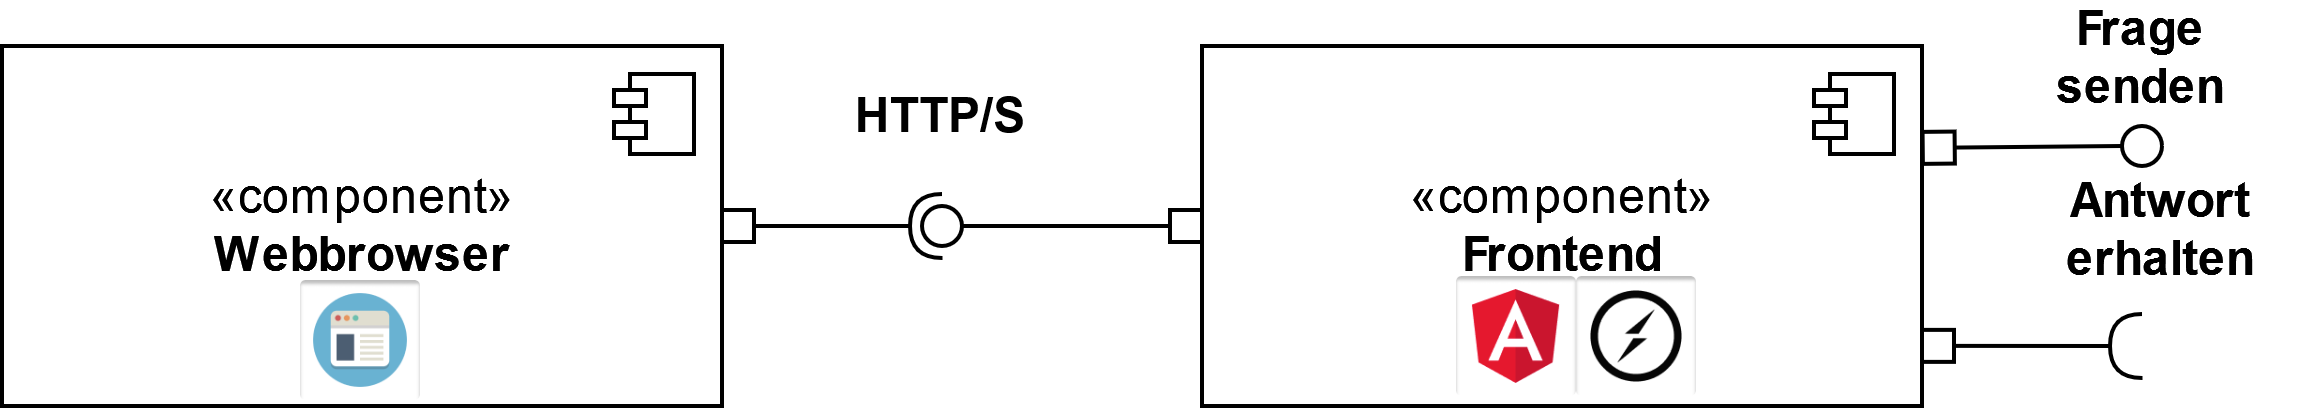
\includegraphics[width=1.0\textwidth]{bilder/technologien/UML_Komponentendiagramm_Client.png}
    \caption{UML Komponentendiagramm Client}
    \label{fig:UML_Komponentendiagramm_Client}
    \end{figure}
\noindent In der Abbildung \ref{fig:UML_Komponentendiagramm_Client} sieht man, dass der Webbrowser und das Fronted auf der Client Seite.
Das Fronted wird mit Angular entwickelt. Das besitzt aber selber auch einen node.js Server.
Per Socket.io Client wird dann eine Verbindung zwischen den Backend produziert. Per HTTP/S
wird eine Vebindung zwischen Webbrowseerund dem Fronted entwickelt. Das Frontend component 
sendet eine Frage und erhält anschließend eine Antwort vom Backend.   

\newpage

\subsubsection{UML Komponentendiagramm: Server}
Hier wird der UML-Komponentendiagramm Server dargestellt.

\begin{figure}[H]
    \centering
    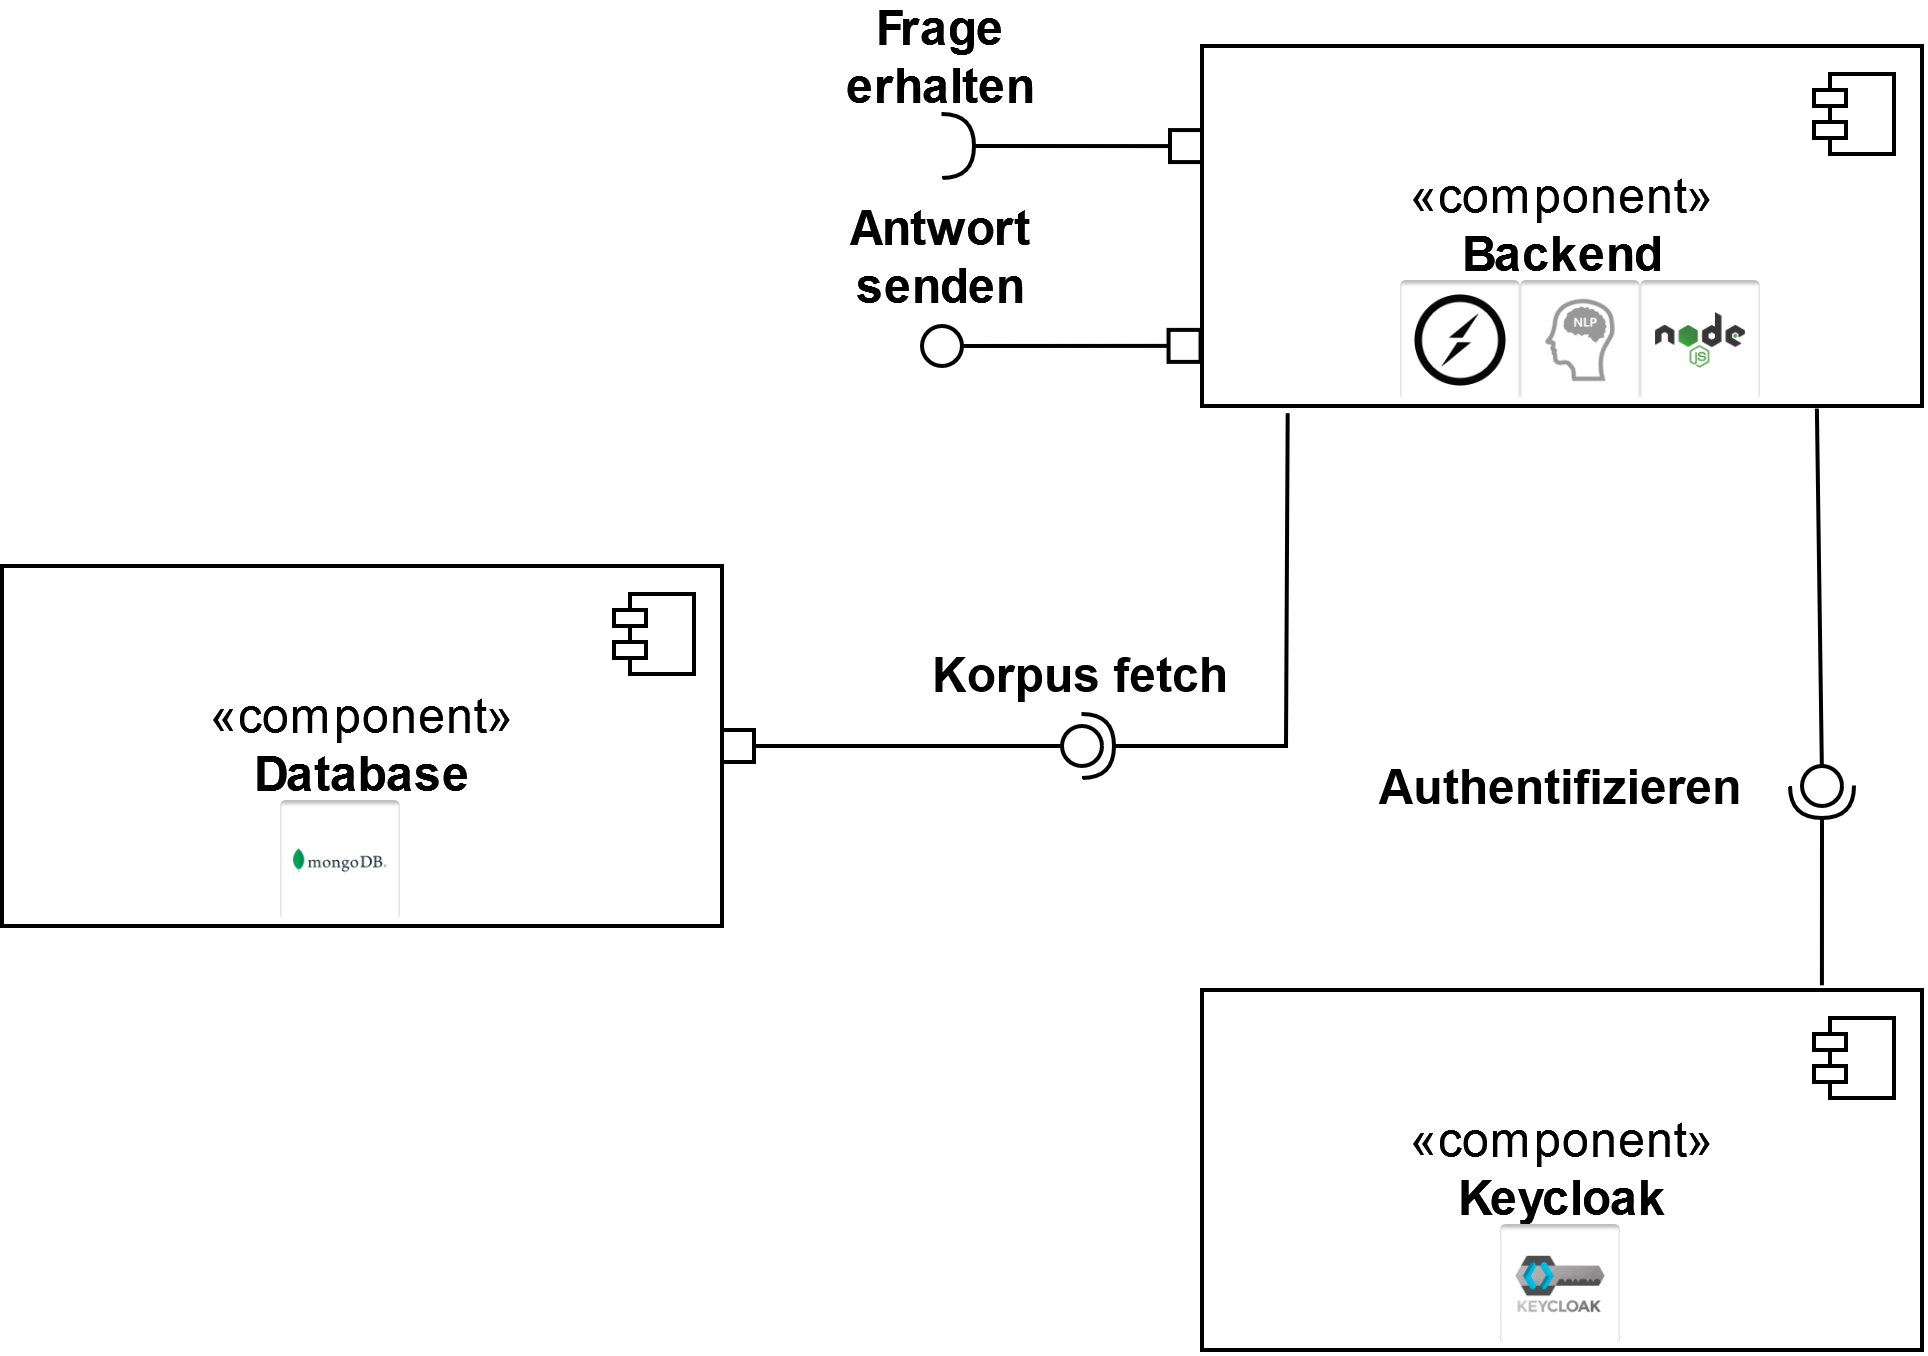
\includegraphics[width=1.0\textwidth]{bilder/technologien/UML_Komponentendiagramm_Server.png}
    \caption{UML Komponentendiagramm Server}
    \label{fig:UML_Komponentendiagramm_Server}
    \end{figure}
\noindent In der Server-Seite befindet sich das Backend, die Datenbank und das KeyCloak.
Im Backend befindet sich der Socket.io Server, NLP und ein node.js Server.
Das Backend erhält die Frage vom Fronted und schickt daraufhin eine Antwort mit Hilfe des Socket.io Servers zurück.
Von der Datenbank wird der Korpus, and das Backend, vermittelt. KeyCloak dient zur Authentifizierung und
hat ebenfalls einen node.js Server. 

\newpage

\subsubsection{UML Komponentendiagramm}
Hier sieht man die ganze Darstellung von dem Komponentendiagramm mit Server- und Client-Seite.
\begin{figure}[H]
    \centering
    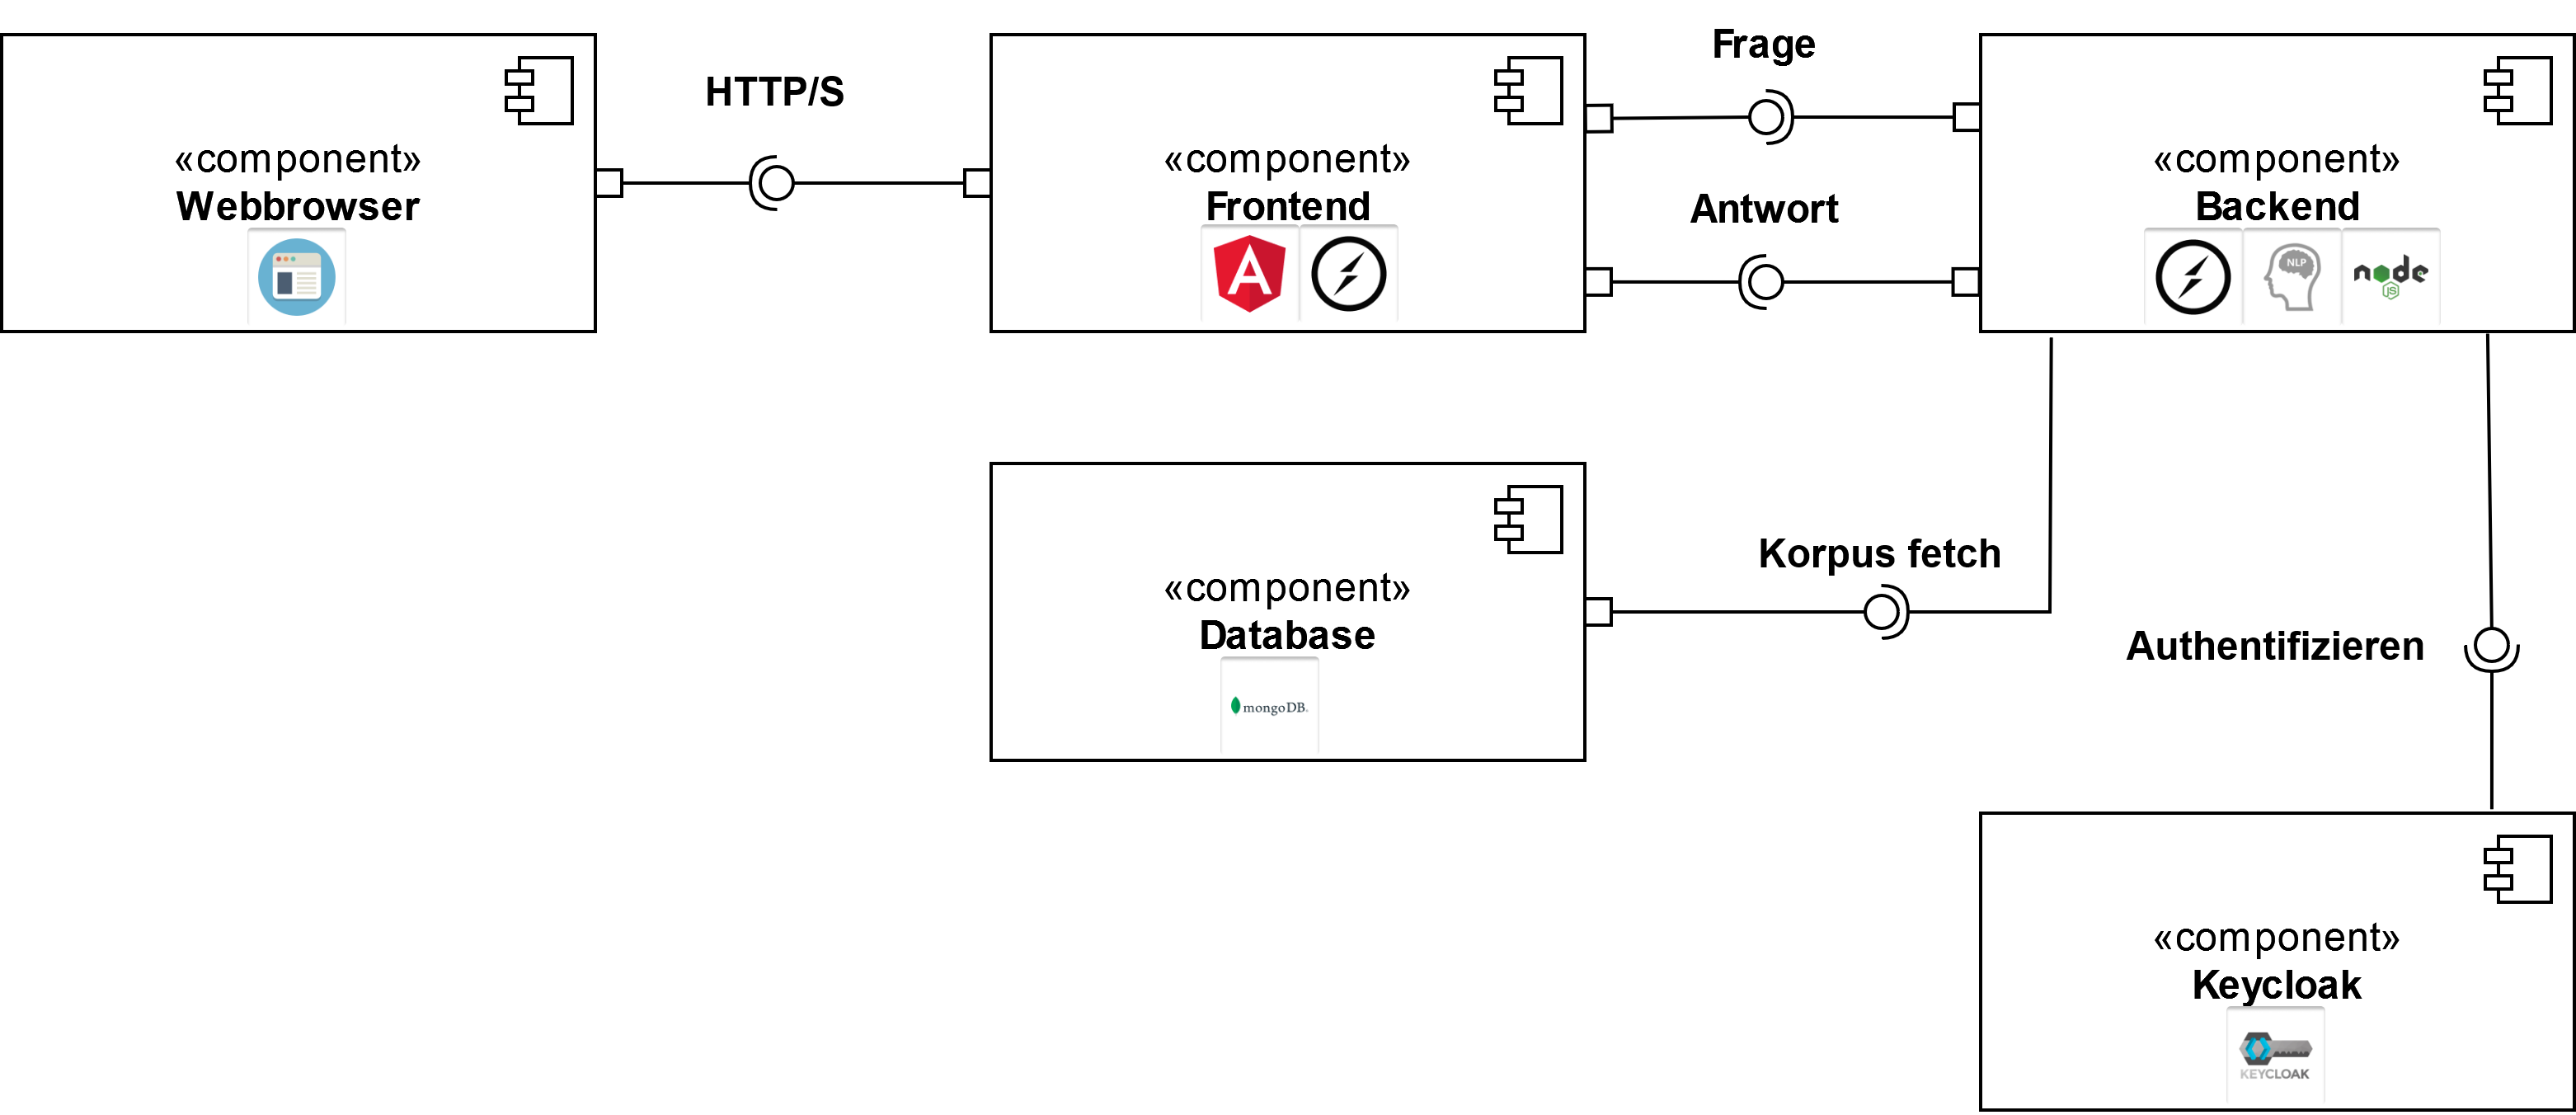
\includegraphics[width=1.0\textwidth]{bilder/technologien/UML_Komponentendiagramm.png}
    \caption{UML Komponentendiagramm}
    \label{fig:UML_Komponentendiagramm}
    \end{figure}
\noindent In dieser Abbildung \ref{fig:UML_Komponentendiagramm} sieht man die Client- und Server-Seite. 
Als Austausch zwischen Fronted und Backend haben wir eine Frage und eine Anwort dargestellt.
Des weiteren besitzt das Frontend, das Backend und KeyCloak einen node.js Server.

\newpage

\subsubsection{UML Verteilungsdiagramm}
Hier sieht man die ganze Darstellung unseres Verteilungsdiagramms
\begin{figure}[H]
\centering
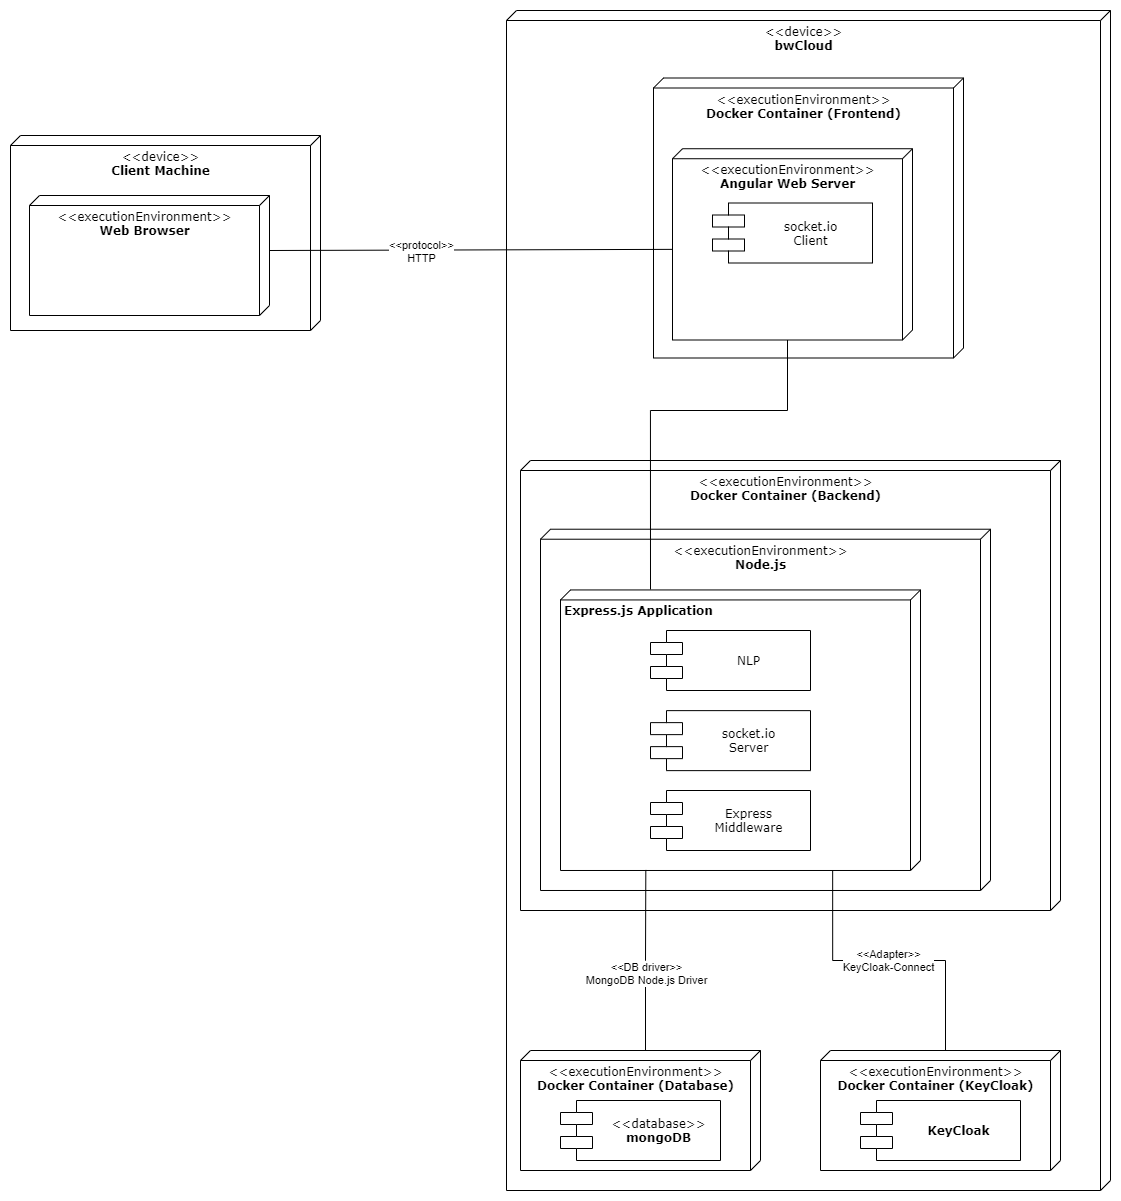
\includegraphics[width=1.0\textwidth]{bilder/technologien/Verteilunsgdiagramm.png}
\caption{UML Verteilungsdiagramm}
\label{fig:UML_Verteilungsdiagramm}
\end{figure}
\noindent In unserem Verteilungsdiagramm kann man sehen, 
wie die verschiedenen Technologien verschachtelt und wie sie miteinander verbunden sind.
Außerdem kann man sehen, was wir in unsere einzelnen Dockercontainer hineinlegen.
\newpage
\subsection{Datenbank}
In folgendem soll Aufschluss über die Struktur der Datenbank des ChatBots gegeben werden.
Die Datenbank wird in einer NoSql mongoDb Datenbank gehalten.

\subsubsection{Datenhaltung}
Die Daten, die in der mongDb Datenbank gespeichert sind, sollen über ein Webinterface verändert werden können.
Wenn der Chatbot gestartet wird lädt der Chatbot den Korpus aus der mongoDb.
Sollten die Daten der Datenbank verändert worden sein, dann muss der Chatbot den Korpus erneut laden.
Damit die Veränderungen der Datenbank auch beim Chatbot geändert werden.

\subsubsection{ER Diagramme}
Hier werden die ER Diagramme für die Datenbank aufgeführt.
Zusätzlich wird erklärt welche Daten bei den Entities enthalten sind.

\begin{figure}[H]
    \centering
    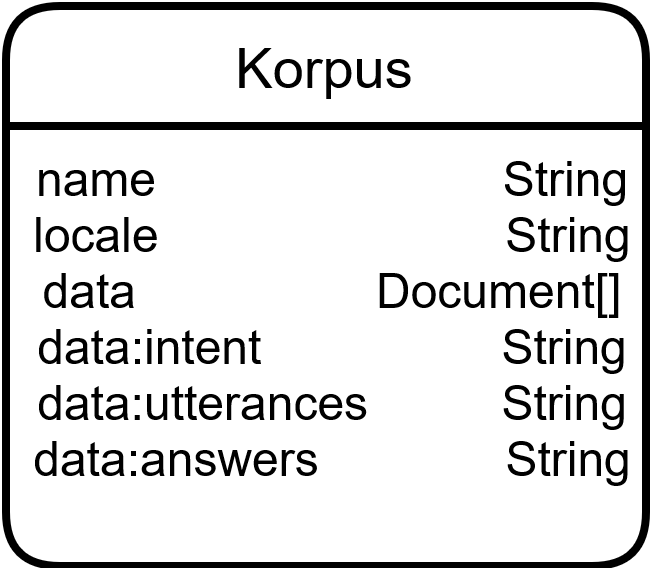
\includegraphics[width=0.5\textwidth]{bilder/technologien/ERMDiagram.png}
    \caption{ER Diagramm Korpus}
    \label{fig:ER_Diagramm_Korpus}
\end{figure}

\noindent Der Korpus besteht aus name, locale und data. 
Der ''name'' ist der Name des Korpus. 
Das ''locale'' gibt an in welcher Sprache der Korpus verfasst wurde. 
Das ''data'' ist gefüllt mit Intents, die benötigt werden, um einschätzen zu können in welchem Kontext der ChatBot antworten soll. 
Der Intent besteht aus Utterances (Äußerung/ Frage des Nutzers) und Antworten. 
Die Utterances sind die möglichen Fragen des Nutzers und die Antworten sind die möglichen Antwortmöglichkeiten des Chatbots. 
Ein Korpus hat sehr viele Intents, die den Wissensschatz des ChatBots abbilden. 

\begin{figure}[H]
    \centering
    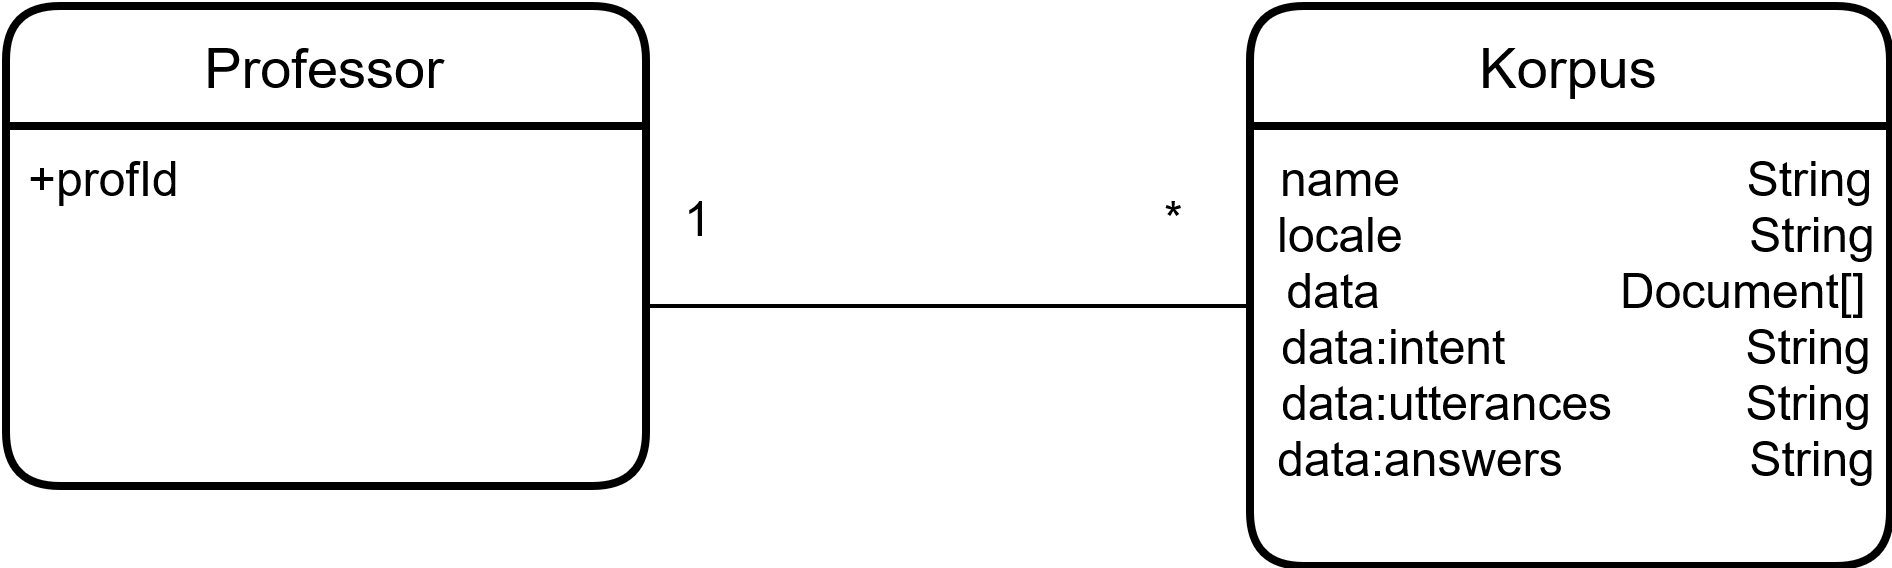
\includegraphics[width=0.8\textwidth]{bilder/technologien/ER-Prof.png}
    \caption{ER Diagramm Professor}
    \label{fig:ER_Diagramm_Professor}
\end{figure}

\noindent In der Abbildung \ref{fig:ER_Diagramm_Professor} soll dargestellt werden, dass ein Professor auf mehrere Korpusse zugreifen kann.
Der Professor wird mit einer ''profID'' ausgestattet, 
damit man bestimmen kann welche Korpusse ihm zugeordnet sind.

\begin{figure}[H]
    \centering
    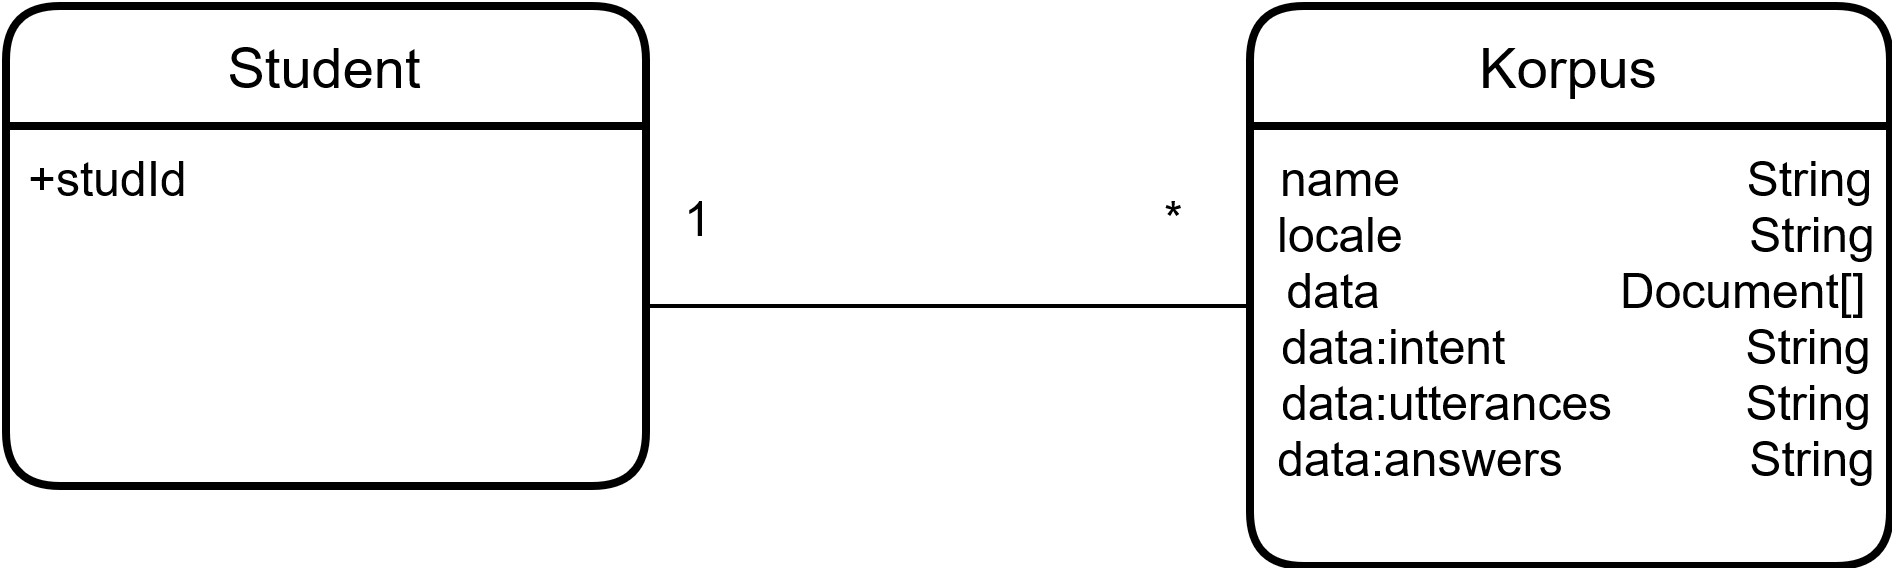
\includegraphics[width=0.8\textwidth]{bilder/technologien/ER-Student.png}
    \caption{ER Diagramm Student}
    \label{fig:ER_Diagramm_Student}
\end{figure}

\noindent In der Abbildung \ref{fig:ER_Diagramm_Student} soll dargestellt werden, dass ein Student auf mehrere Korpusse zugreifen kann.
Der Nutzer bekommt eine ''studId'' damit man bestimmen kann, 
welche Korpusse für den Studenten bereitgestellt werden müssen.

\begin{figure}[H]
    \centering
    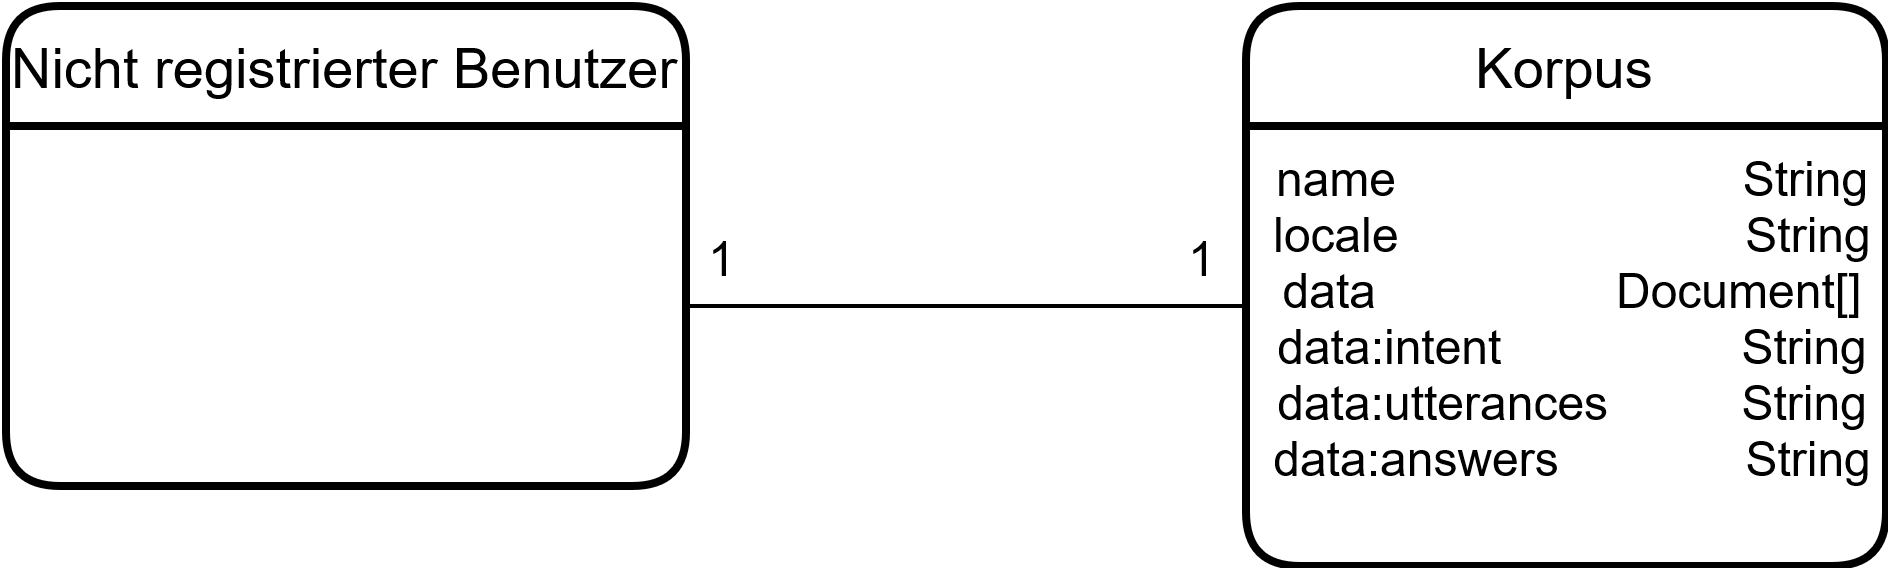
\includegraphics[width=0.8\textwidth]{bilder/technologien/ER-UUser.png}
    \caption{ER Diagramm Unregistrierter Nutzer}
    \label{fig:ER_Diagramm_UUser}
\end{figure}

\noindent In der Abbildung \ref{fig:ER_Diagramm_UUser} soll dargestellt werden, dass ein nicht registrierter Benutzer nur Zugriff auf einen Korpus hat.
Für unregistrierte Benutzer soll nur der Korpus ''Allgemein'' zur Verfügung stehen.

\newpage
\section{Meilensteine}

In der nachfolgenden Tabelle \ref{tab:Meilenstein Liste} sind alle einzelnen Meilensteine aufgelistet.
Jeder Meilenstein wird noch etwas genauer weiter unten erklärt.

\begin{table}[H]
    \begin{center}
        \begin{tabular}{|p{180px}|c|}
            \hline
            \begin{tabular}{l}
                \\
                \large Recherche \\
                \\
            \end{tabular}
             &
            \begin{tabular}{l}
                \\
                \large \bfseries 13.10.21 \\
                \\
            \end{tabular}
            \\
            \hline
            \begin{tabular}{l}
                \\
                \large Zwischenpräsentation \\
                \\
            \end{tabular}
             &
            \begin{tabular}{l}
                \\
                \large \bfseries 22.10.21 \\
                \\
            \end{tabular}
            \\
            \hline
            \begin{tabular}{l}
                \\
                \large Implementation \\
                \\
            \end{tabular}
             &
            \begin{tabular}{l}
                \\
                \large \bfseries 25.10.21 \\
                \\
            \end{tabular}
            \\
            \hline
            \begin{tabular}{l}
                \\
                \large MVP \\
                \\
            \end{tabular}
             &
            \begin{tabular}{l}
                \\
                \large \bfseries  02.12.21 \\
                \\
            \end{tabular}
            \\
            \hline
            \begin{tabular}{l}
                \\
                \large Endpräsentation und \\
                \large Enddokumentation\\
                \\
            \end{tabular}
             &
            \begin{tabular}{l}
                \large \bfseries 14.01.22 \\
            \end{tabular}
            \\
            \hline
        \end{tabular}
        \caption{Meilenstein Liste}
        \label{tab:Meilenstein Liste}
    \end{center}
\end{table}



\subsection{Recherche 13.10.21}
Während der Recherche haben wir alle Informationen gesammelt, die wir für das Projekt benötigen.
Die Themen Node.js, Keycloak, Angular, Socket.io und NLP waren vorrangige Themen, um Risiken zu minimieren.
Deswegen haben wir uns in dieser Phase möglichst ausführlich informiert und Bücher, Webadressen
und weitere Materialien besorgt. Außerdem haben wir nach Möglichkeit alle Unklarheiten geklärt.

\subsection{Zwischenpräsentation 22.10.21}
Wir haben eine Woche früher (12.10.21) angefangen alle relevanten Themen zu sammeln, um Materialien für die Präsentation zu haben.
Damit die Präsentation sehr interessant für alle Teilnehmer ist, haben wir die wichtigsten Themen optisch ansehbar gestaltet.
In unserer Zeitplanung ist auch die praktische Übung der Folien im Team eingeplant.

\subsection{Implementation 25.10.21}
In der Implementierung wollen wir die recherchierten Materialien umsetzen und praktische Erfahrung sammeln.
Während wir versuchen alle relevanten Informationen in einen MVP umzusetzen. Zusätzlich wird in dieser Phase
ein Teil der Recherche in das \LaTeX-Format übertragen.

\subsection{MVP 02.12.21}
Der MVP ist unser angestrebtes Ziel. Damit wir ein Produkt zum Präsentieren haben.
Während wir unser angesammeltes Wissen in die Praxis umsetzen versuchen wir
frühzeitig ein funktionierendes Produkt mit den Mindestanforderungen umzusetzen.
Wir hatten vorerst geplant unseren MVP zum 03.12.21 zu liefern.
Interessanterweise wurde später der Termin des MVP vom Professor auf den 02.12.21 gelegt.
Wodurch wir unseren geplanten Zeitraum weiterhin nachverfolgen können und
den zeitlichen Rahmen minimal korrigieren müssen. 
Demnach haben wir relativ gut eingeschätzt bis wann der MVP fertig sein sollte.

\subsection{Endpräsentation und Enddokumentation 14.01.22}
Für die Endpräsentation ist eine Woche früher (07.01.22) der Beginn der Erstellung der Präsentation eingeplant.
Ziel ist hierbei, dass ein Prototyp mit interessanten Features und Funktionen vorgestellt werden kann.
Für die Enddokumentation werden wir ab dem Start der Implementation anfangen, alle wichtigen Informationen zu dokumentieren.
Sehr wichtig ist hierbei für unser Team, dass wir alle kontinuierlich wichtige Themen zu unserem Projekt dokumentieren.
Für unsere Dokumentation wählen wir das \LaTeX-Format, da es uns hilft besser kooperativ über Gitlab zu arbeiten.

\newpage
\section{Zeitmanagement}

\subsection{Gantt-Diagramm}

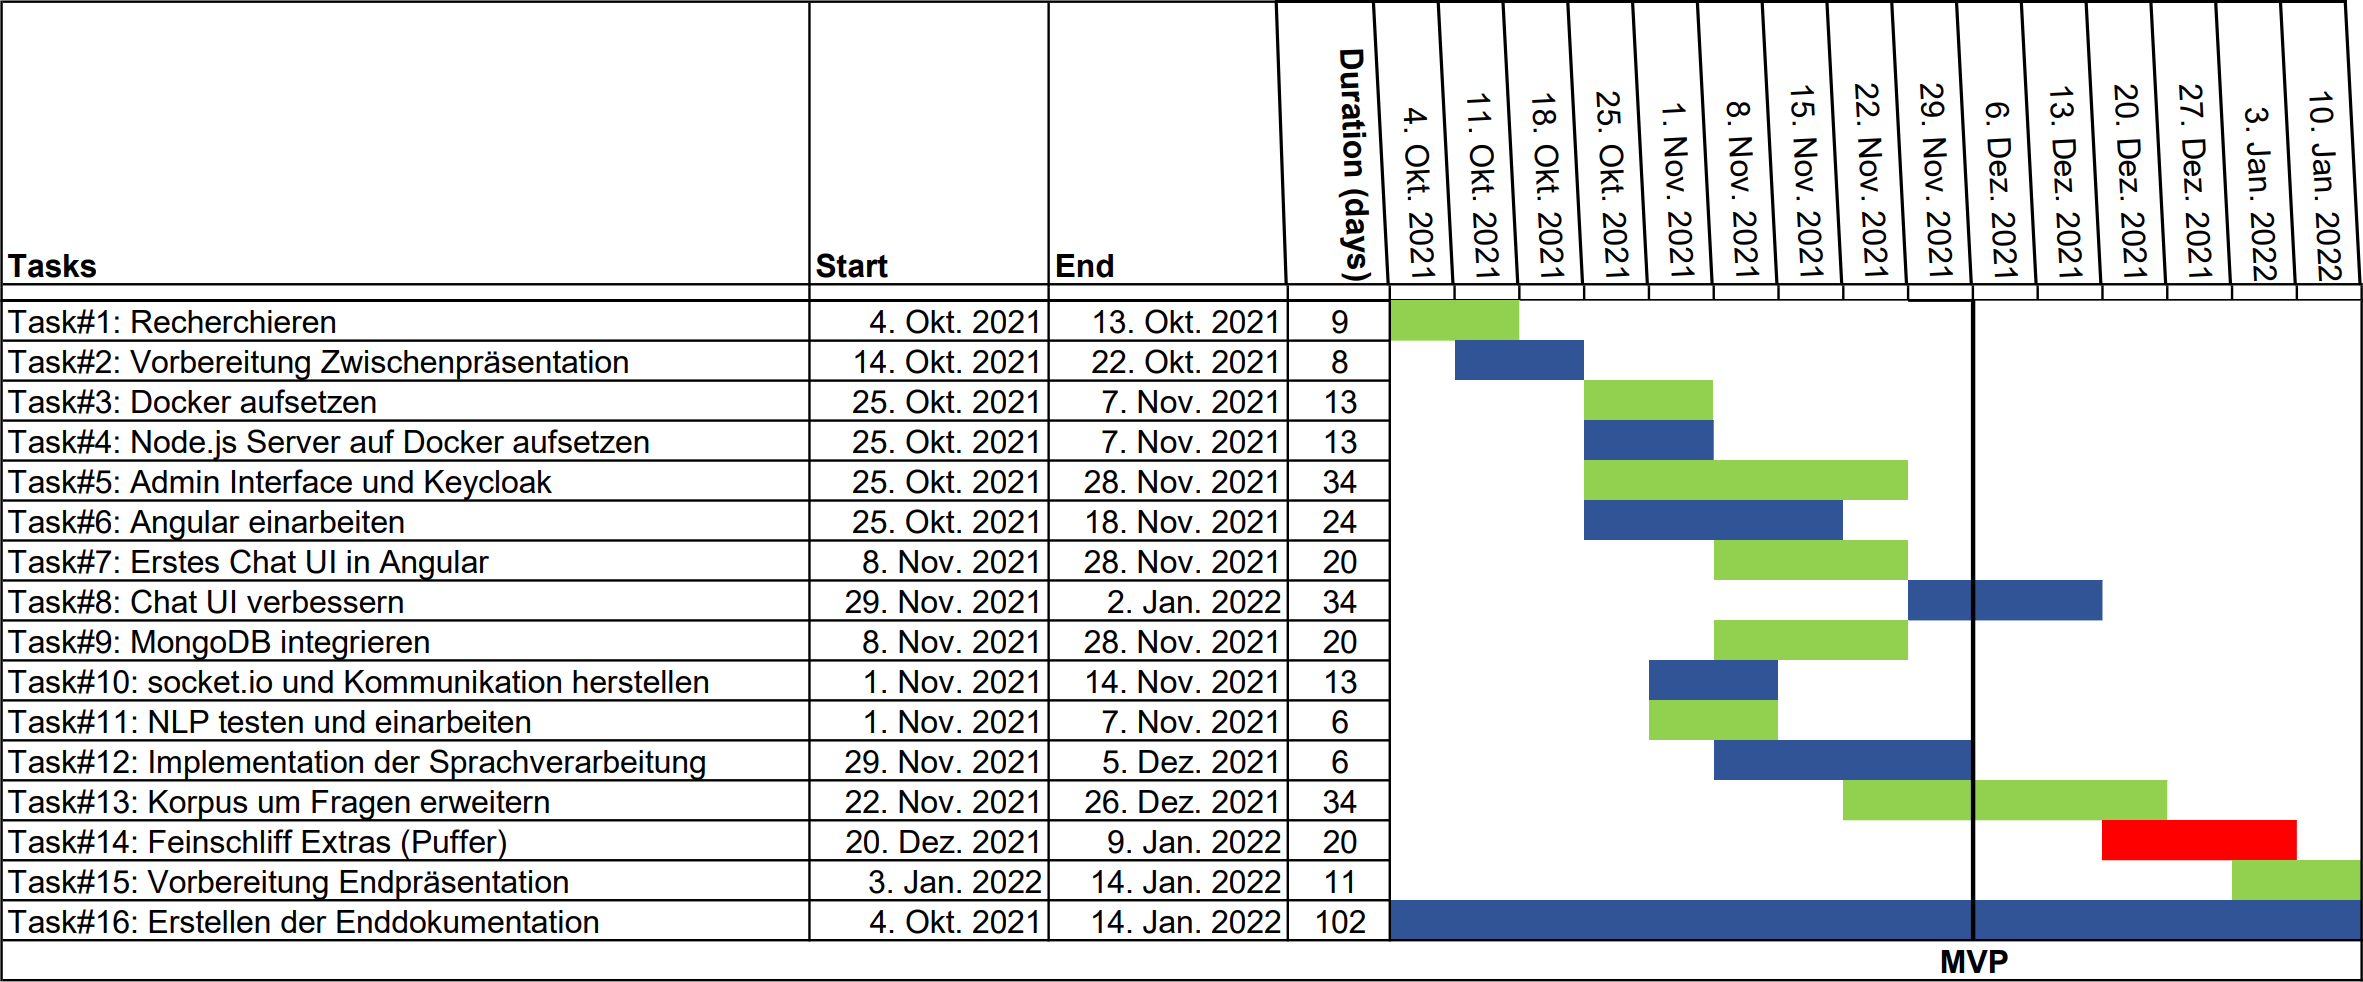
\includegraphics[width=1.0\textwidth]{bilder/zeitmanagement/gantt-diagramm.png}
\newpage
\section{Risikoanalyse}

Auf den folgenden Seiten haben wir in einer Tabelle möglicher Risiken für unser Projekt aufgelistet.
Sowie Maßnahmen wie wir diese Risiken verringern möchten. \\

\begin{table}[H]
    \begin{center}
        \begin{tabular}{|p{120px}|c|c|p{150px}|}
            \hline
            \begin{tabular}{l}
                Risiko \\
            \end{tabular}
             &
            \begin{tabular}{l}
                Eintritts-  \\
                wahrschein- \\
                lichkeit    \\
            \end{tabular}
             &
            \begin{tabular}{l}
                Auswirkung \\
            \end{tabular}
             &
            \begin{tabular}{l}
                Maßnahme \\
            \end{tabular}
            \\
            \hline
            \begin{tabular}{l}
                Team schafft es  \\
                nicht schnell    \\
                genug Typescript \\
                zu lernen        \\
            \end{tabular}
             &
            \begin{tabular}{l}
                niedrig \\
            \end{tabular}
             &
            \begin{tabular}{l}
                hoch \\
            \end{tabular}
             &
            \begin{tabular}{l}
                Alle Teammitglieder \\
                beginnen frühzeitig \\
                sich mit Typescript \\
                zu beschäftigen     \\
            \end{tabular}
            \\
            \hline
            \begin{tabular}{l}
                Team schafft es \\
                nicht Keycloak  \\
                zu integrieren  \\
            \end{tabular}
             &
            \begin{tabular}{l}
                niedrig \\
            \end{tabular}
             &
            \begin{tabular}{l}
                hoch \\
            \end{tabular}
             &
            \begin{tabular}{l}
                Alle Teammitglieder     \\
                schauen sich recht-     \\
                zeitig die Einführungs- \\
                videos von Herr Rößler  \\
                zu Keycloak an          \\
            \end{tabular}
            \\
            \hline
            \begin{tabular}{l}
                Das Team hat      \\
                Schwierigkeiten   \\
                das Userinterface \\
                in Angular zu     \\
                entwickeln        \\
            \end{tabular}
             &
            \begin{tabular}{l}
                niedrig \\
            \end{tabular}
             &
            \begin{tabular}{l}
                hoch \\
            \end{tabular}
             &
            \begin{tabular}{l}
                Das Team greift auf  \\
                gut bewährte Designs \\
                zurück               \\
            \end{tabular}
            \\
            \hline
            \begin{tabular}{l}
                Das Team hat    \\
                Schwierigkeiten \\
                eine Verbindung \\
                mit socket.io   \\
                herzustellen    \\
            \end{tabular}
             &
            \begin{tabular}{l}
                niedrig \\
            \end{tabular}
             &
            \begin{tabular}{l}
                hoch \\
            \end{tabular}
             &
            \begin{tabular}{l}
                Das Team informiert    \\
                sich rechtzeitig auf   \\
                der Socket.io Website, \\
                wie eine Verbindung    \\
                aufgebaut wird         \\
            \end{tabular}
            \\
            \hline
            \begin{tabular}{l}
                Das Admin Interface \\
                lässt sich nicht    \\
                flexibel genug      \\
                anpassen            \\
            \end{tabular}
             &
            \begin{tabular}{l}
                niedrig \\
            \end{tabular}
             &
            \begin{tabular}{l}
                niedrig \\
            \end{tabular}
             &
            \begin{tabular}{l}
                Das Team informiert     \\
                sich rechtzeitig        \\
                welche Möglichkeiten    \\
                es in das UI einbauen   \\
                möchte, um Flexibilität \\
                zu garantieren          \\
            \end{tabular}
            \\
            \hline
            \begin{tabular}{l}
                Der ChatBot     \\
                antwortet stark \\
                verzögert       \\
            \end{tabular}
             &
            \begin{tabular}{l}
                niedrig \\
            \end{tabular}
             &
            \begin{tabular}{l}
                mittel \\
            \end{tabular}
             &
            \begin{tabular}{l}
                Das Team muss mit-  \\
                einplanen, dass der \\
                ChatBot in kleine   \\
                saubere Module      \\
                aufgeteilt wird     \\
            \end{tabular}
            \\
            \hline
        \end{tabular}
    \end{center}
    \caption{Risikoanalyse Tabelle Teil 1}
    \label{tab:Risikoanalyse_Teil_1}
\end{table}
%Second part of the table
\begin{table}[H]
    \begin{center}
        \begin{tabular}{|p{120px}|c|c|p{150px}|}
                       \hline
            \begin{tabular}{l}
                Risiko \\
            \end{tabular}
             &
            \begin{tabular}{l}
                Eintritts-  \\
                wahrschein- \\
                lichkeit    \\
            \end{tabular}
             &
            \begin{tabular}{l}
                Auswirkung \\
            \end{tabular}
             &
            \begin{tabular}{l}
                Maßnahme \\
            \end{tabular}
            \\
            \hline
            \begin{tabular}{l}
                Hohe Latenz durch \\
                alle Komponenten  \\
            \end{tabular}
             &
            \begin{tabular}{l}
                unwahr-    \\
                scheinlich \\
            \end{tabular}
             &
            \begin{tabular}{l}
                mittel \\
            \end{tabular}
             &
            \begin{tabular}{l}
                Das Team muss den       \\
                ChatBot testen,         \\
                um z.B. Endlosschleifen \\
                zu verhindern           \\
            \end{tabular}
            \\
            \hline
            \begin{tabular}{l}
                Der ChatBot hat    \\
                Schwierigkeiten    \\
                Sätze zu verstehen \\
            \end{tabular}
             &
            \begin{tabular}{l}
                mittel \\
            \end{tabular}
             &
            \begin{tabular}{l}
                mittel \\
            \end{tabular}
             &
            \begin{tabular}{l}
                Das Team muss bei     \\
                einem Regex Ansatz    \\
                mehrere Regex Befehle \\
                vordefinieren, um ein \\
                großes Spektrum       \\
                abzudecken            \\
            \end{tabular}
            \\
            \hline
            \begin{tabular}{l}
                Die Hardware des \\
                Kunden ist nicht \\
                kompatibel mit   \\
                der Software     \\
            \end{tabular}
             &
            \begin{tabular}{l}
                niedrig \\
            \end{tabular}
             &
            \begin{tabular}{l}
                hoch \\
            \end{tabular}
             &
            \begin{tabular}{l}
                Das Team muss       \\
                frühzeitig mit dem  \\
                Kunden klären für   \\
                welche Hardware der \\
                ChatBot entwickelt  \\
                werden soll         \\
            \end{tabular}
            \\
            \hline
            \begin{tabular}{l}
                Das Team scheitert \\
                einen MVP zu       \\
                entwickeln         \\
            \end{tabular}
             &
            \begin{tabular}{l}
                niedrig \\
            \end{tabular}
             &
            \begin{tabular}{l}
                hoch \\
            \end{tabular}
             &
            \begin{tabular}{l}
                Das Team muss sehr    \\
                früh mit der Imple-   \\
                mentierung beginnen   \\
                und ausführlich genug \\
                recherchieren         \\
            \end{tabular}
            \\
            \hline
            \begin{tabular}{l}
                Das Team scheitert \\
                rechtzeitig genug  \\
                alle Technologien  \\
                zu lernen          \\
            \end{tabular}
             &
            \begin{tabular}{l}
                niedrig \\
            \end{tabular}
             &
            \begin{tabular}{l}
                hoch \\
            \end{tabular}
             &
            \begin{tabular}{l}
                Das Team recherchiert   \\
                frühzeitig und versucht \\
                für alle möglichen      \\
                Probleme Lösungen       \\
                zu finden               \\
            \end{tabular}
            \\
            \hline
        \end{tabular}
    \end{center}
    \caption{Risikoanalyse Tabelle Teil 2}
    \label{tab:Risikoanalyse_Teil_2}
\end{table}
\noindent Fazit: \\
Bei Beginn unseres Projektes haben wir mögliche Risiken aufgelistet,
die in unserem Projekt auftauchen könnten
und wie wir diese nach Möglichkeit verhindern möchten.
Wir haben dabei herausgefunden, dass wir sehr viele Risiken haben,
die von niedriger Eintrittswahrscheinlichkeit sind.
Dennoch sind die Mehrheit der Risiken von hoher Auswirkung im Projekt.
Als Beispiel, das Team schafft es nicht schnell genug Typescript zu lernen.
Die wichtigsten Risiken für uns waren die oben genannten Risiken zu Angular, Keycloak und Socket.io.
Wenn eines dieser Risiken von unserem Team nicht ausgleichbar wäre,
dann würden wir gar nicht die Möglichkeit haben einen MVP oder
später ein fertiges funktionierendes Produkt abzuliefern.
Mit den Tabellen \ref{tab:Risikoanalyse_Teil_1} und \ref{tab:Risikoanalyse_Teil_2}  möchten wir für unsere Gruppe festhalten,
welche Gedanken wir uns über die möglichen Risiken in unserem Projekt gemacht haben.
Damit wir besser und effizienter unser Projekt vorantreiben können und
vorbereitet sind auf mögliche Schwierigkeiten.
\newpage
\section{Aufteilung des Teams}
Hier werden die einzelnen Aufgaben, die wir bearbeitet haben in Issues mit dem Namen der Beteilligten aufgezählt.

\subsection{Herr Ralf Zeller}
Hier werden die Issues von Herr Ralf Zeller aufgelistet.
\begin{enumerate}
    \item Angular vs. React.js vs, Vue.js recherchiert
    \item Videoinhalt für die Zwischenpräsentation erstellt
    \item Die Zwischenpräsentationsfolien erstellt
    \item Latex Grundstruktur der Dokumentation erstellt
    \item Die Meilensteine in der Dokumentation erstellt
    \item Die Risk Liste erstellt
    \item Technologien in der Dokumentation eingetragen
    \item Die Commits und die Labeling bestimmen (in welcher Sprache und in welcher Form diese geschrieben werden)
    \item Die Datenbank für den Korpus erstellt
    \item Ausgetestet ob NLP mit mongoDB benutzt werden kann
    \item Datenbankstruktur (ERM) erstellt
    \item Die Technologien in der Dokumentation aktualisiert
    \item Den SRC von der "Literatur.bib" geprüft
    \item Risikoanalyse geprüft und ein Review geschrieben
    \item Meilensteine korrigiert
    \item Die Technologien geprüft und die Liste neu gestaltet
    \item Die Use Cases enummeriert
    \item Die Dokumentation Tree im Gitlab gesäubert
    \item Das UML Komponentendiagramm hinzugefügt
    \item Den NLP Node.js Server von  14+ zu 16+ aktualisiert
    \item Die Dokumentation korrigiert
    \item Die Admin development Branch gesäubert
    \item Docker Compose erstellt
    \item NLP Test Branch und presentation Branch rebased
    \item Chat/Admin UI, NLP und mongoDb kombiniert
    \item Admin Interface in Docker Compose integriert
    \item Funktionalität zu Admin Corpus Website hinzugefügt
    \item Keycloak in Docker Compose integriert
    \item Erste Version von der Dokumentation für die Abgabe hinzugefügt
    \item Versionen von allen Technologien überprüft
    \item NPM update am 11.01.22 durchgeführt
    \item Team Building Retrospective gehalten
    \item Corpus for Interna erstellt
    \item Die main Branch gesäubert
    \item Hinzufüge-/ und Entfern-/ Button für die Intent Cards im Admin Interface implementiert
    \item Die essentiellen Funktionen für die Rest API implementiert
    \item Allgemein und Einstellungen im Admin Interface bearbeitet
    \item Verbindung zwischen der Allgemein(General) Seite und dem Backend implementiert
    \item Verbindung zwischen Einstellungen(Settings) Seite und dem Backend implementiert
    \item JSON als Korpus in mongoDb integriert
    \item Den Hinzufüge Button auf der Korpus Seite ändern und den Entfernen Button integriert
    \item Installations- und Administrationshandbuch hinzugefügt
    \item Ausblick ausgedacht
    \item Fix Intent Cards in Container HTML intent-array Intent Karten in Container HTML intent-array fixiert
    \item Nicht benutzte Branches gelöscht
    \item Readme über Gitlab clean hinzugefügt
    \item Den Icon von der Katze im Chat Interface geändert
    \item READEME für questME Gitlab Repository hinzugefügt
    \item Die Technologien in der Dokumentation aktualisiert
    \item Alle Meeting Protokolle verfasst
    \item Alle Meeting Protokolle in die Dokumentation Branch gepusht
    \item UI in Englisch umgeschrieben
    \item Kapitel zu den Docker Images erstellt
\end{enumerate}

\subsection{Frau Pavithra Sureshkumar}
Hier werden die Issues von Frau Pavithra Sureshkumar aufgelistet.
\begin{enumerate}
    \item Am Anfang des Projekts: Aufgabenverteilung und Milestones mit Prioritäten erstellen
    \item Angular vs. React.js vs, Vue.js recherchiert
    \item Videoinhalt für die Zwischenpräsentation erstellt
    \item Die Zwischenpräsentationsfolien erstellt
    \item UI Designs erstellt und dokumentiert
    \item Use Cases erstellt und dokumentiert
    \item About Us hinzugefügt
    \item User Stories erstellt und dokumentiert
    \item Angular getestet und Chat Interface erstellt
    \item User stories neu formuliert
    \item getrennte Komponentendiagramme erstellt
    \item Kriterien für Usability erstellt
    \item Zielgruppe, Problem, Eigenschaften, Alleinstellungsmerkmal erstellt
    \item Merge fault von User Stories korrigiert
    \item Admin Interface mit Angular erstellt
    \item An Corpus gearbeitet
    \item Usability-Test erstellt und hinzugefügt
    \item UI Designs korrigiert
    \item Appendix erstellt
    \item Die Dokumentation Tree im Gitlab gesäubert
    \item User Story mit Acceptance Criteria erstellt und dokumentiert
    \item Den UML Komponentendiagramm hinzugefügt
    \item Die Admin development Branch gesäubert
    \item Funktionalität zu Admin Corpus Website hinzugefügt
    \item UI Designs Version 1/2 korrigiert
    \item Team Building Retrospective gehalten
    \item Corpus for University erstellt
    \item Corpus for Interna erstellt
    \item Angular CI/CD for automated testing recherchiert (aber keine Zeit gehabt auszutesten)
    \item Hinzufüge-/ und Entfern-/ Button für die Intent Cards im Admin Interface implementiert
    \item Allgemein und Einstellungen im Admin Interface gearbeitet
    \item Chat/Admin UI, NLP und mongoDb kombiniert
    \item Verbindung zwischen der Allgemein(General) Seite und Backend implementiert
    \item Verbindung zwischen Einstellungen(Settings) Seite und Backend implementiert
    \item Ein Hintergrundbild für den Chat hinzugefügt
    \item Auswahl an Hintergründen für den Chat erstellt
    \item Angefangen an der Enddokumentation zu arbeiten
    \item Installations- und Administrationshandbuch hinzugefügt
    \item Die Aufgabenverteilung von Ralf und Pavithra dokumentiert
    \item Die Reflektion vom Projektmanagement hinzugefügt
    \item Benutzte Lizenzen und Projekt Lizenzen eingetragen
    \item Ausblick ausgedacht und dokumentiert
    \item Team Reflektion vom Lernfortschritt verfasst und dokumentiert
    \item Angefangen die Endpräsentation vorzubereiten und Präsentationsfolien erstellt
    \item Endpräsentation korrigiert und bearbeitet
    \item Alle Meeting Protokolle verfasst
    \item Meeting Protokolle als PDF in Appendix (in Latex) hinzugefügt
    \item Aufgabenverteilung korrigiert
\end{enumerate}

\subsection{Herr Kevin Sautner}
Hier werden die Issues von Herr Kevin Sautner aufgelistet.
\begin{enumerate}
    \item Recherche zu MongoDB vs. PostgreSQL
    \item Tabellen MongoDB vs. PostgreSQL und Angular vs. Vue.js hinzugefügt
    \item Gantt-Diagramm überarbeitet und hinzugefügt
    \item UML-Verteilungsdiagramm erstellt und hinzugefügt
    \item Fazit zu den Technologien-Tabellen hinzugefügt
    \item Tests mit Keycloak durchgeführt
    \item Gantt-Diagramm um Milestones erweitert
    \item Zielgruppe Professor erstellt
    \item Beschreibung zum Gantt-Diagramm hinzugefügt
    \item Keycloak implementiert
    \item Gantt- und Verteilungsdiagramm überarbeitet
    \item Fazit zu Tabellen überarbeitet
    \item Teile der Use Cases und User Stories erstellen und überarbeitet
    \item Unterpunkte von Technologien neu angeordnet
    \item Rechtschreibprüfung der Dokumentation zur Zwischenabgabe
    \item Versucht Keycloak auf SAML umzustellen
    \item Grundstruktur der Rest-API erweitert
    \item Keycloak Authentifizierung in die Rest-API implementiert
    \item Auslesen und Senden der Nutzerrollen mit einer Chat-Nachricht
    \item Kapitel zur Sicherheit hinzugefügt
    \item UML-Verteilungsdiagramm angepasst
    \item Keycloak Administrationshandbuch hinzugefügt
\end{enumerate}
\newpage
\section{Reflektion Projektmanagement}
In diesem Abschnitt wird die Planung, die man vorgenommen hat
(in Meilensteine) reflektiert. 
Reflektiert wird, ob die Planung wie gehabt durchgeführt wurde und 
wie die Aufwandschätzung vom Geplanten und der Realisierung war.

\begin{table}[H]
    \begin{center}
        \begin{tabular}{|p{180px}|c|}
            \hline
            \begin{tabular}{l}
                \\
                \large Recherche \\
                \\
            \end{tabular}
             &
            \begin{tabular}{l}
                \\
                \large \bfseries 13.10.21 \\
                \\
            \end{tabular}
            \\
            \hline
            \begin{tabular}{l}
                \\
                \large Zwischenpräsentation \\
                \\
            \end{tabular}
             &
            \begin{tabular}{l}
                \\
                \large \bfseries 22.10.21 \\
                \\
            \end{tabular}
            \\
            \hline
            \begin{tabular}{l}
                \\
                \large Implementation \\
                \\
            \end{tabular}
             &
            \begin{tabular}{l}
                \\
                \large \bfseries 25.10.21 \\
                \\
            \end{tabular}
            \\
            \hline
            \begin{tabular}{l}
                \\
                \large MVP \\
                \\
            \end{tabular}
             &
            \begin{tabular}{l}
                \\
                \large \bfseries  02.12.21 \\
                \\
            \end{tabular}
            \\
            \hline
            \begin{tabular}{l}
                \\
                \large \bfseries Endpräsentation und \\
                \large \bfseries Enddokumentation\\
                \\
            \end{tabular}
             &
            \begin{tabular}{l}
                \large \bfseries 14.01.22 \\
            \end{tabular}
            \\
            \hline
        \end{tabular}
        \caption{Meilenstein Liste}
        \label{tab:Meilenstein Liste}
    \end{center}
\end{table}

\subsection{Geplante Meilensteine für Reflektion}
Hier werden die Meilensteine, die man als Ziel gesetzt hat verglichen 
mit dem realen Aufwand.

\subsubsection{Recherche 13.10.21}
Die Recherche lief nach Plan. Was aber nicht ging, alles bis 13.10.21 zu lernen, 
da wir sehr viel zu Erfüllen hatten und nur drei Personen waren, mussten wir kontinuierlich Lernen. 
So musste nicht nur ein Bereich gelernt werden, sondern wir mussten uns Austauschen und unsere Codes vergleichen und zusammenfügen. 
Dies hat uns dann noch mehr Zeit gekostet als erwartet und wir sind auf kontinuierliche Recherche umgestiegen.

\subsubsection{Zwischenpräsentation 22.10.21}
Bei der Zwischenpräsentation haben wir uns sehr viel Zeit genommen uns eine kreative Idee auszudenken, 
was uns von den anderen Gruppen unterscheidet und wie wir unsere Präsentation so einfach wie möglich darstellen. 
Die Zwischenpräsentation mussten wir auch sehr schnell erledigen und hatten kaum Zeit zu üben, da diese nach einem kurzen Zeitraum stattfand. 
Wir haben uns aber trotzdem in der Hochschule getroffen und haben im Präsentationsraum unsere Präsentation Test geprobt, 
um uns vorzubereiten und unsere Ressourcen auszutesten, wie Ton, Laptop verbinden und das Reden mit der Mundschutzmaske nicht zu vergessen.

\subsubsection{Implementation 25.10.21}
Die Implementation dauert noch bis 11.01.22 an und ist gerade dabei noch ein Feinschlief durchzulaufen. 
Das wichtigste für uns ist hierbei das Produkt so weit wie möglich präsentabel zu programmieren. 
Die Implementation lief sehr schwergängig, da wir auch sehr viel zu tun hatten mit nur drei Gruppenmitglieder. 
Hinzu kam es noch, dass sich Probleme beim Implementieren ergeben haben, aber diese von uns wieder durch Pair Programming gelöst wurde. 

\subsubsection{MVP und Codereview 02.12.21}
Das MVP oder auch technischer Durchstich genannt haben wir sehr gut hinbekommen. 
Das wichtigste hierbei war das Codereview. Beim Codereview mussten wir unsere Codes vorstellen, damit wir auch zeigen können wer welche Aufgaben gelöst hat. 
Wir wollten unser MVP mehr ausreifen, aber hatten wieder das zeitliche Problem, Probleme Wissenslücken zu füllen und das Problem Codes zu kombinieren damit diese auch funktionieren. 

\subsubsection{Endpräsentation und Enddokumentation 14.01.22}
Bei der Endpräsentation haben wir uns vorgenommen früher vorzunehmen, aber wir konnten es aus zeitlichen Gründen nicht eine Woche früher vorbereiten.
Wir müssen nämlich auch den ChatBot ausbessern und einen Feinschliff durchführen. Die Präsentation kann nur vorbereitet werden, wenn der ChatBot fertig und vorführbar ist. 
Diese haben wir geplant am 11.01.22 fertig zu haben, damit wir noch bis zu der Präsentation üben können,
um die Präsentation so gut wie möglich vorzuführen
Die Enddokumentation wird schon von Anfang an verfasst und wird dann mit der Endpräsentation abgegeben.
\newpage
\section{Reflektion Lernfortschritt}
Hier wird der Lernforschritt, den wir als Gruppe gesammelt haben beschrieben.

\subsection{Reflektion Lernfortschritt als Team}
In unserem Projekt haben wir sehr viel Neues gelernt. Wir haben nicht nur fachliches Wissen erweitert und eingesetzt, sondern auch Teambildung und Teamarbeit ausgeführt. Wir haben trotz dass wir nur drei Personen sind, versucht Scrum auszuführen.\newline
Das ein Team nicht immer einwandfrei läuft ist selbstverständlich. 
Es können immer Probleme bei Kommunikation entstehen und man könnte etwas falsch verstehen oder übermitteln. 
Dafür haben wir eine Retrospektive gemacht. Wir haben unsere Probleme angesprochen und eine Lösung gefunden. 
Auch haben wir gelernt, dass manche nicht die Motivation gehabt haben etwas im Team zu leisten. Wir haben beschlossen dann etwas als Team zu unternehmen, um den Teamgeist zu steigern. 
Mit unserem Betreuer haben wir immer versucht jede Woche eine Besprechung zu halten und haben diese auch immer dokumentiert und immer nach der Besprechung zusammengefasst und es dem Meeting Mitglieder geschickt, um den Überblick zu behalten. 
Auch wenn man sich austauscht, sollte aber in jedem Team das selbstständige Arbeiten nicht ausfallen. Mit dem selbstständigen Arbeiten ist gemeint, 
dass man Aufgaben übernimmt und nicht zugeteilt bekommt, das heißt Eigeninitiative sollte bei jedem vorhanden sein. Diese erwies sich schwer, weil es immer verschiedene Arbeitscharaktere gibt. 
Manche können nicht sich organisieren oder Selbstständigkeit vermitteln oder müssen extra Motivation finden. Das alles haben wir im Seminar gelernt und ist für uns eine große Lehre.\newline
Außerdem haben wir die Planung unterschätzt. Wir hätten strenge Regeln setzen müssen, damit die Aufgabenverteilung gerecht verteilt wird. 
Dadurch, dass man es nicht gemacht hat, haben einige in der Gruppe mehr machen müssen und haben auf Hilfe des anderen gewartet, die nie ankam. Am Anfang wurde die Planung so ausgeführt, dass sich jeder mit seinem Thema beschäftigt und schon was macht. 
Leider wurde diese Aufgabe nicht ernst genommen und es kam dazu, dass sich ein paar Gruppenmitglieder mit sehr viel Arbeit überbelastet haben. Am Ende haben wir noch versucht die Aufgabenverteilung gerechter zu machen. 

\newpage
\section{Ausblick: Pläne für die Zukunft}
Hier werden die möglichen Ergänzungen in unserem Projekt erwähnt.

\subsection{Mögliche Ergänzungen in der Zukunft}
Hier werden die Ergänzungen aufgelistet.

\begin{itemize}
    \item CSV importieren von Intents
    \item Mehr individuelles Gestalten der Chat Seite
    \item Mehr Korpusdaten 
    \item Mehr Domänen und Gruppen
    \item Nicht nur lokaler Zugang
    \item questMe in mehreren Plattformen integrieren
    \item Paginator für Korpusdaten
\end{itemize}
\newpage
\section{Appendix}
Hier werden die extra Content abgebildet.

\subsection{Ältere Versionen des Komponentendiagramms}

\subsubsection{Komponentendiagramme}

\begin{figure}[H]
\centering
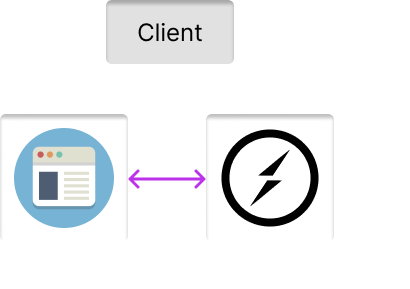
\includegraphics[width=0.5\textwidth]{bilder/technologien/KomponentendiagramClient.png}
\caption{Komponentendiagramm Client}
\label{fig:Komponentendiagramm_Client}
\end{figure}
Hier wird die Client Seite bildlich dargestellt. Man sieht, dass der Webbrowseer durch die 
Socket.io Client deployed wird und dadurch wird dann eine Beziehung zur Serverseite aufgebaut. (Siehe Abbildung \ref{fig:Komponentendiagramm_Client})

\begin{figure}[H]
\centering
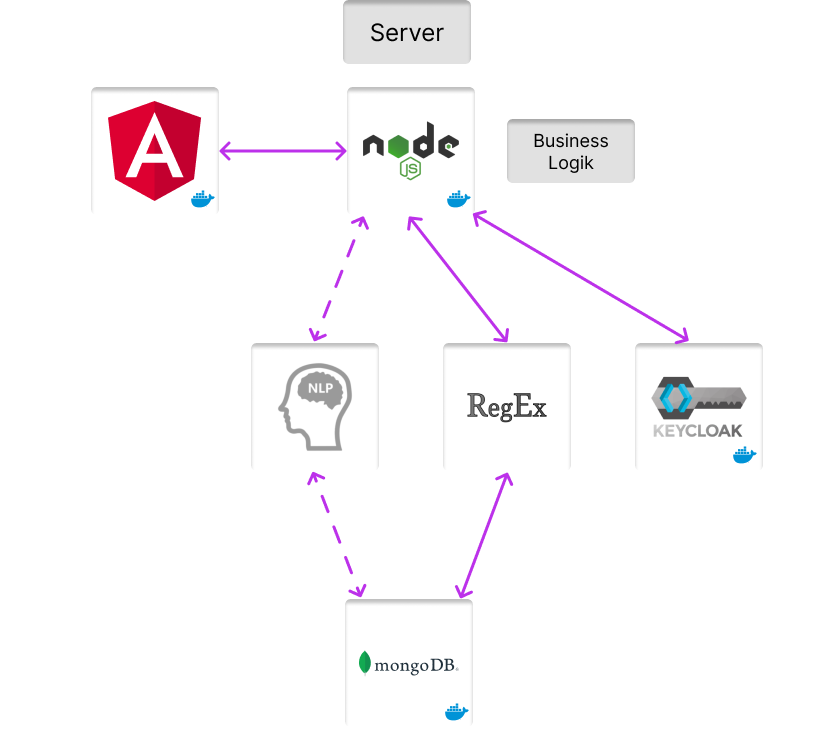
\includegraphics[width=0.9\textwidth]{bilder/technologien/KomponentendiagramServer.png}
\caption{Komponentendiagramm Server}
\label{fig:Komponentendiagramm_Server}
\end{figure}

\noindent In der Serverseite wird dann durch den Socket.io Server die Verbindug zum Clienten aufrecht gehalten.
Im Server befindet sich Angular, node.js, KeyCloak und die Datenbank mongoDB und haben jeweils einen eigenen Dockercontainer. 
Die Erkennung von der eingegeben Sprache möchten wir zunächst mit RegEx ermöglichen, 
um das Minimal Viable Product hinzubekommen. Optional dann mit NLP (Natural Language Processing) erweitern.

\begin{figure}[!hbt]
    \centering
    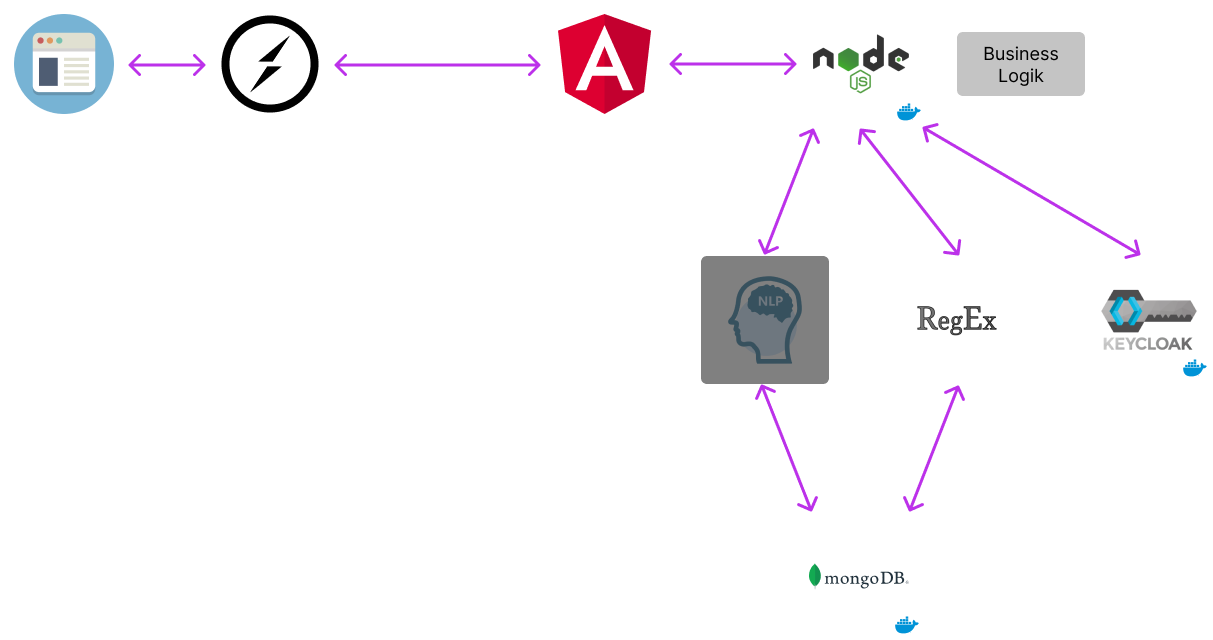
\includegraphics[width=1.0\textwidth]{bilder/technologien/Komponenten-Diagram-v1.png}
    \caption{Komponentendiagramm v1.0}
    \label{fig:Komponentendiagramm_v1.0}
    \end{figure}

\noindent In dieser Version haben wir erst einmal die Struktur von unseren Komponentengesucht und eine
grobe Darstellung erstellt. Was wir hier aber nicht wussten ist, wie wir das NLP darstellen sollten.
NLP war für uns vorher eine optionale Möglichkeit.

    \begin{figure}[!hbt]
        \centering
        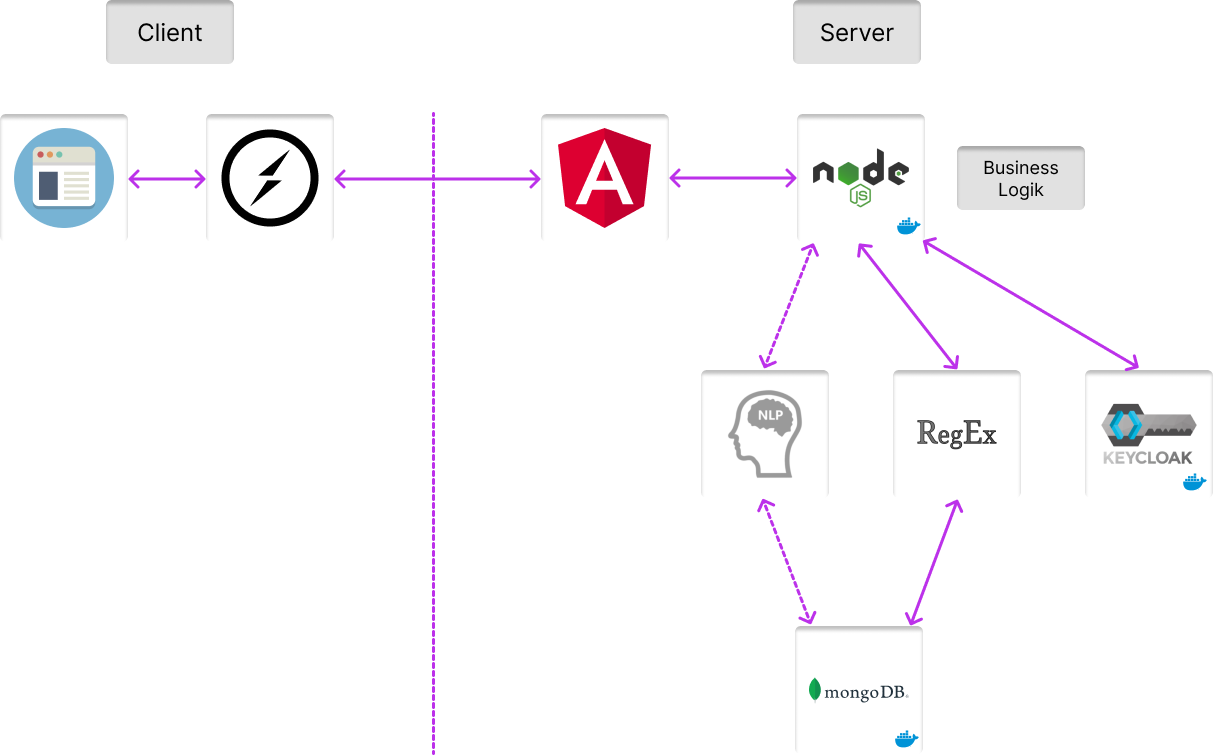
\includegraphics[width=1.0\textwidth]{bilder/technologien/Komponentendiagram v1.1.png}
        \caption{Komponentendiagramm v1.1}
        \label{fig:Komponentendiagramm_v1.1}
        \end{figure}
        \FloatBarrier 

\noindent In dieser Darstellung haben wir die einzelnen Komponenten in Server und Client 
eingeteilt, um die Struktur besser zu verstehen. Wir haben aber die Abtrennung nicht richtig anzeigen können
und das NLP haben wir auch nicht klar als optional zeigen können.

    \begin{figure}[!hbt]
        \centering
        \includegraphics[width=1.0\textwidth]{bilder/technologien/Komponentendiagram v1.2.png}
        \caption{Komponentendiagramm v1.2}
        \label{fig:Komponentendiagramm_v1.2}
        \end{figure}
        \FloatBarrier % prevent pictures from appearing under a different section
    
\section{Meeting Protokolle}
Hier werden die Meeting Protokolle von unseren Besprechungen mit Herr Watzko, Herr Renz und Herr Rößler protokolliert.

\subsection{Protokolle in PDFs eingebunden}
Hier werden die Protokolle als PDFs eingebunden. Diese werden von alt bis neu aufgelistet.

\includepdf[pages=-]{protocols/Protokoll_08_10_21_Team questMe.pdf}
\includepdf[pages=-]{protocols/Protokoll_13_10_21_Team_questMe.pdf}
\includepdf[pages=-]{protocols/Protokoll_19_10_21_Team_questMe.pdf}
\includepdf[pages=-]{protocols/Protokoll_20_10_21_Team_questMe.pdf}
\includepdf[pages=-]{protocols/Protokoll_29_10_21_Team_questMe.pdf}
\includepdf[pages=-]{protocols/Protokoll_12_11_21_Team_questMe.pdf}
\includepdf[pages=-]{protocols/Protokoll_19_11_21_Team_questMe.pdf}
\includepdf[pages=-]{protocols/Protokoll_26_11_21_Team_questMe.pdf}
\includepdf[pages=-]{protocols/Protokoll_03_12_21_Team_questMe.pdf}
\includepdf[pages=-]{protocols/Protokoll_10_12_21_Team_questMe.pdf}
\includepdf[pages=-]{protocols/Protokoll_17_12_21_Team_questMe.pdf}
\includepdf[pages=-]{protocols/Protokoll_22_12_21_Team_questMe.pdf}
\includepdf[pages=-]{protocols/Protokoll_12_01_22_Team_questMe.pdf}
\newpage
% Sources
\addcontentsline{toc}{section}{Literatur}
\printbibliography

\end{document}
